\section{Controller Performance}
\label{sec:results:performance}

\begin{figure}
  \centering
  \begin{subfigure}{0.48\linewidth}
    \footnotesize
    % This file was created by matlab2tikz.
%
\definecolor{mycolor1}{rgb}{0.00000,0.44700,0.74100}%
\definecolor{mycolor2}{rgb}{0.85000,0.32500,0.09800}%
\definecolor{mycolor3}{rgb}{0.92900,0.69400,0.12500}%
%
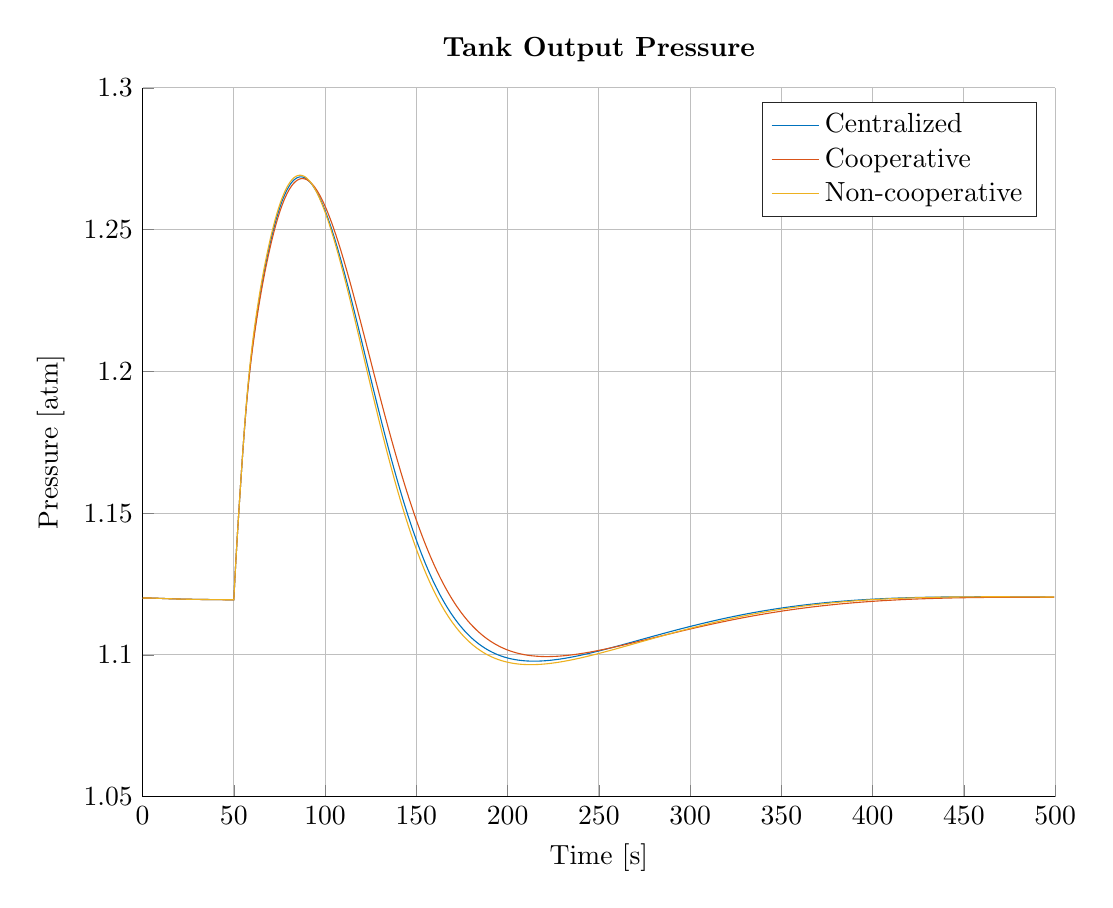
\begin{tikzpicture}

\begin{axis}[%
width=4.563in,
height=3.544in,
at={(0.792in,0.541in)},
scale only axis,
xmin=0,
xmax=500,
xlabel={Time [s]},
xmajorgrids,
ymin=1.05,
ymax=1.3,
ylabel={Pressure [atm]},
ymajorgrids,
axis background/.style={fill=white},
title style={font=\bfseries},
title={Tank Output Pressure},
axis x line*=bottom,
axis y line*=left,
legend style={legend cell align=left,align=left,draw=white!15!black}
]
\addplot [color=mycolor1,solid,forget plot]
  table[row sep=crcr]{%
0	1.12\\
0.5	1.12007\\
1	1.12008\\
1.5	1.12008\\
2	1.12008\\
2.5	1.12008\\
3	1.12008\\
3.5	1.12007\\
4	1.12007\\
4.5	1.12006\\
5	1.12005\\
5.5	1.12004\\
6	1.12003\\
6.5	1.12002\\
7	1.12001\\
7.5	1.12\\
8	1.11999\\
8.5	1.11997\\
9	1.11996\\
9.5	1.11995\\
10	1.11994\\
10.5	1.11992\\
11	1.11991\\
11.5	1.1199\\
12	1.11989\\
12.5	1.11987\\
13	1.11986\\
13.5	1.11985\\
14	1.11984\\
14.5	1.11983\\
15	1.11981\\
15.5	1.1198\\
16	1.11979\\
16.5	1.11978\\
17	1.11977\\
17.5	1.11976\\
18	1.11975\\
18.5	1.11974\\
19	1.11973\\
19.5	1.11973\\
20	1.11972\\
20.5	1.11971\\
21	1.1197\\
21.5	1.11969\\
22	1.11969\\
22.5	1.11968\\
23	1.11967\\
23.5	1.11966\\
24	1.11966\\
24.5	1.11965\\
25	1.11964\\
25.5	1.11964\\
26	1.11963\\
26.5	1.11962\\
27	1.11962\\
27.5	1.11961\\
28	1.11961\\
28.5	1.1196\\
29	1.1196\\
29.5	1.11959\\
30	1.11959\\
30.5	1.11958\\
31	1.11958\\
31.5	1.11957\\
32	1.11957\\
32.5	1.11956\\
33	1.11956\\
33.5	1.11955\\
34	1.11955\\
34.5	1.11954\\
35	1.11954\\
35.5	1.11954\\
36	1.11953\\
36.5	1.11953\\
37	1.11952\\
37.5	1.11952\\
38	1.11952\\
38.5	1.11951\\
39	1.11951\\
39.5	1.11951\\
40	1.1195\\
40.5	1.1195\\
41	1.1195\\
41.5	1.11949\\
42	1.11949\\
42.5	1.11949\\
43	1.11949\\
43.5	1.11948\\
44	1.11948\\
44.5	1.11948\\
45	1.11948\\
45.5	1.11947\\
46	1.11947\\
46.5	1.11947\\
47	1.11947\\
47.5	1.11946\\
48	1.11946\\
48.5	1.11946\\
49	1.11946\\
49.5	1.11946\\
50	1.11945\\
50.5	1.12569\\
51	1.13171\\
51.5	1.13735\\
52	1.14274\\
52.5	1.14794\\
53	1.153\\
53.5	1.15795\\
54	1.1628\\
54.5	1.16756\\
55	1.17229\\
55.5	1.17676\\
56	1.18105\\
56.5	1.18514\\
57	1.189\\
57.5	1.1926\\
58	1.19596\\
58.5	1.19912\\
59	1.2021\\
59.5	1.20491\\
60	1.20757\\
60.5	1.21011\\
61	1.21253\\
61.5	1.21486\\
62	1.21711\\
62.5	1.21928\\
63	1.22138\\
63.5	1.22342\\
64	1.22541\\
64.5	1.22733\\
65	1.22921\\
65.5	1.23103\\
66	1.2328\\
66.5	1.23452\\
67	1.2362\\
67.5	1.23784\\
68	1.23943\\
68.5	1.24099\\
69	1.2425\\
69.5	1.24397\\
70	1.2454\\
70.5	1.24679\\
71	1.24814\\
71.5	1.24944\\
72	1.2507\\
72.5	1.25192\\
73	1.2531\\
73.5	1.25424\\
74	1.25533\\
74.5	1.25637\\
75	1.25738\\
75.5	1.25834\\
76	1.25925\\
76.5	1.26012\\
77	1.26095\\
77.5	1.26174\\
78	1.26248\\
78.5	1.26317\\
79	1.26383\\
79.5	1.26444\\
80	1.26501\\
80.5	1.26553\\
81	1.26602\\
81.5	1.26646\\
82	1.26686\\
82.5	1.26721\\
83	1.26753\\
83.5	1.2678\\
84	1.26804\\
84.5	1.26823\\
85	1.26839\\
85.5	1.2685\\
86	1.26858\\
86.5	1.26861\\
87	1.26861\\
87.5	1.26857\\
88	1.26849\\
88.5	1.26838\\
89	1.26823\\
89.5	1.26804\\
90	1.26782\\
90.5	1.26756\\
91	1.26727\\
91.5	1.26695\\
92	1.26659\\
92.5	1.2662\\
93	1.26577\\
93.5	1.26532\\
94	1.26483\\
94.5	1.26431\\
95	1.26376\\
95.5	1.26318\\
96	1.26258\\
96.5	1.26194\\
97	1.26128\\
97.5	1.26059\\
98	1.25987\\
98.5	1.25913\\
99	1.25836\\
99.5	1.25757\\
100	1.25675\\
100.5	1.25591\\
101	1.25504\\
101.5	1.25415\\
102	1.25324\\
102.5	1.25231\\
103	1.25136\\
103.5	1.25039\\
104	1.2494\\
104.5	1.24839\\
105	1.24736\\
105.5	1.24631\\
106	1.24525\\
106.5	1.24417\\
107	1.24307\\
107.5	1.24196\\
108	1.24083\\
108.5	1.23969\\
109	1.23854\\
109.5	1.23737\\
110	1.23619\\
110.5	1.235\\
111	1.2338\\
111.5	1.23258\\
112	1.23136\\
112.5	1.23012\\
113	1.22888\\
113.5	1.22763\\
114	1.22637\\
114.5	1.2251\\
115	1.22382\\
115.5	1.22254\\
116	1.22126\\
116.5	1.21996\\
117	1.21866\\
117.5	1.21736\\
118	1.21606\\
118.5	1.21474\\
119	1.21343\\
119.5	1.21212\\
120	1.2108\\
120.5	1.20948\\
121	1.20816\\
121.5	1.20683\\
122	1.20551\\
122.5	1.20419\\
123	1.20287\\
123.5	1.20155\\
124	1.20023\\
124.5	1.19891\\
125	1.19759\\
125.5	1.19628\\
126	1.19497\\
126.5	1.19366\\
127	1.19235\\
127.5	1.19105\\
128	1.18976\\
128.5	1.18847\\
129	1.18718\\
129.5	1.1859\\
130	1.18462\\
130.5	1.18335\\
131	1.18208\\
131.5	1.18082\\
132	1.17957\\
132.5	1.17833\\
133	1.17709\\
133.5	1.17586\\
134	1.17464\\
134.5	1.17342\\
135	1.17221\\
135.5	1.17101\\
136	1.16982\\
136.5	1.16864\\
137	1.16747\\
137.5	1.1663\\
138	1.16515\\
138.5	1.164\\
139	1.16287\\
139.5	1.16174\\
140	1.16062\\
140.5	1.15952\\
141	1.15842\\
141.5	1.15734\\
142	1.15626\\
142.5	1.1552\\
143	1.15414\\
143.5	1.1531\\
144	1.15207\\
144.5	1.15104\\
145	1.15003\\
145.5	1.14903\\
146	1.14804\\
146.5	1.14707\\
147	1.1461\\
147.5	1.14514\\
148	1.1442\\
148.5	1.14327\\
149	1.14235\\
149.5	1.14144\\
150	1.14054\\
150.5	1.13965\\
151	1.13878\\
151.5	1.13792\\
152	1.13706\\
152.5	1.13622\\
153	1.13539\\
153.5	1.13458\\
154	1.13377\\
154.5	1.13297\\
155	1.13219\\
155.5	1.13142\\
156	1.13066\\
156.5	1.12991\\
157	1.12917\\
157.5	1.12844\\
158	1.12773\\
158.5	1.12702\\
159	1.12633\\
159.5	1.12565\\
160	1.12498\\
160.5	1.12432\\
161	1.12367\\
161.5	1.12303\\
162	1.1224\\
162.5	1.12178\\
163	1.12117\\
163.5	1.12058\\
164	1.11999\\
164.5	1.11941\\
165	1.11885\\
165.5	1.11829\\
166	1.11775\\
166.5	1.11721\\
167	1.11669\\
167.5	1.11617\\
168	1.11566\\
168.5	1.11517\\
169	1.11468\\
169.5	1.1142\\
170	1.11373\\
170.5	1.11327\\
171	1.11282\\
171.5	1.11238\\
172	1.11195\\
172.5	1.11153\\
173	1.11111\\
173.5	1.11071\\
174	1.11031\\
174.5	1.10992\\
175	1.10954\\
175.5	1.10917\\
176	1.1088\\
176.5	1.10844\\
177	1.1081\\
177.5	1.10775\\
178	1.10742\\
178.5	1.1071\\
179	1.10678\\
179.5	1.10647\\
180	1.10616\\
180.5	1.10587\\
181	1.10558\\
181.5	1.1053\\
182	1.10502\\
182.5	1.10475\\
183	1.10449\\
183.5	1.10423\\
184	1.10399\\
184.5	1.10374\\
185	1.10351\\
185.5	1.10328\\
186	1.10305\\
186.5	1.10284\\
187	1.10262\\
187.5	1.10242\\
188	1.10222\\
188.5	1.10202\\
189	1.10184\\
189.5	1.10165\\
190	1.10147\\
190.5	1.1013\\
191	1.10113\\
191.5	1.10097\\
192	1.10081\\
192.5	1.10066\\
193	1.10051\\
193.5	1.10037\\
194	1.10023\\
194.5	1.1001\\
195	1.09997\\
195.5	1.09985\\
196	1.09973\\
196.5	1.09961\\
197	1.0995\\
197.5	1.09939\\
198	1.09929\\
198.5	1.09919\\
199	1.0991\\
199.5	1.09901\\
200	1.09892\\
200.5	1.09884\\
201	1.09876\\
201.5	1.09868\\
202	1.09861\\
202.5	1.09854\\
203	1.09848\\
203.5	1.09841\\
204	1.09836\\
204.5	1.0983\\
205	1.09825\\
205.5	1.0982\\
206	1.09815\\
206.5	1.09811\\
207	1.09807\\
207.5	1.09803\\
208	1.098\\
208.5	1.09797\\
209	1.09794\\
209.5	1.09791\\
210	1.09789\\
210.5	1.09787\\
211	1.09785\\
211.5	1.09784\\
212	1.09782\\
212.5	1.09781\\
213	1.09781\\
213.5	1.0978\\
214	1.0978\\
214.5	1.0978\\
215	1.0978\\
215.5	1.0978\\
216	1.0978\\
216.5	1.09781\\
217	1.09782\\
217.5	1.09783\\
218	1.09785\\
218.5	1.09786\\
219	1.09788\\
219.5	1.0979\\
220	1.09792\\
220.5	1.09794\\
221	1.09796\\
221.5	1.09799\\
222	1.09802\\
222.5	1.09805\\
223	1.09808\\
223.5	1.09811\\
224	1.09814\\
224.5	1.09818\\
225	1.09822\\
225.5	1.09826\\
226	1.0983\\
226.5	1.09834\\
227	1.09838\\
227.5	1.09842\\
228	1.09847\\
228.5	1.09851\\
229	1.09856\\
229.5	1.09861\\
230	1.09866\\
230.5	1.09871\\
231	1.09876\\
231.5	1.09882\\
232	1.09887\\
232.5	1.09893\\
233	1.09899\\
233.5	1.09904\\
234	1.0991\\
234.5	1.09916\\
235	1.09922\\
235.5	1.09928\\
236	1.09935\\
236.5	1.09941\\
237	1.09947\\
237.5	1.09954\\
238	1.0996\\
238.5	1.09967\\
239	1.09974\\
239.5	1.09981\\
240	1.09988\\
240.5	1.09995\\
241	1.10002\\
241.5	1.10009\\
242	1.10016\\
242.5	1.10023\\
243	1.10031\\
243.5	1.10038\\
244	1.10045\\
244.5	1.10053\\
245	1.1006\\
245.5	1.10068\\
246	1.10076\\
246.5	1.10083\\
247	1.10091\\
247.5	1.10099\\
248	1.10107\\
248.5	1.10115\\
249	1.10123\\
249.5	1.10131\\
250	1.10139\\
};
\addplot [color=mycolor1,solid]
  table[row sep=crcr]{%
250	1.10139\\
250.5	1.10147\\
251	1.10155\\
251.5	1.10163\\
252	1.10172\\
252.5	1.1018\\
253	1.10188\\
253.5	1.10196\\
254	1.10205\\
254.5	1.10213\\
255	1.10222\\
255.5	1.1023\\
256	1.10239\\
256.5	1.10247\\
257	1.10256\\
257.5	1.10264\\
258	1.10273\\
258.5	1.10281\\
259	1.1029\\
259.5	1.10299\\
260	1.10307\\
260.5	1.10316\\
261	1.10325\\
261.5	1.10334\\
262	1.10342\\
262.5	1.10351\\
263	1.1036\\
263.5	1.10369\\
264	1.10378\\
264.5	1.10386\\
265	1.10395\\
265.5	1.10404\\
266	1.10413\\
266.5	1.10422\\
267	1.10431\\
267.5	1.1044\\
268	1.10448\\
268.5	1.10457\\
269	1.10466\\
269.5	1.10475\\
270	1.10484\\
270.5	1.10493\\
271	1.10502\\
271.5	1.10511\\
272	1.1052\\
272.5	1.10529\\
273	1.10538\\
273.5	1.10546\\
274	1.10555\\
274.5	1.10564\\
275	1.10573\\
275.5	1.10582\\
276	1.10591\\
276.5	1.106\\
277	1.10609\\
277.5	1.10618\\
278	1.10627\\
278.5	1.10635\\
279	1.10644\\
279.5	1.10653\\
280	1.10662\\
280.5	1.10671\\
281	1.1068\\
281.5	1.10688\\
282	1.10697\\
282.5	1.10706\\
283	1.10715\\
283.5	1.10724\\
284	1.10732\\
284.5	1.10741\\
285	1.1075\\
285.5	1.10759\\
286	1.10767\\
286.5	1.10776\\
287	1.10785\\
287.5	1.10793\\
288	1.10802\\
288.5	1.1081\\
289	1.10819\\
289.5	1.10828\\
290	1.10836\\
290.5	1.10845\\
291	1.10853\\
291.5	1.10862\\
292	1.1087\\
292.5	1.10879\\
293	1.10887\\
293.5	1.10896\\
294	1.10904\\
294.5	1.10912\\
295	1.10921\\
295.5	1.10929\\
296	1.10937\\
296.5	1.10946\\
297	1.10954\\
297.5	1.10962\\
298	1.1097\\
298.5	1.10979\\
299	1.10987\\
299.5	1.10995\\
300	1.11003\\
300.5	1.11011\\
301	1.11019\\
301.5	1.11027\\
302	1.11035\\
302.5	1.11043\\
303	1.11051\\
303.5	1.11059\\
304	1.11067\\
304.5	1.11075\\
305	1.11083\\
305.5	1.1109\\
306	1.11098\\
306.5	1.11106\\
307	1.11114\\
307.5	1.11121\\
308	1.11129\\
308.5	1.11137\\
309	1.11144\\
309.5	1.11152\\
310	1.11159\\
310.5	1.11167\\
311	1.11174\\
311.5	1.11182\\
312	1.11189\\
312.5	1.11197\\
313	1.11204\\
313.5	1.11211\\
314	1.11219\\
314.5	1.11226\\
315	1.11233\\
315.5	1.1124\\
316	1.11248\\
316.5	1.11255\\
317	1.11262\\
317.5	1.11269\\
318	1.11276\\
318.5	1.11283\\
319	1.1129\\
319.5	1.11297\\
320	1.11304\\
320.5	1.11311\\
321	1.11317\\
321.5	1.11324\\
322	1.11331\\
322.5	1.11338\\
323	1.11344\\
323.5	1.11351\\
324	1.11358\\
324.5	1.11364\\
325	1.11371\\
325.5	1.11377\\
326	1.11384\\
326.5	1.1139\\
327	1.11397\\
327.5	1.11403\\
328	1.11409\\
328.5	1.11416\\
329	1.11422\\
329.5	1.11428\\
330	1.11434\\
330.5	1.11441\\
331	1.11447\\
331.5	1.11453\\
332	1.11459\\
332.5	1.11465\\
333	1.11471\\
333.5	1.11477\\
334	1.11483\\
334.5	1.11489\\
335	1.11494\\
335.5	1.115\\
336	1.11506\\
336.5	1.11512\\
337	1.11517\\
337.5	1.11523\\
338	1.11529\\
338.5	1.11534\\
339	1.1154\\
339.5	1.11545\\
340	1.11551\\
340.5	1.11556\\
341	1.11562\\
341.5	1.11567\\
342	1.11572\\
342.5	1.11578\\
343	1.11583\\
343.5	1.11588\\
344	1.11593\\
344.5	1.11599\\
345	1.11604\\
345.5	1.11609\\
346	1.11614\\
346.5	1.11619\\
347	1.11624\\
347.5	1.11629\\
348	1.11634\\
348.5	1.11639\\
349	1.11643\\
349.5	1.11648\\
350	1.11653\\
350.5	1.11658\\
351	1.11662\\
351.5	1.11667\\
352	1.11672\\
352.5	1.11676\\
353	1.11681\\
353.5	1.11685\\
354	1.1169\\
354.5	1.11694\\
355	1.11699\\
355.5	1.11703\\
356	1.11707\\
356.5	1.11712\\
357	1.11716\\
357.5	1.1172\\
358	1.11724\\
358.5	1.11729\\
359	1.11733\\
359.5	1.11737\\
360	1.11741\\
360.5	1.11745\\
361	1.11749\\
361.5	1.11753\\
362	1.11757\\
362.5	1.11761\\
363	1.11765\\
363.5	1.11768\\
364	1.11772\\
364.5	1.11776\\
365	1.1178\\
365.5	1.11783\\
366	1.11787\\
366.5	1.11791\\
367	1.11794\\
367.5	1.11798\\
368	1.11801\\
368.5	1.11805\\
369	1.11808\\
369.5	1.11812\\
370	1.11815\\
370.5	1.11819\\
371	1.11822\\
371.5	1.11825\\
372	1.11829\\
372.5	1.11832\\
373	1.11835\\
373.5	1.11838\\
374	1.11841\\
374.5	1.11844\\
375	1.11848\\
375.5	1.11851\\
376	1.11854\\
376.5	1.11857\\
377	1.1186\\
377.5	1.11863\\
378	1.11865\\
378.5	1.11868\\
379	1.11871\\
379.5	1.11874\\
380	1.11877\\
380.5	1.1188\\
381	1.11882\\
381.5	1.11885\\
382	1.11888\\
382.5	1.1189\\
383	1.11893\\
383.5	1.11895\\
384	1.11898\\
384.5	1.11901\\
385	1.11903\\
385.5	1.11906\\
386	1.11908\\
386.5	1.1191\\
387	1.11913\\
387.5	1.11915\\
388	1.11917\\
388.5	1.1192\\
389	1.11922\\
389.5	1.11924\\
390	1.11927\\
390.5	1.11929\\
391	1.11931\\
391.5	1.11933\\
392	1.11935\\
392.5	1.11937\\
393	1.11939\\
393.5	1.11941\\
394	1.11943\\
394.5	1.11945\\
395	1.11947\\
395.5	1.11949\\
396	1.11951\\
396.5	1.11953\\
397	1.11955\\
397.5	1.11957\\
398	1.11959\\
398.5	1.11961\\
399	1.11962\\
399.5	1.11964\\
400	1.11966\\
400.5	1.11968\\
401	1.11969\\
401.5	1.11971\\
402	1.11973\\
402.5	1.11974\\
403	1.11976\\
403.5	1.11977\\
404	1.11979\\
404.5	1.1198\\
405	1.11982\\
405.5	1.11983\\
406	1.11985\\
406.5	1.11986\\
407	1.11988\\
407.5	1.11989\\
408	1.11991\\
408.5	1.11992\\
409	1.11993\\
409.5	1.11995\\
410	1.11996\\
410.5	1.11997\\
411	1.11998\\
411.5	1.12\\
412	1.12001\\
412.5	1.12002\\
413	1.12003\\
413.5	1.12004\\
414	1.12006\\
414.5	1.12007\\
415	1.12008\\
415.5	1.12009\\
416	1.1201\\
416.5	1.12011\\
417	1.12012\\
417.5	1.12013\\
418	1.12014\\
418.5	1.12015\\
419	1.12016\\
419.5	1.12017\\
420	1.12018\\
420.5	1.12019\\
421	1.1202\\
421.5	1.12021\\
422	1.12021\\
422.5	1.12022\\
423	1.12023\\
423.5	1.12024\\
424	1.12025\\
424.5	1.12025\\
425	1.12026\\
425.5	1.12027\\
426	1.12028\\
426.5	1.12028\\
427	1.12029\\
427.5	1.1203\\
428	1.12031\\
428.5	1.12031\\
429	1.12032\\
429.5	1.12032\\
430	1.12033\\
430.5	1.12034\\
431	1.12034\\
431.5	1.12035\\
432	1.12035\\
432.5	1.12036\\
433	1.12037\\
433.5	1.12037\\
434	1.12038\\
434.5	1.12038\\
435	1.12039\\
435.5	1.12039\\
436	1.1204\\
436.5	1.1204\\
437	1.1204\\
437.5	1.12041\\
438	1.12041\\
438.5	1.12042\\
439	1.12042\\
439.5	1.12042\\
440	1.12043\\
440.5	1.12043\\
441	1.12044\\
441.5	1.12044\\
442	1.12044\\
442.5	1.12045\\
443	1.12045\\
443.5	1.12045\\
444	1.12045\\
444.5	1.12046\\
445	1.12046\\
445.5	1.12046\\
446	1.12046\\
446.5	1.12047\\
447	1.12047\\
447.5	1.12047\\
448	1.12047\\
448.5	1.12048\\
449	1.12048\\
449.5	1.12048\\
450	1.12048\\
450.5	1.12048\\
451	1.12048\\
451.5	1.12049\\
452	1.12049\\
452.5	1.12049\\
453	1.12049\\
453.5	1.12049\\
454	1.12049\\
454.5	1.12049\\
455	1.12049\\
455.5	1.12049\\
456	1.1205\\
456.5	1.1205\\
457	1.1205\\
457.5	1.1205\\
458	1.1205\\
458.5	1.1205\\
459	1.1205\\
459.5	1.1205\\
460	1.1205\\
460.5	1.1205\\
461	1.1205\\
461.5	1.1205\\
462	1.1205\\
462.5	1.1205\\
463	1.1205\\
463.5	1.1205\\
464	1.1205\\
464.5	1.1205\\
465	1.1205\\
465.5	1.1205\\
466	1.1205\\
466.5	1.1205\\
467	1.1205\\
467.5	1.1205\\
468	1.12049\\
468.5	1.12049\\
469	1.12049\\
469.5	1.12049\\
470	1.12049\\
470.5	1.12049\\
471	1.12049\\
471.5	1.12049\\
472	1.12049\\
472.5	1.12049\\
473	1.12049\\
473.5	1.12048\\
474	1.12048\\
474.5	1.12048\\
475	1.12048\\
475.5	1.12048\\
476	1.12048\\
476.5	1.12048\\
477	1.12047\\
477.5	1.12047\\
478	1.12047\\
478.5	1.12047\\
479	1.12047\\
479.5	1.12047\\
480	1.12046\\
480.5	1.12046\\
481	1.12046\\
481.5	1.12046\\
482	1.12046\\
482.5	1.12046\\
483	1.12045\\
483.5	1.12045\\
484	1.12045\\
484.5	1.12045\\
485	1.12045\\
485.5	1.12044\\
486	1.12044\\
486.5	1.12044\\
487	1.12044\\
487.5	1.12044\\
488	1.12043\\
488.5	1.12043\\
489	1.12043\\
489.5	1.12043\\
490	1.12043\\
490.5	1.12042\\
491	1.12042\\
491.5	1.12042\\
492	1.12042\\
492.5	1.12042\\
493	1.12041\\
493.5	1.12041\\
494	1.12041\\
494.5	1.12041\\
495	1.1204\\
495.5	1.1204\\
496	1.1204\\
496.5	1.1204\\
497	1.12039\\
497.5	1.12039\\
498	1.12039\\
498.5	1.12039\\
499	1.12038\\
499.5	1.12038\\
};
\addlegendentry{Centralized};

\addplot [color=mycolor2,solid,forget plot]
  table[row sep=crcr]{%
0	1.12\\
0.5	1.12007\\
1	1.12008\\
1.5	1.12008\\
2	1.12008\\
2.5	1.12008\\
3	1.12008\\
3.5	1.12007\\
4	1.12006\\
4.5	1.12006\\
5	1.12005\\
5.5	1.12004\\
6	1.12003\\
6.5	1.12002\\
7	1.12001\\
7.5	1.11999\\
8	1.11998\\
8.5	1.11997\\
9	1.11996\\
9.5	1.11994\\
10	1.11993\\
10.5	1.11992\\
11	1.1199\\
11.5	1.11989\\
12	1.11988\\
12.5	1.11987\\
13	1.11985\\
13.5	1.11984\\
14	1.11983\\
14.5	1.11982\\
15	1.11981\\
15.5	1.1198\\
16	1.11979\\
16.5	1.11978\\
17	1.11977\\
17.5	1.11976\\
18	1.11975\\
18.5	1.11974\\
19	1.11973\\
19.5	1.11972\\
20	1.11971\\
20.5	1.1197\\
21	1.11969\\
21.5	1.11969\\
22	1.11968\\
22.5	1.11967\\
23	1.11966\\
23.5	1.11966\\
24	1.11965\\
24.5	1.11964\\
25	1.11964\\
25.5	1.11963\\
26	1.11962\\
26.5	1.11962\\
27	1.11961\\
27.5	1.11961\\
28	1.1196\\
28.5	1.11959\\
29	1.11959\\
29.5	1.11958\\
30	1.11958\\
30.5	1.11957\\
31	1.11957\\
31.5	1.11956\\
32	1.11956\\
32.5	1.11955\\
33	1.11955\\
33.5	1.11955\\
34	1.11954\\
34.5	1.11954\\
35	1.11953\\
35.5	1.11953\\
36	1.11952\\
36.5	1.11952\\
37	1.11952\\
37.5	1.11951\\
38	1.11951\\
38.5	1.11951\\
39	1.1195\\
39.5	1.1195\\
40	1.1195\\
40.5	1.11949\\
41	1.11949\\
41.5	1.11949\\
42	1.11948\\
42.5	1.11948\\
43	1.11948\\
43.5	1.11948\\
44	1.11947\\
44.5	1.11947\\
45	1.11947\\
45.5	1.11947\\
46	1.11946\\
46.5	1.11946\\
47	1.11946\\
47.5	1.11946\\
48	1.11945\\
48.5	1.11945\\
49	1.11945\\
49.5	1.11945\\
50	1.11944\\
50.5	1.12568\\
51	1.1317\\
51.5	1.13734\\
52	1.14274\\
52.5	1.14796\\
53	1.15303\\
53.5	1.15798\\
54	1.16283\\
54.5	1.16759\\
55	1.17228\\
55.5	1.1767\\
56	1.18091\\
56.5	1.18494\\
57	1.1887\\
57.5	1.19219\\
58	1.19546\\
58.5	1.19852\\
59	1.20141\\
59.5	1.20413\\
60	1.20672\\
60.5	1.20919\\
61	1.21156\\
61.5	1.21385\\
62	1.21606\\
62.5	1.2182\\
63	1.22027\\
63.5	1.22229\\
64	1.22426\\
64.5	1.22616\\
65	1.22801\\
65.5	1.2298\\
66	1.23154\\
66.5	1.23324\\
67	1.2349\\
67.5	1.23651\\
68	1.23808\\
68.5	1.23961\\
69	1.24111\\
69.5	1.24256\\
70	1.24398\\
70.5	1.24535\\
71	1.24669\\
71.5	1.24798\\
72	1.24924\\
72.5	1.25045\\
73	1.25162\\
73.5	1.25275\\
74	1.25385\\
74.5	1.25489\\
75	1.2559\\
75.5	1.25687\\
76	1.2578\\
76.5	1.25868\\
77	1.25952\\
77.5	1.26033\\
78	1.26109\\
78.5	1.26181\\
79	1.26248\\
79.5	1.26312\\
80	1.26372\\
80.5	1.26428\\
81	1.26479\\
81.5	1.26527\\
82	1.26571\\
82.5	1.26611\\
83	1.26647\\
83.5	1.26679\\
84	1.26707\\
84.5	1.26731\\
85	1.26752\\
85.5	1.26769\\
86	1.26782\\
86.5	1.26792\\
87	1.26798\\
87.5	1.268\\
88	1.26799\\
88.5	1.26794\\
89	1.26786\\
89.5	1.26775\\
90	1.2676\\
90.5	1.26741\\
91	1.2672\\
91.5	1.26695\\
92	1.26667\\
92.5	1.26636\\
93	1.26602\\
93.5	1.26565\\
94	1.26525\\
94.5	1.26482\\
95	1.26436\\
95.5	1.26387\\
96	1.26335\\
96.5	1.26281\\
97	1.26224\\
97.5	1.26164\\
98	1.26102\\
98.5	1.26037\\
99	1.2597\\
99.5	1.259\\
100	1.25828\\
100.5	1.25754\\
101	1.25678\\
101.5	1.25599\\
102	1.25518\\
102.5	1.25435\\
103	1.2535\\
103.5	1.25263\\
104	1.25174\\
104.5	1.25083\\
105	1.24991\\
105.5	1.24896\\
106	1.248\\
106.5	1.24702\\
107	1.24603\\
107.5	1.24502\\
108	1.24399\\
108.5	1.24295\\
109	1.2419\\
109.5	1.24083\\
110	1.23975\\
110.5	1.23866\\
111	1.23755\\
111.5	1.23644\\
112	1.23531\\
112.5	1.23417\\
113	1.23302\\
113.5	1.23187\\
114	1.2307\\
114.5	1.22953\\
115	1.22834\\
115.5	1.22715\\
116	1.22595\\
116.5	1.22475\\
117	1.22354\\
117.5	1.22232\\
118	1.2211\\
118.5	1.21987\\
119	1.21864\\
119.5	1.21741\\
120	1.21617\\
120.5	1.21493\\
121	1.21368\\
121.5	1.21244\\
122	1.21119\\
122.5	1.20994\\
123	1.20868\\
123.5	1.20743\\
124	1.20618\\
124.5	1.20493\\
125	1.20367\\
125.5	1.20242\\
126	1.20117\\
126.5	1.19992\\
127	1.19867\\
127.5	1.19743\\
128	1.19618\\
128.5	1.19494\\
129	1.19371\\
129.5	1.19247\\
130	1.19124\\
130.5	1.19001\\
131	1.18879\\
131.5	1.18757\\
132	1.18636\\
132.5	1.18515\\
133	1.18395\\
133.5	1.18275\\
134	1.18156\\
134.5	1.18037\\
135	1.17919\\
135.5	1.17802\\
136	1.17685\\
136.5	1.17569\\
137	1.17454\\
137.5	1.1734\\
138	1.17226\\
138.5	1.17113\\
139	1.17001\\
139.5	1.16889\\
140	1.16779\\
140.5	1.16669\\
141	1.1656\\
141.5	1.16452\\
142	1.16345\\
142.5	1.16238\\
143	1.16133\\
143.5	1.16028\\
144	1.15925\\
144.5	1.15822\\
145	1.1572\\
145.5	1.1562\\
146	1.1552\\
146.5	1.15421\\
147	1.15323\\
147.5	1.15226\\
148	1.15131\\
148.5	1.15036\\
149	1.14942\\
149.5	1.14849\\
150	1.14757\\
150.5	1.14667\\
151	1.14577\\
151.5	1.14488\\
152	1.14401\\
152.5	1.14314\\
153	1.14228\\
153.5	1.14144\\
154	1.1406\\
154.5	1.13978\\
155	1.13897\\
155.5	1.13816\\
156	1.13737\\
156.5	1.13659\\
157	1.13581\\
157.5	1.13505\\
158	1.1343\\
158.5	1.13356\\
159	1.13283\\
159.5	1.13211\\
160	1.1314\\
160.5	1.1307\\
161	1.13001\\
161.5	1.12933\\
162	1.12866\\
162.5	1.128\\
163	1.12735\\
163.5	1.12671\\
164	1.12608\\
164.5	1.12546\\
165	1.12485\\
165.5	1.12425\\
166	1.12366\\
166.5	1.12308\\
167	1.1225\\
167.5	1.12194\\
168	1.12139\\
168.5	1.12084\\
169	1.12031\\
169.5	1.11979\\
170	1.11927\\
170.5	1.11876\\
171	1.11826\\
171.5	1.11778\\
172	1.11729\\
172.5	1.11682\\
173	1.11636\\
173.5	1.11591\\
174	1.11546\\
174.5	1.11502\\
175	1.11459\\
175.5	1.11417\\
176	1.11376\\
176.5	1.11335\\
177	1.11295\\
177.5	1.11257\\
178	1.11218\\
178.5	1.11181\\
179	1.11144\\
179.5	1.11108\\
180	1.11073\\
180.5	1.11039\\
181	1.11005\\
181.5	1.10972\\
182	1.1094\\
182.5	1.10908\\
183	1.10877\\
183.5	1.10847\\
184	1.10817\\
184.5	1.10789\\
185	1.1076\\
185.5	1.10733\\
186	1.10706\\
186.5	1.10679\\
187	1.10654\\
187.5	1.10628\\
188	1.10604\\
188.5	1.1058\\
189	1.10557\\
189.5	1.10534\\
190	1.10512\\
190.5	1.1049\\
191	1.10469\\
191.5	1.10448\\
192	1.10428\\
192.5	1.10409\\
193	1.1039\\
193.5	1.10371\\
194	1.10353\\
194.5	1.10336\\
195	1.10319\\
195.5	1.10302\\
196	1.10286\\
196.5	1.1027\\
197	1.10255\\
197.5	1.10241\\
198	1.10226\\
198.5	1.10213\\
199	1.10199\\
199.5	1.10186\\
200	1.10174\\
200.5	1.10161\\
201	1.1015\\
201.5	1.10138\\
202	1.10127\\
202.5	1.10117\\
203	1.10107\\
203.5	1.10097\\
204	1.10087\\
204.5	1.10078\\
205	1.10069\\
205.5	1.10061\\
206	1.10053\\
206.5	1.10045\\
207	1.10038\\
207.5	1.10031\\
208	1.10024\\
208.5	1.10017\\
209	1.10011\\
209.5	1.10005\\
210	1.1\\
210.5	1.09994\\
211	1.09989\\
211.5	1.09985\\
212	1.0998\\
212.5	1.09976\\
213	1.09972\\
213.5	1.09968\\
214	1.09965\\
214.5	1.09962\\
215	1.09959\\
215.5	1.09956\\
216	1.09954\\
216.5	1.09952\\
217	1.0995\\
217.5	1.09948\\
218	1.09946\\
218.5	1.09945\\
219	1.09944\\
219.5	1.09943\\
220	1.09942\\
220.5	1.09942\\
221	1.09941\\
221.5	1.09941\\
222	1.09941\\
222.5	1.09942\\
223	1.09942\\
223.5	1.09943\\
224	1.09944\\
224.5	1.09945\\
225	1.09946\\
225.5	1.09947\\
226	1.09949\\
226.5	1.0995\\
227	1.09952\\
227.5	1.09954\\
228	1.09956\\
228.5	1.09958\\
229	1.09961\\
229.5	1.09963\\
230	1.09966\\
230.5	1.09969\\
231	1.09972\\
231.5	1.09975\\
232	1.09978\\
232.5	1.09981\\
233	1.09985\\
233.5	1.09988\\
234	1.09992\\
234.5	1.09996\\
235	1.1\\
235.5	1.10004\\
236	1.10008\\
236.5	1.10012\\
237	1.10017\\
237.5	1.10021\\
238	1.10026\\
238.5	1.1003\\
239	1.10035\\
239.5	1.1004\\
240	1.10045\\
240.5	1.1005\\
241	1.10055\\
241.5	1.1006\\
242	1.10065\\
242.5	1.10071\\
243	1.10076\\
243.5	1.10082\\
244	1.10087\\
244.5	1.10093\\
245	1.10099\\
245.5	1.10104\\
246	1.1011\\
246.5	1.10116\\
247	1.10122\\
247.5	1.10128\\
248	1.10134\\
248.5	1.10141\\
249	1.10147\\
249.5	1.10153\\
250	1.1016\\
};
\addplot [color=mycolor2,solid]
  table[row sep=crcr]{%
250	1.1016\\
250.5	1.10166\\
251	1.10173\\
251.5	1.10179\\
252	1.10186\\
252.5	1.10192\\
253	1.10199\\
253.5	1.10206\\
254	1.10213\\
254.5	1.10219\\
255	1.10226\\
255.5	1.10233\\
256	1.1024\\
256.5	1.10247\\
257	1.10254\\
257.5	1.10261\\
258	1.10268\\
258.5	1.10276\\
259	1.10283\\
259.5	1.1029\\
260	1.10297\\
260.5	1.10304\\
261	1.10312\\
261.5	1.10319\\
262	1.10326\\
262.5	1.10334\\
263	1.10341\\
263.5	1.10349\\
264	1.10356\\
264.5	1.10364\\
265	1.10371\\
265.5	1.10379\\
266	1.10386\\
266.5	1.10394\\
267	1.10402\\
267.5	1.10409\\
268	1.10417\\
268.5	1.10425\\
269	1.10432\\
269.5	1.1044\\
270	1.10448\\
270.5	1.10455\\
271	1.10463\\
271.5	1.10471\\
272	1.10479\\
272.5	1.10486\\
273	1.10494\\
273.5	1.10502\\
274	1.1051\\
274.5	1.10517\\
275	1.10525\\
275.5	1.10533\\
276	1.10541\\
276.5	1.10549\\
277	1.10557\\
277.5	1.10564\\
278	1.10572\\
278.5	1.1058\\
279	1.10588\\
279.5	1.10596\\
280	1.10604\\
280.5	1.10611\\
281	1.10619\\
281.5	1.10627\\
282	1.10635\\
282.5	1.10643\\
283	1.10651\\
283.5	1.10659\\
284	1.10666\\
284.5	1.10674\\
285	1.10682\\
285.5	1.1069\\
286	1.10698\\
286.5	1.10705\\
287	1.10713\\
287.5	1.10721\\
288	1.10729\\
288.5	1.10737\\
289	1.10744\\
289.5	1.10752\\
290	1.1076\\
290.5	1.10768\\
291	1.10775\\
291.5	1.10783\\
292	1.10791\\
292.5	1.10799\\
293	1.10806\\
293.5	1.10814\\
294	1.10822\\
294.5	1.10829\\
295	1.10837\\
295.5	1.10845\\
296	1.10852\\
296.5	1.1086\\
297	1.10867\\
297.5	1.10875\\
298	1.10883\\
298.5	1.1089\\
299	1.10898\\
299.5	1.10905\\
300	1.10913\\
300.5	1.1092\\
301	1.10928\\
301.5	1.10935\\
302	1.10942\\
302.5	1.1095\\
303	1.10957\\
303.5	1.10965\\
304	1.10972\\
304.5	1.10979\\
305	1.10987\\
305.5	1.10994\\
306	1.11001\\
306.5	1.11008\\
307	1.11016\\
307.5	1.11023\\
308	1.1103\\
308.5	1.11037\\
309	1.11044\\
309.5	1.11051\\
310	1.11059\\
310.5	1.11066\\
311	1.11073\\
311.5	1.1108\\
312	1.11087\\
312.5	1.11094\\
313	1.11101\\
313.5	1.11108\\
314	1.11115\\
314.5	1.11122\\
315	1.11128\\
315.5	1.11135\\
316	1.11142\\
316.5	1.11149\\
317	1.11156\\
317.5	1.11162\\
318	1.11169\\
318.5	1.11176\\
319	1.11183\\
319.5	1.11189\\
320	1.11196\\
320.5	1.11202\\
321	1.11209\\
321.5	1.11216\\
322	1.11222\\
322.5	1.11229\\
323	1.11235\\
323.5	1.11241\\
324	1.11248\\
324.5	1.11254\\
325	1.11261\\
325.5	1.11267\\
326	1.11273\\
326.5	1.1128\\
327	1.11286\\
327.5	1.11292\\
328	1.11298\\
328.5	1.11304\\
329	1.11311\\
329.5	1.11317\\
330	1.11323\\
330.5	1.11329\\
331	1.11335\\
331.5	1.11341\\
332	1.11347\\
332.5	1.11353\\
333	1.11359\\
333.5	1.11365\\
334	1.1137\\
334.5	1.11376\\
335	1.11382\\
335.5	1.11388\\
336	1.11393\\
336.5	1.11399\\
337	1.11405\\
337.5	1.11411\\
338	1.11416\\
338.5	1.11422\\
339	1.11427\\
339.5	1.11433\\
340	1.11438\\
340.5	1.11444\\
341	1.11449\\
341.5	1.11455\\
342	1.1146\\
342.5	1.11465\\
343	1.11471\\
343.5	1.11476\\
344	1.11481\\
344.5	1.11487\\
345	1.11492\\
345.5	1.11497\\
346	1.11502\\
346.5	1.11507\\
347	1.11512\\
347.5	1.11517\\
348	1.11522\\
348.5	1.11527\\
349	1.11532\\
349.5	1.11537\\
350	1.11542\\
350.5	1.11547\\
351	1.11552\\
351.5	1.11557\\
352	1.11562\\
352.5	1.11566\\
353	1.11571\\
353.5	1.11576\\
354	1.1158\\
354.5	1.11585\\
355	1.1159\\
355.5	1.11594\\
356	1.11599\\
356.5	1.11603\\
357	1.11608\\
357.5	1.11612\\
358	1.11617\\
358.5	1.11621\\
359	1.11626\\
359.5	1.1163\\
360	1.11634\\
360.5	1.11638\\
361	1.11643\\
361.5	1.11647\\
362	1.11651\\
362.5	1.11655\\
363	1.11659\\
363.5	1.11664\\
364	1.11668\\
364.5	1.11672\\
365	1.11676\\
365.5	1.1168\\
366	1.11684\\
366.5	1.11688\\
367	1.11692\\
367.5	1.11695\\
368	1.11699\\
368.5	1.11703\\
369	1.11707\\
369.5	1.11711\\
370	1.11714\\
370.5	1.11718\\
371	1.11722\\
371.5	1.11725\\
372	1.11729\\
372.5	1.11733\\
373	1.11736\\
373.5	1.1174\\
374	1.11743\\
374.5	1.11747\\
375	1.1175\\
375.5	1.11754\\
376	1.11757\\
376.5	1.1176\\
377	1.11764\\
377.5	1.11767\\
378	1.1177\\
378.5	1.11774\\
379	1.11777\\
379.5	1.1178\\
380	1.11783\\
380.5	1.11786\\
381	1.1179\\
381.5	1.11793\\
382	1.11796\\
382.5	1.11799\\
383	1.11802\\
383.5	1.11805\\
384	1.11808\\
384.5	1.11811\\
385	1.11814\\
385.5	1.11817\\
386	1.1182\\
386.5	1.11822\\
387	1.11825\\
387.5	1.11828\\
388	1.11831\\
388.5	1.11833\\
389	1.11836\\
389.5	1.11839\\
390	1.11842\\
390.5	1.11844\\
391	1.11847\\
391.5	1.11849\\
392	1.11852\\
392.5	1.11855\\
393	1.11857\\
393.5	1.1186\\
394	1.11862\\
394.5	1.11865\\
395	1.11867\\
395.5	1.11869\\
396	1.11872\\
396.5	1.11874\\
397	1.11876\\
397.5	1.11879\\
398	1.11881\\
398.5	1.11883\\
399	1.11886\\
399.5	1.11888\\
400	1.1189\\
400.5	1.11892\\
401	1.11894\\
401.5	1.11896\\
402	1.11899\\
402.5	1.11901\\
403	1.11903\\
403.5	1.11905\\
404	1.11907\\
404.5	1.11909\\
405	1.11911\\
405.5	1.11913\\
406	1.11915\\
406.5	1.11917\\
407	1.11918\\
407.5	1.1192\\
408	1.11922\\
408.5	1.11924\\
409	1.11926\\
409.5	1.11928\\
410	1.11929\\
410.5	1.11931\\
411	1.11933\\
411.5	1.11935\\
412	1.11936\\
412.5	1.11938\\
413	1.1194\\
413.5	1.11941\\
414	1.11943\\
414.5	1.11945\\
415	1.11946\\
415.5	1.11948\\
416	1.11949\\
416.5	1.11951\\
417	1.11952\\
417.5	1.11954\\
418	1.11955\\
418.5	1.11957\\
419	1.11958\\
419.5	1.11959\\
420	1.11961\\
420.5	1.11962\\
421	1.11964\\
421.5	1.11965\\
422	1.11966\\
422.5	1.11968\\
423	1.11969\\
423.5	1.1197\\
424	1.11971\\
424.5	1.11973\\
425	1.11974\\
425.5	1.11975\\
426	1.11976\\
426.5	1.11977\\
427	1.11979\\
427.5	1.1198\\
428	1.11981\\
428.5	1.11982\\
429	1.11983\\
429.5	1.11984\\
430	1.11985\\
430.5	1.11986\\
431	1.11987\\
431.5	1.11988\\
432	1.11989\\
432.5	1.1199\\
433	1.11991\\
433.5	1.11992\\
434	1.11993\\
434.5	1.11994\\
435	1.11995\\
435.5	1.11996\\
436	1.11997\\
436.5	1.11998\\
437	1.11999\\
437.5	1.12\\
438	1.12\\
438.5	1.12001\\
439	1.12002\\
439.5	1.12003\\
440	1.12004\\
440.5	1.12004\\
441	1.12005\\
441.5	1.12006\\
442	1.12007\\
442.5	1.12007\\
443	1.12008\\
443.5	1.12009\\
444	1.1201\\
444.5	1.1201\\
445	1.12011\\
445.5	1.12012\\
446	1.12012\\
446.5	1.12013\\
447	1.12013\\
447.5	1.12014\\
448	1.12015\\
448.5	1.12015\\
449	1.12016\\
449.5	1.12016\\
450	1.12017\\
450.5	1.12017\\
451	1.12018\\
451.5	1.12019\\
452	1.12019\\
452.5	1.1202\\
453	1.1202\\
453.5	1.12021\\
454	1.12021\\
454.5	1.12021\\
455	1.12022\\
455.5	1.12022\\
456	1.12023\\
456.5	1.12023\\
457	1.12024\\
457.5	1.12024\\
458	1.12024\\
458.5	1.12025\\
459	1.12025\\
459.5	1.12026\\
460	1.12026\\
460.5	1.12026\\
461	1.12027\\
461.5	1.12027\\
462	1.12027\\
462.5	1.12028\\
463	1.12028\\
463.5	1.12028\\
464	1.12029\\
464.5	1.12029\\
465	1.12029\\
465.5	1.12029\\
466	1.1203\\
466.5	1.1203\\
467	1.1203\\
467.5	1.1203\\
468	1.12031\\
468.5	1.12031\\
469	1.12031\\
469.5	1.12031\\
470	1.12032\\
470.5	1.12032\\
471	1.12032\\
471.5	1.12032\\
472	1.12032\\
472.5	1.12033\\
473	1.12033\\
473.5	1.12033\\
474	1.12033\\
474.5	1.12033\\
475	1.12033\\
475.5	1.12033\\
476	1.12034\\
476.5	1.12034\\
477	1.12034\\
477.5	1.12034\\
478	1.12034\\
478.5	1.12034\\
479	1.12034\\
479.5	1.12034\\
480	1.12034\\
480.5	1.12035\\
481	1.12035\\
481.5	1.12035\\
482	1.12035\\
482.5	1.12035\\
483	1.12035\\
483.5	1.12035\\
484	1.12035\\
484.5	1.12035\\
485	1.12035\\
485.5	1.12035\\
486	1.12035\\
486.5	1.12035\\
487	1.12035\\
487.5	1.12035\\
488	1.12035\\
488.5	1.12035\\
489	1.12035\\
489.5	1.12035\\
490	1.12035\\
490.5	1.12035\\
491	1.12035\\
491.5	1.12035\\
492	1.12035\\
492.5	1.12035\\
493	1.12035\\
493.5	1.12035\\
494	1.12035\\
494.5	1.12035\\
495	1.12035\\
495.5	1.12035\\
496	1.12035\\
496.5	1.12035\\
497	1.12035\\
497.5	1.12035\\
498	1.12035\\
498.5	1.12035\\
499	1.12035\\
499.5	1.12034\\
};
\addlegendentry{Cooperative};

\addplot [color=mycolor3,solid,forget plot]
  table[row sep=crcr]{%
0	1.12\\
0.5	1.12007\\
1	1.12008\\
1.5	1.12008\\
2	1.12008\\
2.5	1.12008\\
3	1.12008\\
3.5	1.12007\\
4	1.12007\\
4.5	1.12006\\
5	1.12005\\
5.5	1.12004\\
6	1.12003\\
6.5	1.12002\\
7	1.12001\\
7.5	1.12\\
8	1.11998\\
8.5	1.11997\\
9	1.11996\\
9.5	1.11995\\
10	1.11993\\
10.5	1.11992\\
11	1.11991\\
11.5	1.11989\\
12	1.11988\\
12.5	1.11987\\
13	1.11986\\
13.5	1.11984\\
14	1.11983\\
14.5	1.11982\\
15	1.11981\\
15.5	1.1198\\
16	1.11979\\
16.5	1.11978\\
17	1.11977\\
17.5	1.11976\\
18	1.11975\\
18.5	1.11974\\
19	1.11973\\
19.5	1.11972\\
20	1.11971\\
20.5	1.1197\\
21	1.1197\\
21.5	1.11969\\
22	1.11968\\
22.5	1.11967\\
23	1.11967\\
23.5	1.11966\\
24	1.11965\\
24.5	1.11964\\
25	1.11964\\
25.5	1.11963\\
26	1.11963\\
26.5	1.11962\\
27	1.11961\\
27.5	1.11961\\
28	1.1196\\
28.5	1.1196\\
29	1.11959\\
29.5	1.11959\\
30	1.11958\\
30.5	1.11958\\
31	1.11957\\
31.5	1.11957\\
32	1.11956\\
32.5	1.11956\\
33	1.11955\\
33.5	1.11955\\
34	1.11954\\
34.5	1.11954\\
35	1.11954\\
35.5	1.11953\\
36	1.11953\\
36.5	1.11952\\
37	1.11952\\
37.5	1.11952\\
38	1.11951\\
38.5	1.11951\\
39	1.11951\\
39.5	1.1195\\
40	1.1195\\
40.5	1.1195\\
41	1.11949\\
41.5	1.11949\\
42	1.11949\\
42.5	1.11948\\
43	1.11948\\
43.5	1.11948\\
44	1.11948\\
44.5	1.11947\\
45	1.11947\\
45.5	1.11947\\
46	1.11947\\
46.5	1.11946\\
47	1.11946\\
47.5	1.11946\\
48	1.11946\\
48.5	1.11946\\
49	1.11945\\
49.5	1.11945\\
50	1.11945\\
50.5	1.12569\\
51	1.1317\\
51.5	1.13734\\
52	1.14274\\
52.5	1.14795\\
53	1.15302\\
53.5	1.15798\\
54	1.16285\\
54.5	1.16764\\
55	1.17237\\
55.5	1.177\\
56	1.18138\\
56.5	1.18559\\
57	1.18958\\
57.5	1.19332\\
58	1.19681\\
58.5	1.20009\\
59	1.20317\\
59.5	1.20607\\
60	1.20881\\
60.5	1.21141\\
61	1.21388\\
61.5	1.21625\\
62	1.21853\\
62.5	1.22072\\
63	1.22284\\
63.5	1.2249\\
64	1.22689\\
64.5	1.22882\\
65	1.23069\\
65.5	1.2325\\
66	1.23426\\
66.5	1.23597\\
67	1.23763\\
67.5	1.23925\\
68	1.24083\\
68.5	1.24236\\
69	1.24386\\
69.5	1.24531\\
70	1.24672\\
70.5	1.24809\\
71	1.24942\\
71.5	1.25071\\
72	1.25195\\
72.5	1.25315\\
73	1.25431\\
73.5	1.25543\\
74	1.2565\\
74.5	1.25753\\
75	1.25851\\
75.5	1.25946\\
76	1.26035\\
76.5	1.26121\\
77	1.26201\\
77.5	1.26278\\
78	1.2635\\
78.5	1.26418\\
79	1.26481\\
79.5	1.2654\\
80	1.26594\\
80.5	1.26645\\
81	1.26691\\
81.5	1.26732\\
82	1.2677\\
82.5	1.26803\\
83	1.26832\\
83.5	1.26856\\
84	1.26877\\
84.5	1.26893\\
85	1.26906\\
85.5	1.26914\\
86	1.26918\\
86.5	1.26919\\
87	1.26915\\
87.5	1.26908\\
88	1.26897\\
88.5	1.26882\\
89	1.26863\\
89.5	1.26841\\
90	1.26815\\
90.5	1.26785\\
91	1.26752\\
91.5	1.26716\\
92	1.26676\\
92.5	1.26632\\
93	1.26586\\
93.5	1.26536\\
94	1.26483\\
94.5	1.26426\\
95	1.26367\\
95.5	1.26305\\
96	1.26239\\
96.5	1.26171\\
97	1.261\\
97.5	1.26026\\
98	1.2595\\
98.5	1.25871\\
99	1.25789\\
99.5	1.25705\\
100	1.25618\\
100.5	1.25529\\
101	1.25437\\
101.5	1.25344\\
102	1.25248\\
102.5	1.25149\\
103	1.25049\\
103.5	1.24947\\
104	1.24843\\
104.5	1.24737\\
105	1.24629\\
105.5	1.24519\\
106	1.24407\\
106.5	1.24294\\
107	1.2418\\
107.5	1.24063\\
108	1.23946\\
108.5	1.23827\\
109	1.23706\\
109.5	1.23584\\
110	1.23461\\
110.5	1.23337\\
111	1.23212\\
111.5	1.23086\\
112	1.22959\\
112.5	1.2283\\
113	1.22701\\
113.5	1.22571\\
114	1.22441\\
114.5	1.2231\\
115	1.22178\\
115.5	1.22045\\
116	1.21912\\
116.5	1.21778\\
117	1.21644\\
117.5	1.2151\\
118	1.21375\\
118.5	1.2124\\
119	1.21105\\
119.5	1.20969\\
120	1.20833\\
120.5	1.20698\\
121	1.20562\\
121.5	1.20426\\
122	1.2029\\
122.5	1.20155\\
123	1.20019\\
123.5	1.19884\\
124	1.19749\\
124.5	1.19614\\
125	1.19479\\
125.5	1.19345\\
126	1.19211\\
126.5	1.19078\\
127	1.18944\\
127.5	1.18812\\
128	1.1868\\
128.5	1.18548\\
129	1.18417\\
129.5	1.18287\\
130	1.18157\\
130.5	1.18028\\
131	1.179\\
131.5	1.17772\\
132	1.17645\\
132.5	1.17519\\
133	1.17394\\
133.5	1.17269\\
134	1.17146\\
134.5	1.17023\\
135	1.16901\\
135.5	1.1678\\
136	1.1666\\
136.5	1.16541\\
137	1.16423\\
137.5	1.16306\\
138	1.16189\\
138.5	1.16074\\
139	1.1596\\
139.5	1.15847\\
140	1.15735\\
140.5	1.15625\\
141	1.15515\\
141.5	1.15406\\
142	1.15299\\
142.5	1.15192\\
143	1.15087\\
143.5	1.14983\\
144	1.1488\\
144.5	1.14778\\
145	1.14677\\
145.5	1.14578\\
146	1.1448\\
146.5	1.14383\\
147	1.14287\\
147.5	1.14192\\
148	1.14098\\
148.5	1.14006\\
149	1.13915\\
149.5	1.13825\\
150	1.13736\\
150.5	1.13648\\
151	1.13562\\
151.5	1.13477\\
152	1.13393\\
152.5	1.1331\\
153	1.13229\\
153.5	1.13148\\
154	1.13069\\
154.5	1.12991\\
155	1.12914\\
155.5	1.12838\\
156	1.12764\\
156.5	1.12691\\
157	1.12618\\
157.5	1.12547\\
158	1.12477\\
158.5	1.12409\\
159	1.12341\\
159.5	1.12275\\
160	1.12209\\
160.5	1.12145\\
161	1.12082\\
161.5	1.1202\\
162	1.11959\\
162.5	1.11899\\
163	1.1184\\
163.5	1.11782\\
164	1.11725\\
164.5	1.1167\\
165	1.11615\\
165.5	1.11561\\
166	1.11509\\
166.5	1.11457\\
167	1.11407\\
167.5	1.11357\\
168	1.11308\\
168.5	1.11261\\
169	1.11214\\
169.5	1.11168\\
170	1.11123\\
170.5	1.11079\\
171	1.11036\\
171.5	1.10994\\
172	1.10953\\
172.5	1.10912\\
173	1.10873\\
173.5	1.10834\\
174	1.10797\\
174.5	1.1076\\
175	1.10723\\
175.5	1.10688\\
176	1.10654\\
176.5	1.1062\\
177	1.10587\\
177.5	1.10555\\
178	1.10523\\
178.5	1.10493\\
179	1.10463\\
179.5	1.10433\\
180	1.10405\\
180.5	1.10377\\
181	1.1035\\
181.5	1.10324\\
182	1.10298\\
182.5	1.10273\\
183	1.10248\\
183.5	1.10225\\
184	1.10201\\
184.5	1.10179\\
185	1.10157\\
185.5	1.10136\\
186	1.10115\\
186.5	1.10095\\
187	1.10075\\
187.5	1.10056\\
188	1.10038\\
188.5	1.1002\\
189	1.10003\\
189.5	1.09986\\
190	1.0997\\
190.5	1.09954\\
191	1.09939\\
191.5	1.09924\\
192	1.0991\\
192.5	1.09896\\
193	1.09883\\
193.5	1.0987\\
194	1.09858\\
194.5	1.09846\\
195	1.09834\\
195.5	1.09823\\
196	1.09813\\
196.5	1.09802\\
197	1.09792\\
197.5	1.09783\\
198	1.09774\\
198.5	1.09765\\
199	1.09757\\
199.5	1.09749\\
200	1.09742\\
200.5	1.09735\\
201	1.09728\\
201.5	1.09722\\
202	1.09715\\
202.5	1.0971\\
203	1.09704\\
203.5	1.09699\\
204	1.09694\\
204.5	1.0969\\
205	1.09686\\
205.5	1.09682\\
206	1.09678\\
206.5	1.09675\\
207	1.09672\\
207.5	1.09669\\
208	1.09667\\
208.5	1.09665\\
209	1.09663\\
209.5	1.09661\\
210	1.0966\\
210.5	1.09659\\
211	1.09658\\
211.5	1.09657\\
212	1.09657\\
212.5	1.09657\\
213	1.09657\\
213.5	1.09657\\
214	1.09657\\
214.5	1.09658\\
215	1.09659\\
215.5	1.0966\\
216	1.09661\\
216.5	1.09663\\
217	1.09664\\
217.5	1.09666\\
218	1.09668\\
218.5	1.0967\\
219	1.09673\\
219.5	1.09675\\
220	1.09678\\
220.5	1.09681\\
221	1.09684\\
221.5	1.09687\\
222	1.09691\\
222.5	1.09694\\
223	1.09698\\
223.5	1.09702\\
224	1.09706\\
224.5	1.0971\\
225	1.09714\\
225.5	1.09719\\
226	1.09723\\
226.5	1.09728\\
227	1.09733\\
227.5	1.09737\\
228	1.09742\\
228.5	1.09748\\
229	1.09753\\
229.5	1.09758\\
230	1.09764\\
230.5	1.09769\\
231	1.09775\\
231.5	1.09781\\
232	1.09787\\
232.5	1.09793\\
233	1.09799\\
233.5	1.09805\\
234	1.09811\\
234.5	1.09818\\
235	1.09824\\
235.5	1.09831\\
236	1.09837\\
236.5	1.09844\\
237	1.09851\\
237.5	1.09858\\
238	1.09865\\
238.5	1.09872\\
239	1.09879\\
239.5	1.09886\\
240	1.09893\\
240.5	1.09901\\
241	1.09908\\
241.5	1.09916\\
242	1.09923\\
242.5	1.09931\\
243	1.09938\\
243.5	1.09946\\
244	1.09954\\
244.5	1.09962\\
245	1.0997\\
245.5	1.09977\\
246	1.09985\\
246.5	1.09993\\
247	1.10002\\
247.5	1.1001\\
248	1.10018\\
248.5	1.10026\\
249	1.10034\\
249.5	1.10043\\
250	1.10051\\
};
\addplot [color=mycolor3,solid]
  table[row sep=crcr]{%
250	1.10051\\
250.5	1.10059\\
251	1.10068\\
251.5	1.10076\\
252	1.10085\\
252.5	1.10093\\
253	1.10102\\
253.5	1.1011\\
254	1.10119\\
254.5	1.10128\\
255	1.10136\\
255.5	1.10145\\
256	1.10154\\
256.5	1.10162\\
257	1.10171\\
257.5	1.1018\\
258	1.10189\\
258.5	1.10198\\
259	1.10206\\
259.5	1.10215\\
260	1.10224\\
260.5	1.10233\\
261	1.10242\\
261.5	1.10251\\
262	1.1026\\
262.5	1.10269\\
263	1.10278\\
263.5	1.10287\\
264	1.10296\\
264.5	1.10305\\
265	1.10314\\
265.5	1.10323\\
266	1.10332\\
266.5	1.10341\\
267	1.1035\\
267.5	1.1036\\
268	1.10369\\
268.5	1.10378\\
269	1.10387\\
269.5	1.10396\\
270	1.10405\\
270.5	1.10414\\
271	1.10423\\
271.5	1.10432\\
272	1.10441\\
272.5	1.10451\\
273	1.1046\\
273.5	1.10469\\
274	1.10478\\
274.5	1.10487\\
275	1.10496\\
275.5	1.10505\\
276	1.10514\\
276.5	1.10523\\
277	1.10532\\
277.5	1.10542\\
278	1.10551\\
278.5	1.1056\\
279	1.10569\\
279.5	1.10578\\
280	1.10587\\
280.5	1.10596\\
281	1.10605\\
281.5	1.10614\\
282	1.10623\\
282.5	1.10632\\
283	1.10641\\
283.5	1.1065\\
284	1.10659\\
284.5	1.10668\\
285	1.10677\\
285.5	1.10685\\
286	1.10694\\
286.5	1.10703\\
287	1.10712\\
287.5	1.10721\\
288	1.1073\\
288.5	1.10739\\
289	1.10747\\
289.5	1.10756\\
290	1.10765\\
290.5	1.10774\\
291	1.10782\\
291.5	1.10791\\
292	1.108\\
292.5	1.10808\\
293	1.10817\\
293.5	1.10826\\
294	1.10834\\
294.5	1.10843\\
295	1.10851\\
295.5	1.1086\\
296	1.10868\\
296.5	1.10877\\
297	1.10885\\
297.5	1.10894\\
298	1.10902\\
298.5	1.10911\\
299	1.10919\\
299.5	1.10927\\
300	1.10936\\
300.5	1.10944\\
301	1.10952\\
301.5	1.10961\\
302	1.10969\\
302.5	1.10977\\
303	1.10985\\
303.5	1.10993\\
304	1.11001\\
304.5	1.11009\\
305	1.11018\\
305.5	1.11026\\
306	1.11034\\
306.5	1.11042\\
307	1.11049\\
307.5	1.11057\\
308	1.11065\\
308.5	1.11073\\
309	1.11081\\
309.5	1.11089\\
310	1.11097\\
310.5	1.11104\\
311	1.11112\\
311.5	1.1112\\
312	1.11127\\
312.5	1.11135\\
313	1.11143\\
313.5	1.1115\\
314	1.11158\\
314.5	1.11165\\
315	1.11173\\
315.5	1.1118\\
316	1.11187\\
316.5	1.11195\\
317	1.11202\\
317.5	1.1121\\
318	1.11217\\
318.5	1.11224\\
319	1.11231\\
319.5	1.11238\\
320	1.11246\\
320.5	1.11253\\
321	1.1126\\
321.5	1.11267\\
322	1.11274\\
322.5	1.11281\\
323	1.11288\\
323.5	1.11295\\
324	1.11302\\
324.5	1.11308\\
325	1.11315\\
325.5	1.11322\\
326	1.11329\\
326.5	1.11335\\
327	1.11342\\
327.5	1.11349\\
328	1.11355\\
328.5	1.11362\\
329	1.11368\\
329.5	1.11375\\
330	1.11381\\
330.5	1.11388\\
331	1.11394\\
331.5	1.11401\\
332	1.11407\\
332.5	1.11413\\
333	1.11419\\
333.5	1.11426\\
334	1.11432\\
334.5	1.11438\\
335	1.11444\\
335.5	1.1145\\
336	1.11456\\
336.5	1.11462\\
337	1.11468\\
337.5	1.11474\\
338	1.1148\\
338.5	1.11486\\
339	1.11492\\
339.5	1.11497\\
340	1.11503\\
340.5	1.11509\\
341	1.11515\\
341.5	1.1152\\
342	1.11526\\
342.5	1.11531\\
343	1.11537\\
343.5	1.11542\\
344	1.11548\\
344.5	1.11553\\
345	1.11559\\
345.5	1.11564\\
346	1.11569\\
346.5	1.11575\\
347	1.1158\\
347.5	1.11585\\
348	1.1159\\
348.5	1.11595\\
349	1.11601\\
349.5	1.11606\\
350	1.11611\\
350.5	1.11616\\
351	1.11621\\
351.5	1.11626\\
352	1.1163\\
352.5	1.11635\\
353	1.1164\\
353.5	1.11645\\
354	1.1165\\
354.5	1.11654\\
355	1.11659\\
355.5	1.11664\\
356	1.11668\\
356.5	1.11673\\
357	1.11677\\
357.5	1.11682\\
358	1.11686\\
358.5	1.11691\\
359	1.11695\\
359.5	1.117\\
360	1.11704\\
360.5	1.11708\\
361	1.11713\\
361.5	1.11717\\
362	1.11721\\
362.5	1.11725\\
363	1.11729\\
363.5	1.11733\\
364	1.11737\\
364.5	1.11741\\
365	1.11745\\
365.5	1.11749\\
366	1.11753\\
366.5	1.11757\\
367	1.11761\\
367.5	1.11765\\
368	1.11769\\
368.5	1.11773\\
369	1.11776\\
369.5	1.1178\\
370	1.11784\\
370.5	1.11787\\
371	1.11791\\
371.5	1.11794\\
372	1.11798\\
372.5	1.11801\\
373	1.11805\\
373.5	1.11808\\
374	1.11812\\
374.5	1.11815\\
375	1.11819\\
375.5	1.11822\\
376	1.11825\\
376.5	1.11828\\
377	1.11832\\
377.5	1.11835\\
378	1.11838\\
378.5	1.11841\\
379	1.11844\\
379.5	1.11847\\
380	1.1185\\
380.5	1.11853\\
381	1.11856\\
381.5	1.11859\\
382	1.11862\\
382.5	1.11865\\
383	1.11868\\
383.5	1.11871\\
384	1.11874\\
384.5	1.11876\\
385	1.11879\\
385.5	1.11882\\
386	1.11884\\
386.5	1.11887\\
387	1.1189\\
387.5	1.11892\\
388	1.11895\\
388.5	1.11897\\
389	1.119\\
389.5	1.11902\\
390	1.11905\\
390.5	1.11907\\
391	1.1191\\
391.5	1.11912\\
392	1.11915\\
392.5	1.11917\\
393	1.11919\\
393.5	1.11921\\
394	1.11924\\
394.5	1.11926\\
395	1.11928\\
395.5	1.1193\\
396	1.11932\\
396.5	1.11935\\
397	1.11937\\
397.5	1.11939\\
398	1.11941\\
398.5	1.11943\\
399	1.11945\\
399.5	1.11947\\
400	1.11949\\
400.5	1.11951\\
401	1.11952\\
401.5	1.11954\\
402	1.11956\\
402.5	1.11958\\
403	1.1196\\
403.5	1.11962\\
404	1.11963\\
404.5	1.11965\\
405	1.11967\\
405.5	1.11968\\
406	1.1197\\
406.5	1.11972\\
407	1.11973\\
407.5	1.11975\\
408	1.11977\\
408.5	1.11978\\
409	1.1198\\
409.5	1.11981\\
410	1.11983\\
410.5	1.11984\\
411	1.11986\\
411.5	1.11987\\
412	1.11988\\
412.5	1.1199\\
413	1.11991\\
413.5	1.11992\\
414	1.11994\\
414.5	1.11995\\
415	1.11996\\
415.5	1.11998\\
416	1.11999\\
416.5	1.12\\
417	1.12001\\
417.5	1.12003\\
418	1.12004\\
418.5	1.12005\\
419	1.12006\\
419.5	1.12007\\
420	1.12008\\
420.5	1.12009\\
421	1.1201\\
421.5	1.12011\\
422	1.12012\\
422.5	1.12013\\
423	1.12014\\
423.5	1.12015\\
424	1.12016\\
424.5	1.12017\\
425	1.12018\\
425.5	1.12019\\
426	1.1202\\
426.5	1.12021\\
427	1.12022\\
427.5	1.12023\\
428	1.12023\\
428.5	1.12024\\
429	1.12025\\
429.5	1.12026\\
430	1.12027\\
430.5	1.12027\\
431	1.12028\\
431.5	1.12029\\
432	1.12029\\
432.5	1.1203\\
433	1.12031\\
433.5	1.12031\\
434	1.12032\\
434.5	1.12033\\
435	1.12033\\
435.5	1.12034\\
436	1.12035\\
436.5	1.12035\\
437	1.12036\\
437.5	1.12036\\
438	1.12037\\
438.5	1.12037\\
439	1.12038\\
439.5	1.12038\\
440	1.12039\\
440.5	1.12039\\
441	1.1204\\
441.5	1.1204\\
442	1.12041\\
442.5	1.12041\\
443	1.12041\\
443.5	1.12042\\
444	1.12042\\
444.5	1.12043\\
445	1.12043\\
445.5	1.12043\\
446	1.12044\\
446.5	1.12044\\
447	1.12044\\
447.5	1.12045\\
448	1.12045\\
448.5	1.12045\\
449	1.12046\\
449.5	1.12046\\
450	1.12046\\
450.5	1.12046\\
451	1.12047\\
451.5	1.12047\\
452	1.12047\\
452.5	1.12047\\
453	1.12048\\
453.5	1.12048\\
454	1.12048\\
454.5	1.12048\\
455	1.12048\\
455.5	1.12049\\
456	1.12049\\
456.5	1.12049\\
457	1.12049\\
457.5	1.12049\\
458	1.12049\\
458.5	1.12049\\
459	1.12049\\
459.5	1.1205\\
460	1.1205\\
460.5	1.1205\\
461	1.1205\\
461.5	1.1205\\
462	1.1205\\
462.5	1.1205\\
463	1.1205\\
463.5	1.1205\\
464	1.1205\\
464.5	1.1205\\
465	1.1205\\
465.5	1.1205\\
466	1.1205\\
466.5	1.1205\\
467	1.1205\\
467.5	1.1205\\
468	1.1205\\
468.5	1.1205\\
469	1.1205\\
469.5	1.1205\\
470	1.1205\\
470.5	1.1205\\
471	1.1205\\
471.5	1.1205\\
472	1.1205\\
472.5	1.1205\\
473	1.1205\\
473.5	1.1205\\
474	1.1205\\
474.5	1.1205\\
475	1.1205\\
475.5	1.12049\\
476	1.12049\\
476.5	1.12049\\
477	1.12049\\
477.5	1.12049\\
478	1.12049\\
478.5	1.12049\\
479	1.12049\\
479.5	1.12049\\
480	1.12048\\
480.5	1.12048\\
481	1.12048\\
481.5	1.12048\\
482	1.12048\\
482.5	1.12048\\
483	1.12048\\
483.5	1.12047\\
484	1.12047\\
484.5	1.12047\\
485	1.12047\\
485.5	1.12047\\
486	1.12047\\
486.5	1.12046\\
487	1.12046\\
487.5	1.12046\\
488	1.12046\\
488.5	1.12046\\
489	1.12046\\
489.5	1.12045\\
490	1.12045\\
490.5	1.12045\\
491	1.12045\\
491.5	1.12045\\
492	1.12044\\
492.5	1.12044\\
493	1.12044\\
493.5	1.12044\\
494	1.12044\\
494.5	1.12043\\
495	1.12043\\
495.5	1.12043\\
496	1.12043\\
496.5	1.12042\\
497	1.12042\\
497.5	1.12042\\
498	1.12042\\
498.5	1.12042\\
499	1.12041\\
499.5	1.12041\\
};
\addlegendentry{Non-cooperative};

\end{axis}
\end{tikzpicture}%
    \normalsize
  \end{subfigure}
  \hfill
  \begin{subfigure}{0.48\linewidth}
    \footnotesize
    % This file was created by matlab2tikz.
%
\definecolor{mycolor1}{rgb}{0.00000,0.44700,0.74100}%
\definecolor{mycolor2}{rgb}{0.85000,0.32500,0.09800}%
\definecolor{mycolor3}{rgb}{0.92900,0.69400,0.12500}%
%
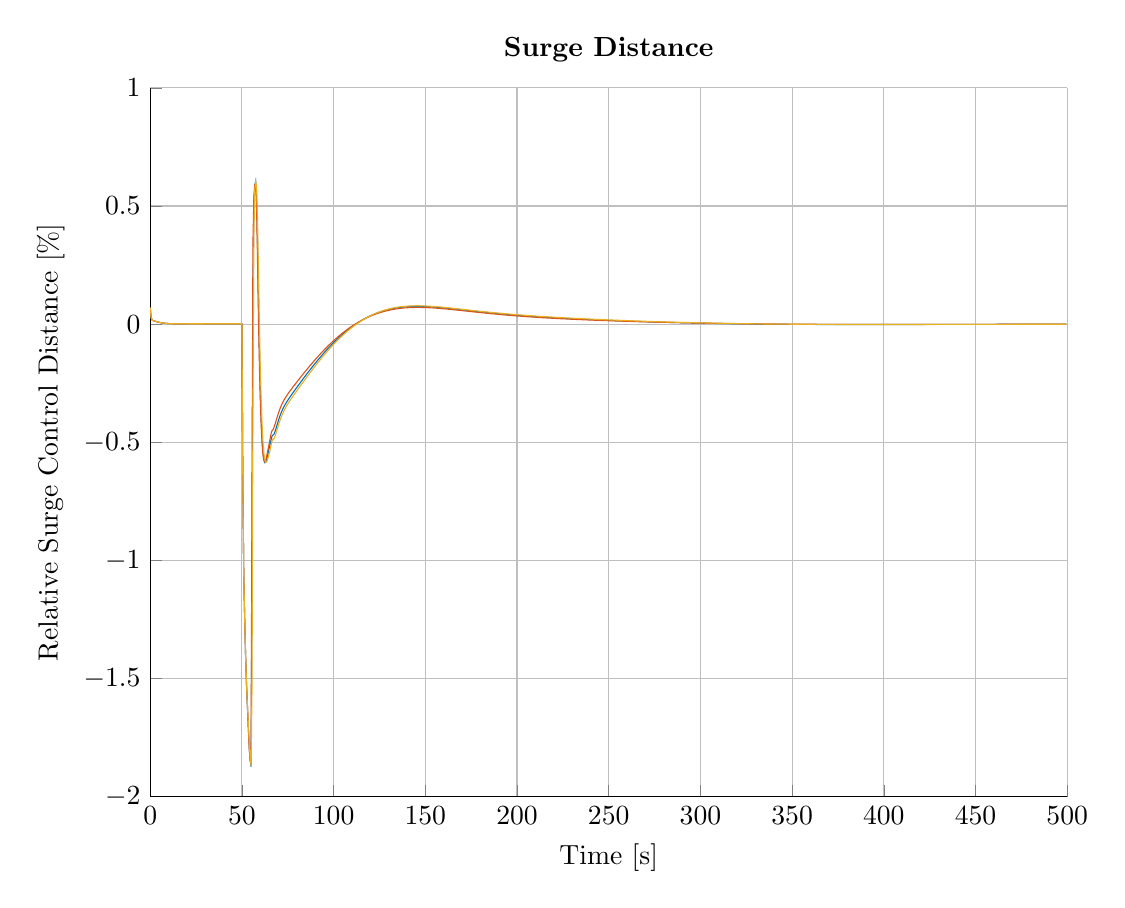
\begin{tikzpicture}

\begin{axis}[%
width=4.585in,
height=3.544in,
at={(0.769in,0.541in)},
scale only axis,
xmin=0,
xmax=500,
xlabel={Time [s]},
xmajorgrids,
ymin=-2,
ymax=1,
ylabel={Relative Surge Control Distance [\%]},
ymajorgrids,
axis background/.style={fill=white},
title style={font=\bfseries},
title={Surge Distance},
axis x line*=bottom,
axis y line*=left
]
\addplot [color=mycolor1,solid,forget plot]
  table[row sep=crcr]{%
0	0.0693700000000002\\
0.5	0.0265199999999997\\
1	0.0180300000000004\\
1.5	0.01539\\
2	0.0142600000000002\\
2.5	0.0129200000000003\\
3	0.0117099999999999\\
3.5	0.0105599999999999\\
4	0.00949000000000044\\
4.5	0.00849999999999973\\
5	0.00759000000000043\\
5.5	0.00677000000000039\\
6	0.00602999999999998\\
6.5	0.00535999999999959\\
7	0.00478000000000023\\
7.5	0.00426000000000037\\
8	0.00380999999999965\\
8.5	0.0034200000000002\\
9	0.00309000000000026\\
9.5	0.0028100000000002\\
10	0.00257000000000041\\
10.5	0.00236999999999998\\
11	0.00220999999999982\\
11.5	0.00208999999999993\\
12	0.00197999999999965\\
12.5	0.00190000000000001\\
13	0.00185000000000013\\
13.5	0.00180000000000025\\
14	0.00178000000000011\\
14.5	0.00175999999999998\\
15	0.00175000000000036\\
15.5	0.00175000000000036\\
16	0.00175999999999998\\
16.5	0.00175999999999998\\
17	0.00178000000000011\\
17.5	0.00178999999999974\\
18	0.00180000000000025\\
18.5	0.00182000000000038\\
19	0.00183\\
19.5	0.00185000000000013\\
20	0.00185999999999975\\
20.5	0.00187000000000026\\
21	0.00187999999999988\\
21.5	0.00189000000000039\\
22	0.00190000000000001\\
22.5	0.00190000000000001\\
23	0.00190999999999963\\
23.5	0.00190999999999963\\
24	0.00190999999999963\\
24.5	0.00190999999999963\\
25	0.00190999999999963\\
25.5	0.00190999999999963\\
26	0.00190999999999963\\
26.5	0.00190000000000001\\
27	0.00190000000000001\\
27.5	0.00189000000000039\\
28	0.00189000000000039\\
28.5	0.00187999999999988\\
29	0.00187000000000026\\
29.5	0.00187000000000026\\
30	0.00185999999999975\\
30.5	0.00185000000000013\\
31	0.00183999999999962\\
31.5	0.00183999999999962\\
32	0.00183\\
32.5	0.00182000000000038\\
33	0.00180999999999987\\
33.5	0.00180999999999987\\
34	0.00180000000000025\\
34.5	0.00178999999999974\\
35	0.00178999999999974\\
35.5	0.00178000000000011\\
36	0.00176999999999961\\
36.5	0.00176999999999961\\
37	0.00175999999999998\\
37.5	0.00175000000000036\\
38	0.00175000000000036\\
38.5	0.00173999999999985\\
39	0.00173999999999985\\
39.5	0.00173000000000023\\
40	0.00171999999999972\\
40.5	0.00171999999999972\\
41	0.0017100000000001\\
41.5	0.0017100000000001\\
42	0.00169999999999959\\
42.5	0.00169999999999959\\
43	0.00169999999999959\\
43.5	0.00168999999999997\\
44	0.00168999999999997\\
44.5	0.00168000000000035\\
45	0.00168000000000035\\
45.5	0.00166999999999984\\
46	0.00166999999999984\\
46.5	0.00166999999999984\\
47	0.00166000000000022\\
47.5	0.00166000000000022\\
48	0.00166000000000022\\
48.5	0.00164999999999971\\
49	0.00164999999999971\\
49.5	0.00164999999999971\\
50	0.00164000000000009\\
50.5	-0.67415\\
51	-1.0645\\
51.5	-1.24849\\
52	-1.40864\\
52.5	-1.52977\\
53	-1.62275\\
53.5	-1.70892\\
54	-1.79266\\
54.5	-1.84848\\
55	-1.87315\\
55.5	-0.9513\\
56	0.0882399999999999\\
56.5	0.50932\\
57	0.58834\\
57.5	0.60479\\
58	0.53864\\
58.5	0.34801\\
59	0.10656\\
59.5	-0.10799\\
60	-0.27716\\
60.5	-0.40193\\
61	-0.48859\\
61.5	-0.54401\\
62	-0.57478\\
62.5	-0.58661\\
63	-0.58451\\
63.5	-0.57288\\
64	-0.55556\\
64.5	-0.53597\\
65	-0.51988\\
65.5	-0.50264\\
66	-0.48649\\
66.5	-0.47203\\
67	-0.46901\\
67.5	-0.46562\\
68	-0.45617\\
68.5	-0.44403\\
69	-0.43085\\
69.5	-0.41764\\
70	-0.40499\\
70.5	-0.39325\\
71	-0.38253\\
71.5	-0.37276\\
72	-0.36386\\
72.5	-0.3557\\
73	-0.34817\\
73.5	-0.34114\\
74	-0.33453\\
74.5	-0.32823\\
75	-0.32218\\
75.5	-0.31633\\
76	-0.31062\\
76.5	-0.30502\\
77	-0.2995\\
77.5	-0.29404\\
78	-0.28862\\
78.5	-0.28324\\
79	-0.27788\\
79.5	-0.27253\\
80	-0.26721\\
80.5	-0.2619\\
81	-0.2566\\
81.5	-0.25132\\
82	-0.24606\\
82.5	-0.24081\\
83	-0.23558\\
83.5	-0.23037\\
84	-0.22518\\
84.5	-0.22001\\
85	-0.21487\\
85.5	-0.20976\\
86	-0.20467\\
86.5	-0.19962\\
87	-0.19459\\
87.5	-0.1896\\
88	-0.18465\\
88.5	-0.17972\\
89	-0.17484\\
89.5	-0.16999\\
90	-0.16518\\
90.5	-0.16041\\
91	-0.15568\\
91.5	-0.15099\\
92	-0.14634\\
92.5	-0.14173\\
93	-0.13717\\
93.5	-0.13265\\
94	-0.12817\\
94.5	-0.12374\\
95	-0.11936\\
95.5	-0.11502\\
96	-0.11073\\
96.5	-0.10648\\
97	-0.10229\\
97.5	-0.0981399999999999\\
98	-0.0940399999999997\\
98.5	-0.0899900000000002\\
99	-0.0859899999999998\\
99.5	-0.0820400000000001\\
100	-0.0781400000000003\\
100.5	-0.0742900000000004\\
101	-0.0704900000000004\\
101.5	-0.0667400000000002\\
102	-0.0630499999999996\\
102.5	-0.0594000000000001\\
103	-0.0558100000000001\\
103.5	-0.05227\\
104	-0.0487799999999998\\
104.5	-0.0453400000000004\\
105	-0.0419600000000004\\
105.5	-0.0386300000000004\\
106	-0.0353500000000002\\
106.5	-0.0321199999999999\\
107	-0.02895\\
107.5	-0.02583\\
108	-0.0227599999999999\\
108.5	-0.0197500000000002\\
109	-0.0167799999999998\\
109.5	-0.0138699999999998\\
110	-0.0110200000000003\\
110.5	-0.00821000000000005\\
111	-0.00546000000000024\\
111.5	-0.00276999999999994\\
112	-0.000119999999999898\\
112.5	0.00246999999999975\\
113	0.00502000000000002\\
113.5	0.00750999999999991\\
114	0.00994000000000028\\
114.5	0.0123300000000004\\
115	0.0146600000000001\\
115.5	0.0169499999999996\\
116	0.0191800000000004\\
116.5	0.0213599999999996\\
117	0.0234899999999998\\
117.5	0.0255700000000001\\
118	0.0275999999999996\\
118.5	0.0295800000000002\\
119	0.0315200000000004\\
119.5	0.0334000000000003\\
120	0.0352300000000003\\
120.5	0.0370200000000001\\
121	0.0387599999999999\\
121.5	0.0404499999999999\\
122	0.04209\\
122.5	0.0436899999999998\\
123	0.0452399999999997\\
123.5	0.0467399999999998\\
124	0.0481999999999996\\
124.5	0.0496100000000004\\
125	0.05098\\
125.5	0.0523100000000003\\
126	0.0535899999999998\\
126.5	0.0548299999999999\\
127	0.0560200000000002\\
127.5	0.0571799999999998\\
128	0.0582900000000004\\
128.5	0.0593599999999999\\
129	0.0603899999999999\\
129.5	0.0613799999999998\\
130	0.0623199999999997\\
130.5	0.0632400000000004\\
131	0.0641100000000003\\
131.5	0.06494\\
132	0.0657399999999999\\
132.5	0.0664999999999996\\
133	0.0672199999999998\\
133.5	0.0679100000000004\\
134	0.0685599999999997\\
134.5	0.0691800000000002\\
135	0.0697700000000001\\
135.5	0.0703199999999997\\
136	0.0708399999999996\\
136.5	0.0713200000000001\\
137	0.0717800000000004\\
137.5	0.0721999999999996\\
138	0.0725899999999999\\
138.5	0.0729600000000001\\
139	0.0732900000000001\\
139.5	0.0735999999999999\\
140	0.0738799999999999\\
140.5	0.0741300000000003\\
141	0.0743600000000004\\
141.5	0.07456\\
142	0.0747299999999997\\
142.5	0.0748800000000003\\
143	0.0750000000000002\\
143.5	0.0750999999999999\\
144	0.0751799999999996\\
144.5	0.07524\\
145	0.0752699999999997\\
145.5	0.0752899999999999\\
146	0.0752800000000002\\
146.5	0.0752499999999996\\
147	0.0752100000000002\\
147.5	0.0751400000000002\\
148	0.0750599999999997\\
148.5	0.0749599999999999\\
149	0.07484\\
149.5	0.0747\\
150	0.0745500000000003\\
150.5	0.0743900000000002\\
151	0.0742099999999999\\
151.5	0.0740100000000004\\
152	0.0738000000000003\\
152.5	0.0735799999999998\\
153	0.0733499999999996\\
153.5	0.0731000000000002\\
154	0.0728400000000002\\
154.5	0.0725699999999998\\
155	0.0722899999999997\\
155.5	0.0719900000000004\\
156	0.0716900000000003\\
156.5	0.0713800000000004\\
157	0.0710600000000001\\
157.5	0.0707300000000002\\
158	0.0704000000000002\\
158.5	0.0700500000000002\\
159	0.0697000000000001\\
159.5	0.0693400000000004\\
160	0.0689700000000002\\
160.5	0.0686\\
161	0.0682200000000002\\
161.5	0.0678400000000003\\
162	0.06745\\
162.5	0.0670599999999997\\
163	0.0666599999999997\\
163.5	0.0662599999999998\\
164	0.0658500000000002\\
164.5	0.0654500000000002\\
165	0.0650300000000001\\
165.5	0.0646199999999997\\
166	0.0641999999999996\\
166.5	0.0637800000000004\\
167	0.0633600000000003\\
167.5	0.0629299999999997\\
168	0.0625099999999996\\
168.5	0.0620799999999999\\
169	0.0616500000000002\\
169.5	0.0612199999999996\\
170	0.0607899999999999\\
170.5	0.0603600000000002\\
171	0.0599299999999996\\
171.5	0.0594999999999999\\
172	0.0590700000000002\\
172.5	0.0586399999999996\\
173	0.0582099999999999\\
173.5	0.0577800000000002\\
174	0.0573499999999996\\
174.5	0.0569199999999999\\
175	0.0564900000000002\\
175.5	0.0560700000000001\\
176	0.0556400000000004\\
176.5	0.0552200000000003\\
177	0.0547899999999997\\
177.5	0.0543699999999996\\
178	0.0539500000000004\\
178.5	0.0535300000000003\\
179	0.0531199999999998\\
179.5	0.0526999999999997\\
180	0.0522900000000002\\
180.5	0.0518799999999997\\
181	0.0514700000000001\\
181.5	0.0510700000000002\\
182	0.0506700000000002\\
182.5	0.0502599999999997\\
183	0.0498700000000003\\
183.5	0.0494700000000003\\
184	0.04908\\
184.5	0.0486800000000001\\
185	0.0482899999999997\\
185.5	0.0479099999999999\\
186	0.0475199999999996\\
186.5	0.0471399999999997\\
187	0.0467599999999999\\
187.5	0.0463899999999997\\
188	0.0460099999999999\\
188.5	0.0456399999999997\\
189	0.04528\\
189.5	0.0449099999999998\\
190	0.0445500000000001\\
190.5	0.0441900000000004\\
191	0.0438299999999998\\
191.5	0.0434799999999997\\
192	0.0431299999999997\\
192.5	0.0427799999999996\\
193	0.0424300000000004\\
193.5	0.04209\\
194	0.0417500000000004\\
194.5	0.0414099999999999\\
195	0.0410700000000004\\
195.5	0.0407400000000004\\
196	0.0404099999999996\\
196.5	0.0400799999999997\\
197	0.0397600000000002\\
197.5	0.0394300000000003\\
198	0.03911\\
198.5	0.0388000000000002\\
199	0.0384799999999998\\
199.5	0.03817\\
200	0.0378600000000002\\
200.5	0.0375500000000004\\
201	0.0372500000000002\\
201.5	0.03695\\
202	0.0366499999999998\\
202.5	0.0363499999999997\\
203	0.03606\\
203.5	0.0357599999999998\\
204	0.0354700000000001\\
204.5	0.0351900000000001\\
205	0.0349000000000004\\
205.5	0.0346200000000003\\
206	0.0343400000000003\\
206.5	0.0340600000000002\\
207	0.0337800000000001\\
207.5	0.0335099999999997\\
208	0.0332400000000002\\
208.5	0.0329699999999997\\
209	0.0327000000000002\\
209.5	0.0324299999999997\\
210	0.0321699999999998\\
210.5	0.0319099999999999\\
211	0.03165\\
211.5	0.03139\\
212	0.0311300000000001\\
212.5	0.0308799999999998\\
213	0.0306300000000004\\
213.5	0.0303800000000001\\
214	0.0301299999999998\\
214.5	0.0298800000000004\\
215	0.0296399999999997\\
215.5	0.0293900000000002\\
216	0.0291499999999996\\
216.5	0.0289099999999998\\
217	0.0286799999999996\\
217.5	0.0284399999999998\\
218	0.0282099999999996\\
218.5	0.0279699999999998\\
219	0.0277399999999997\\
219.5	0.0275100000000004\\
220	0.0272899999999998\\
220.5	0.0270599999999996\\
221	0.02684\\
221.5	0.0266099999999998\\
222	0.0263900000000001\\
222.5	0.0261699999999996\\
223	0.0259499999999999\\
223.5	0.0257399999999999\\
224	0.0255200000000002\\
224.5	0.0253100000000002\\
225	0.0250899999999996\\
225.5	0.0248799999999996\\
226	0.0246700000000004\\
226.5	0.0244600000000004\\
227	0.0242599999999999\\
227.5	0.0240499999999999\\
228	0.0238500000000004\\
228.5	0.0236400000000003\\
229	0.0234399999999999\\
229.5	0.0232400000000004\\
230	0.0230399999999999\\
230.5	0.0228400000000004\\
231	0.0226499999999996\\
231.5	0.0224500000000001\\
232	0.0222600000000002\\
232.5	0.0220599999999997\\
233	0.0218699999999998\\
233.5	0.0216799999999999\\
234	0.02149\\
234.5	0.0213000000000001\\
235	0.0211100000000002\\
235.5	0.0209299999999999\\
236	0.02074\\
236.5	0.0205599999999997\\
237	0.0203699999999998\\
237.5	0.0201900000000004\\
238	0.0200100000000001\\
238.5	0.0198299999999998\\
239	0.0196500000000004\\
239.5	0.0194700000000001\\
240	0.0193000000000003\\
240.5	0.01912\\
241	0.0189500000000002\\
241.5	0.01877\\
242	0.0186000000000002\\
242.5	0.0184300000000004\\
243	0.0182599999999997\\
243.5	0.0180899999999999\\
244	0.0179200000000002\\
244.5	0.0177500000000004\\
245	0.0175799999999997\\
245.5	0.0174200000000004\\
246	0.0172499999999998\\
246.5	0.0170899999999996\\
247	0.0169199999999998\\
247.5	0.0167599999999997\\
248	0.0166000000000004\\
248.5	0.0164400000000002\\
249	0.0162800000000001\\
249.5	0.0161199999999999\\
250	0.0159599999999998\\
};
\addplot [color=mycolor1,solid,forget plot]
  table[row sep=crcr]{%
250	0.0159599999999998\\
250.5	0.0158100000000001\\
251	0.0156499999999999\\
251.5	0.0155000000000003\\
252	0.0153400000000001\\
252.5	0.0151899999999996\\
253	0.0150300000000003\\
253.5	0.0148799999999998\\
254	0.0147300000000001\\
254.5	0.0145799999999996\\
255	0.0144299999999999\\
255.5	0.0142800000000003\\
256	0.0141400000000003\\
256.5	0.0139899999999997\\
257	0.0138400000000001\\
257.5	0.0137\\
258	0.0135500000000004\\
258.5	0.0134100000000004\\
259	0.0132700000000003\\
259.5	0.0131300000000003\\
260	0.0129900000000003\\
260.5	0.0128500000000003\\
261	0.0127100000000002\\
261.5	0.0125700000000002\\
262	0.0124300000000002\\
262.5	0.0122900000000001\\
263	0.0121599999999997\\
263.5	0.0120199999999997\\
264	0.0118900000000002\\
264.5	0.0117500000000001\\
265	0.0116199999999997\\
265.5	0.0114900000000002\\
266	0.0113599999999998\\
266.5	0.0112300000000003\\
267	0.0110999999999999\\
267.5	0.0109700000000004\\
268	0.01084\\
268.5	0.0107100000000004\\
269	0.01058\\
269.5	0.0104600000000001\\
270	0.0103299999999997\\
270.5	0.0102099999999998\\
271	0.0100800000000003\\
271.5	0.00996000000000041\\
272	0.00983999999999963\\
272.5	0.00971999999999973\\
273	0.00959999999999983\\
273.5	0.00947999999999993\\
274	0.00936000000000003\\
274.5	0.00924000000000014\\
275	0.00912000000000024\\
275.5	0.00900999999999996\\
276	0.00889000000000006\\
276.5	0.00877000000000017\\
277	0.00865999999999989\\
277.5	0.00854999999999961\\
278	0.00842999999999972\\
278.5	0.00832000000000033\\
279	0.00821000000000005\\
279.5	0.00809999999999977\\
280	0.00799000000000039\\
280.5	0.00788000000000011\\
281	0.00776999999999983\\
281.5	0.00765999999999956\\
282	0.00755000000000017\\
282.5	0.0074500000000004\\
283	0.00734000000000012\\
283.5	0.00724000000000036\\
284	0.00713000000000008\\
284.5	0.00703000000000031\\
285	0.00692999999999966\\
285.5	0.00682000000000027\\
286	0.00671999999999962\\
286.5	0.00661999999999985\\
287	0.00652000000000008\\
287.5	0.00642000000000031\\
288	0.00631999999999966\\
288.5	0.0062300000000004\\
289	0.00612999999999975\\
289.5	0.00602999999999998\\
290	0.00593999999999983\\
290.5	0.00584000000000007\\
291	0.00574999999999992\\
291.5	0.00565999999999978\\
292	0.00556000000000001\\
292.5	0.00546999999999986\\
293	0.00537999999999972\\
293.5	0.00528999999999957\\
294	0.00520000000000032\\
294.5	0.00511000000000017\\
295	0.00502000000000002\\
295.5	0.00492999999999988\\
296	0.00485000000000024\\
296.5	0.0047600000000001\\
297	0.00466999999999995\\
297.5	0.00459000000000032\\
298	0.00450999999999979\\
298.5	0.00441999999999965\\
299	0.00434000000000001\\
299.5	0.00426000000000037\\
300	0.00417000000000023\\
300.5	0.0040899999999997\\
301	0.00401000000000007\\
301.5	0.00393000000000043\\
302	0.00386000000000042\\
302.5	0.00377999999999989\\
303	0.00370000000000026\\
303.5	0.00361999999999973\\
304	0.00354999999999972\\
304.5	0.00347000000000008\\
305	0.00340000000000007\\
305.5	0.00332000000000043\\
306	0.00325000000000042\\
306.5	0.0031800000000004\\
307	0.00311000000000039\\
307.5	0.00302999999999987\\
308	0.00295999999999985\\
308.5	0.00288999999999984\\
309	0.00281999999999982\\
309.5	0.00276000000000032\\
310	0.0026900000000003\\
310.5	0.00262000000000029\\
311	0.00255000000000027\\
311.5	0.00248999999999988\\
312	0.00241999999999987\\
312.5	0.00236000000000036\\
313	0.00229000000000035\\
313.5	0.00222999999999995\\
314	0.00216999999999956\\
314.5	0.00210000000000043\\
315	0.00204000000000004\\
315.5	0.00197999999999965\\
316	0.00192000000000014\\
316.5	0.00185999999999975\\
317	0.00180000000000025\\
317.5	0.00173999999999985\\
318	0.00168999999999997\\
318.5	0.00162999999999958\\
319	0.00157000000000007\\
319.5	0.00152000000000019\\
320	0.00145999999999979\\
320.5	0.00140999999999991\\
321	0.00135000000000041\\
321.5	0.00129999999999963\\
322	0.00124999999999975\\
322.5	0.00119000000000025\\
323	0.00114000000000036\\
323.5	0.00108999999999959\\
324	0.00103999999999971\\
324.5	0.000989999999999824\\
325	0.000939999999999941\\
325.5	0.000890000000000057\\
326	0.000849999999999795\\
326.5	0.000799999999999912\\
327	0.000750000000000028\\
327.5	0.000700000000000145\\
328	0.000659999999999883\\
328.5	0.000609999999999999\\
329	0.000569999999999737\\
329.5	0.000519999999999854\\
330	0.000479999999999592\\
330.5	0.000440000000000218\\
331	0.000390000000000335\\
331.5	0.000350000000000072\\
332	0.00030999999999981\\
332.5	0.000270000000000437\\
333	0.000230000000000175\\
333.5	0.000189999999999912\\
334	0.00014999999999965\\
334.5	0.000110000000000277\\
335	7.00000000000145e-05\\
335.5	4.0000000000262e-05\\
336	0\\
336.5	-4.0000000000262e-05\\
337	-7.00000000000145e-05\\
337.5	-0.000110000000000277\\
338	-0.000140000000000029\\
338.5	-0.000180000000000291\\
339	-0.000210000000000043\\
339.5	-0.000250000000000306\\
340	-0.000280000000000058\\
340.5	-0.00030999999999981\\
341	-0.000339999999999563\\
341.5	-0.000379999999999825\\
342	-0.000409999999999577\\
342.5	-0.000440000000000218\\
343	-0.00046999999999997\\
343.5	-0.000499999999999723\\
344	-0.000530000000000364\\
344.5	-0.000549999999999606\\
345	-0.000580000000000247\\
345.5	-0.000609999999999999\\
346	-0.000639999999999752\\
346.5	-0.000659999999999883\\
347	-0.000689999999999635\\
347.5	-0.000720000000000276\\
348	-0.000740000000000407\\
348.5	-0.000770000000000159\\
349	-0.00079000000000029\\
349.5	-0.000820000000000043\\
350	-0.000840000000000174\\
350.5	-0.000860000000000305\\
351	-0.000890000000000057\\
351.5	-0.000910000000000188\\
352	-0.000930000000000319\\
352.5	-0.000949999999999562\\
353	-0.000969999999999693\\
353.5	-0.000989999999999824\\
354	-0.00100999999999996\\
354.5	-0.00103000000000009\\
355	-0.00105000000000022\\
355.5	-0.00107000000000035\\
356	-0.00108999999999959\\
356.5	-0.00110999999999972\\
357	-0.00112999999999985\\
357.5	-0.00114999999999998\\
358	-0.00115999999999961\\
358.5	-0.00117999999999974\\
359	-0.00119999999999987\\
359.5	-0.00121000000000038\\
360	-0.00122999999999962\\
360.5	-0.00124000000000013\\
361	-0.00126000000000026\\
361.5	-0.00126999999999988\\
362	-0.00129000000000001\\
362.5	-0.00129999999999963\\
363	-0.00131000000000014\\
363.5	-0.00133000000000028\\
364	-0.0013399999999999\\
364.5	-0.00135000000000041\\
365	-0.00136999999999965\\
365.5	-0.00138000000000016\\
366	-0.00138999999999978\\
366.5	-0.00140000000000029\\
367	-0.00140999999999991\\
367.5	-0.00142000000000042\\
368	-0.00143000000000004\\
368.5	-0.00143999999999966\\
369	-0.00145000000000017\\
369.5	-0.00145999999999979\\
370	-0.0014700000000003\\
370.5	-0.00147999999999993\\
371	-0.00149000000000044\\
371.5	-0.00150000000000006\\
372	-0.00150000000000006\\
372.5	-0.00150999999999968\\
373	-0.00152000000000019\\
373.5	-0.00152000000000019\\
374	-0.00152999999999981\\
374.5	-0.00154000000000032\\
375	-0.00154000000000032\\
375.5	-0.00154999999999994\\
376	-0.00155999999999956\\
376.5	-0.00155999999999956\\
377	-0.00157000000000007\\
377.5	-0.00157000000000007\\
378	-0.00157999999999969\\
378.5	-0.00157999999999969\\
379	-0.00157999999999969\\
379.5	-0.0015900000000002\\
380	-0.0015900000000002\\
380.5	-0.00159999999999982\\
381	-0.00159999999999982\\
381.5	-0.00159999999999982\\
382	-0.00159999999999982\\
382.5	-0.00161000000000033\\
383	-0.00161000000000033\\
383.5	-0.00161000000000033\\
384	-0.00161000000000033\\
384.5	-0.00161000000000033\\
385	-0.00161999999999995\\
385.5	-0.00161999999999995\\
386	-0.00161999999999995\\
386.5	-0.00161999999999995\\
387	-0.00161999999999995\\
387.5	-0.00161999999999995\\
388	-0.00161999999999995\\
388.5	-0.00161999999999995\\
389	-0.00161999999999995\\
389.5	-0.00161999999999995\\
390	-0.00161999999999995\\
390.5	-0.00161999999999995\\
391	-0.00161999999999995\\
391.5	-0.00161999999999995\\
392	-0.00161000000000033\\
392.5	-0.00161000000000033\\
393	-0.00161000000000033\\
393.5	-0.00161000000000033\\
394	-0.00161000000000033\\
394.5	-0.00161000000000033\\
395	-0.00159999999999982\\
395.5	-0.00159999999999982\\
396	-0.00159999999999982\\
396.5	-0.00159999999999982\\
397	-0.0015900000000002\\
397.5	-0.0015900000000002\\
398	-0.0015900000000002\\
398.5	-0.00157999999999969\\
399	-0.00157999999999969\\
399.5	-0.00157999999999969\\
400	-0.00157000000000007\\
400.5	-0.00157000000000007\\
401	-0.00155999999999956\\
401.5	-0.00155999999999956\\
402	-0.00155999999999956\\
402.5	-0.00154999999999994\\
403	-0.00154999999999994\\
403.5	-0.00154000000000032\\
404	-0.00154000000000032\\
404.5	-0.00152999999999981\\
405	-0.00152999999999981\\
405.5	-0.00152000000000019\\
406	-0.00152000000000019\\
406.5	-0.00150999999999968\\
407	-0.00150999999999968\\
407.5	-0.00150000000000006\\
408	-0.00150000000000006\\
408.5	-0.00149000000000044\\
409	-0.00149000000000044\\
409.5	-0.00147999999999993\\
410	-0.0014700000000003\\
410.5	-0.0014700000000003\\
411	-0.00145999999999979\\
411.5	-0.00145999999999979\\
412	-0.00145000000000017\\
412.5	-0.00143999999999966\\
413	-0.00143999999999966\\
413.5	-0.00143000000000004\\
414	-0.00142000000000042\\
414.5	-0.00142000000000042\\
415	-0.00140999999999991\\
415.5	-0.00140000000000029\\
416	-0.00140000000000029\\
416.5	-0.00138999999999978\\
417	-0.00138000000000016\\
417.5	-0.00138000000000016\\
418	-0.00136999999999965\\
418.5	-0.00136000000000003\\
419	-0.00136000000000003\\
419.5	-0.00135000000000041\\
420	-0.0013399999999999\\
420.5	-0.00133000000000028\\
421	-0.00133000000000028\\
421.5	-0.00131999999999977\\
422	-0.00131000000000014\\
422.5	-0.00129999999999963\\
423	-0.00129999999999963\\
423.5	-0.00129000000000001\\
424	-0.00128000000000039\\
424.5	-0.00126999999999988\\
425	-0.00126999999999988\\
425.5	-0.00126000000000026\\
426	-0.00124999999999975\\
426.5	-0.00124000000000013\\
427	-0.00124000000000013\\
427.5	-0.00122999999999962\\
428	-0.00122\\
428.5	-0.00121000000000038\\
429	-0.00119999999999987\\
429.5	-0.00119999999999987\\
430	-0.00119000000000025\\
430.5	-0.00117999999999974\\
431	-0.00117000000000012\\
431.5	-0.00115999999999961\\
432	-0.00115999999999961\\
432.5	-0.00114999999999998\\
433	-0.00114000000000036\\
433.5	-0.00112999999999985\\
434	-0.00112000000000023\\
434.5	-0.00112000000000023\\
435	-0.00110999999999972\\
435.5	-0.0011000000000001\\
436	-0.00108999999999959\\
436.5	-0.00107999999999997\\
437	-0.00107999999999997\\
437.5	-0.00107000000000035\\
438	-0.00105999999999984\\
438.5	-0.00105000000000022\\
439	-0.00103999999999971\\
439.5	-0.00103000000000009\\
440	-0.00103000000000009\\
440.5	-0.00101999999999958\\
441	-0.00100999999999996\\
441.5	-0.00100000000000033\\
442	-0.000989999999999824\\
442.5	-0.000989999999999824\\
443	-0.000980000000000203\\
443.5	-0.000969999999999693\\
444	-0.000960000000000072\\
444.5	-0.000949999999999562\\
445	-0.000949999999999562\\
445.5	-0.000939999999999941\\
446	-0.000930000000000319\\
446.5	-0.00091999999999981\\
447	-0.000910000000000188\\
447.5	-0.000910000000000188\\
448	-0.000899999999999679\\
448.5	-0.000890000000000057\\
449	-0.000880000000000436\\
449.5	-0.000869999999999926\\
450	-0.000869999999999926\\
450.5	-0.000860000000000305\\
451	-0.000849999999999795\\
451.5	-0.000840000000000174\\
452	-0.000829999999999664\\
452.5	-0.000829999999999664\\
453	-0.000820000000000043\\
453.5	-0.000810000000000421\\
454	-0.000799999999999912\\
454.5	-0.000799999999999912\\
455	-0.00079000000000029\\
455.5	-0.000779999999999781\\
456	-0.000770000000000159\\
456.5	-0.00075999999999965\\
457	-0.00075999999999965\\
457.5	-0.000750000000000028\\
458	-0.000740000000000407\\
458.5	-0.000729999999999897\\
459	-0.000729999999999897\\
459.5	-0.000720000000000276\\
460	-0.000709999999999766\\
460.5	-0.000700000000000145\\
461	-0.000700000000000145\\
461.5	-0.000689999999999635\\
462	-0.000680000000000014\\
462.5	-0.000680000000000014\\
463	-0.000670000000000393\\
463.5	-0.000659999999999883\\
464	-0.000650000000000261\\
464.5	-0.000650000000000261\\
465	-0.000639999999999752\\
465.5	-0.00063000000000013\\
466	-0.00063000000000013\\
466.5	-0.000619999999999621\\
467	-0.000609999999999999\\
467.5	-0.000600000000000378\\
468	-0.000600000000000378\\
468.5	-0.000589999999999868\\
469	-0.000580000000000247\\
469.5	-0.000580000000000247\\
470	-0.000569999999999737\\
470.5	-0.000560000000000116\\
471	-0.000560000000000116\\
471.5	-0.000549999999999606\\
472	-0.000539999999999985\\
472.5	-0.000539999999999985\\
473	-0.000530000000000364\\
473.5	-0.000519999999999854\\
474	-0.000519999999999854\\
474.5	-0.000510000000000232\\
475	-0.000499999999999723\\
475.5	-0.000499999999999723\\
476	-0.000490000000000101\\
476.5	-0.000490000000000101\\
477	-0.000479999999999592\\
477.5	-0.00046999999999997\\
478	-0.00046999999999997\\
478.5	-0.000460000000000349\\
479	-0.000449999999999839\\
479.5	-0.000449999999999839\\
480	-0.000440000000000218\\
480.5	-0.000440000000000218\\
481	-0.000429999999999708\\
481.5	-0.000420000000000087\\
482	-0.000420000000000087\\
482.5	-0.000409999999999577\\
483	-0.000409999999999577\\
483.5	-0.000399999999999956\\
484	-0.000399999999999956\\
484.5	-0.000390000000000335\\
485	-0.000379999999999825\\
485.5	-0.000379999999999825\\
486	-0.000370000000000203\\
486.5	-0.000370000000000203\\
487	-0.000359999999999694\\
487.5	-0.000359999999999694\\
488	-0.000350000000000072\\
488.5	-0.000350000000000072\\
489	-0.000339999999999563\\
489.5	-0.000339999999999563\\
490	-0.000329999999999941\\
490.5	-0.000329999999999941\\
491	-0.00032000000000032\\
491.5	-0.00032000000000032\\
492	-0.00030999999999981\\
492.5	-0.00030999999999981\\
493	-0.000300000000000189\\
493.5	-0.000300000000000189\\
494	-0.000289999999999679\\
494.5	-0.000289999999999679\\
495	-0.000280000000000058\\
495.5	-0.000280000000000058\\
496	-0.000270000000000437\\
496.5	-0.000270000000000437\\
497	-0.000259999999999927\\
497.5	-0.000259999999999927\\
498	-0.000250000000000306\\
498.5	-0.000250000000000306\\
499	-0.000250000000000306\\
499.5	-0.000239999999999796\\
};
\addplot [color=mycolor2,solid,forget plot]
  table[row sep=crcr]{%
0	0.0693700000000002\\
0.5	0.02644\\
1	0.0179099999999996\\
1.5	0.0152299999999999\\
2	0.0140599999999997\\
2.5	0.0126799999999996\\
3	0.0114400000000003\\
3.5	0.0102599999999997\\
4	0.00917000000000012\\
4.5	0.00816999999999979\\
5	0.00724999999999998\\
5.5	0.00642000000000031\\
6	0.00567999999999991\\
6.5	0.00502000000000002\\
7	0.00443000000000016\\
7.5	0.00393000000000043\\
8	0.00349000000000022\\
8.5	0.00311000000000039\\
9	0.00279000000000007\\
9.5	0.00251999999999963\\
10	0.00229999999999997\\
10.5	0.00211999999999968\\
11	0.00197000000000003\\
11.5	0.00185000000000013\\
12	0.00175999999999998\\
12.5	0.00169999999999959\\
13	0.00164999999999971\\
13.5	0.00161999999999995\\
14	0.00159999999999982\\
14.5	0.0015900000000002\\
15	0.0015900000000002\\
15.5	0.00159999999999982\\
16	0.00161000000000033\\
16.5	0.00161999999999995\\
17	0.00164000000000009\\
17.5	0.00164999999999971\\
18	0.00166999999999984\\
18.5	0.00168999999999997\\
19	0.00169999999999959\\
19.5	0.00171999999999972\\
20	0.00173000000000023\\
20.5	0.00173999999999985\\
21	0.00175000000000036\\
21.5	0.00175999999999998\\
22	0.00175999999999998\\
22.5	0.00176999999999961\\
23	0.00176999999999961\\
23.5	0.00176999999999961\\
24	0.00176999999999961\\
24.5	0.00176999999999961\\
25	0.00175999999999998\\
25.5	0.00175999999999998\\
26	0.00175000000000036\\
26.5	0.00175000000000036\\
27	0.00173999999999985\\
27.5	0.00173000000000023\\
28	0.00173000000000023\\
28.5	0.00171999999999972\\
29	0.0017100000000001\\
29.5	0.00169999999999959\\
30	0.00168999999999997\\
30.5	0.00168000000000035\\
31	0.00166999999999984\\
31.5	0.00166000000000022\\
32	0.00166000000000022\\
32.5	0.00164999999999971\\
33	0.00164000000000009\\
33.5	0.00162999999999958\\
34	0.00161999999999995\\
34.5	0.00161000000000033\\
35	0.00161000000000033\\
35.5	0.00159999999999982\\
36	0.0015900000000002\\
36.5	0.00157999999999969\\
37	0.00157999999999969\\
37.5	0.00157000000000007\\
38	0.00155999999999956\\
38.5	0.00155999999999956\\
39	0.00154999999999994\\
39.5	0.00154000000000032\\
40	0.00154000000000032\\
40.5	0.00152999999999981\\
41	0.00152999999999981\\
41.5	0.00152000000000019\\
42	0.00152000000000019\\
42.5	0.00150999999999968\\
43	0.00150999999999968\\
43.5	0.00150000000000006\\
44	0.00150000000000006\\
44.5	0.00149000000000044\\
45	0.00149000000000044\\
45.5	0.00147999999999993\\
46	0.00147999999999993\\
46.5	0.0014700000000003\\
47	0.0014700000000003\\
47.5	0.0014700000000003\\
48	0.00145999999999979\\
48.5	0.00145999999999979\\
49	0.00145000000000017\\
49.5	0.00145000000000017\\
50	0.00145000000000017\\
50.5	-0.67415\\
51	-1.06237\\
51.5	-1.24303\\
52	-1.39993\\
52.5	-1.51888\\
53	-1.61259\\
53.5	-1.71069\\
54	-1.80102\\
54.5	-1.84956\\
55	-1.76165\\
55.5	-0.65872\\
56	0.34617\\
56.5	0.53654\\
57	0.58873\\
57.5	0.58604\\
58	0.48594\\
58.5	0.26632\\
59	0.03111\\
59.5	-0.16736\\
60	-0.32076\\
60.5	-0.43275\\
61	-0.50874\\
61.5	-0.55495\\
62	-0.57769\\
62.5	-0.58265\\
63	-0.57491\\
63.5	-0.55894\\
64	-0.53859\\
64.5	-0.52076\\
65	-0.50044\\
65.5	-0.47929\\
66	-0.45965\\
66.5	-0.45001\\
67	-0.44632\\
67.5	-0.43688\\
68	-0.42506\\
68.5	-0.41216\\
69	-0.39917\\
69.5	-0.38646\\
70	-0.37448\\
70.5	-0.3634\\
71	-0.35325\\
71.5	-0.34399\\
72	-0.33554\\
72.5	-0.32778\\
73	-0.32061\\
73.5	-0.31393\\
74	-0.30765\\
74.5	-0.30168\\
75	-0.29595\\
75.5	-0.29042\\
76	-0.28503\\
76.5	-0.27975\\
77	-0.27456\\
77.5	-0.26943\\
78	-0.26435\\
78.5	-0.2593\\
79	-0.25428\\
79.5	-0.24929\\
80	-0.24432\\
80.5	-0.23936\\
81	-0.23442\\
81.5	-0.2295\\
82	-0.2246\\
82.5	-0.21972\\
83	-0.21486\\
83.5	-0.21002\\
84	-0.2052\\
84.5	-0.20041\\
85	-0.19565\\
85.5	-0.19091\\
86	-0.1862\\
86.5	-0.18153\\
87	-0.17688\\
87.5	-0.17226\\
88	-0.16768\\
88.5	-0.16314\\
89	-0.15863\\
89.5	-0.15415\\
90	-0.14972\\
90.5	-0.14532\\
91	-0.14096\\
91.5	-0.13664\\
92	-0.13236\\
92.5	-0.12812\\
93	-0.12392\\
93.5	-0.11977\\
94	-0.11566\\
94.5	-0.11159\\
95	-0.10756\\
95.5	-0.10358\\
96	-0.0996499999999996\\
96.5	-0.0957600000000003\\
97	-0.0919100000000004\\
97.5	-0.0881100000000004\\
98	-0.0843600000000002\\
98.5	-0.08066\\
99	-0.077\\
99.5	-0.0733800000000002\\
100	-0.06982\\
100.5	-0.0663\\
101	-0.0628299999999999\\
101.5	-0.0594099999999997\\
102	-0.0560299999999998\\
102.5	-0.0527100000000003\\
103	-0.0494300000000001\\
103.5	-0.0461999999999998\\
104	-0.0430200000000003\\
104.5	-0.0398800000000001\\
105	-0.0368000000000004\\
105.5	-0.03376\\
106	-0.03078\\
106.5	-0.0278400000000003\\
107	-0.0249499999999996\\
107.5	-0.0221099999999996\\
108	-0.0193199999999996\\
108.5	-0.0165699999999998\\
109	-0.0138800000000003\\
109.5	-0.0112300000000003\\
110	-0.00863000000000014\\
110.5	-0.00607999999999986\\
111	-0.00356999999999985\\
111.5	-0.00112000000000023\\
112	0.00129000000000001\\
112.5	0.00365000000000038\\
113	0.00595999999999997\\
113.5	0.00823000000000018\\
114	0.0104499999999996\\
114.5	0.0126200000000001\\
115	0.0147500000000003\\
115.5	0.0168299999999997\\
116	0.0188600000000001\\
116.5	0.0208500000000003\\
117	0.0227899999999996\\
117.5	0.0246899999999997\\
118	0.0265399999999998\\
118.5	0.02834\\
119	0.0301099999999996\\
119.5	0.0318300000000002\\
120	0.0335000000000001\\
120.5	0.0351299999999997\\
121	0.0367199999999999\\
121.5	0.0382699999999998\\
122	0.0397699999999999\\
122.5	0.0412299999999997\\
123	0.0426500000000001\\
123.5	0.0440300000000002\\
124	0.0453700000000001\\
124.5	0.0466699999999998\\
125	0.04793\\
125.5	0.0491400000000004\\
126	0.0503200000000001\\
126.5	0.0514599999999996\\
127	0.0525599999999997\\
127.5	0.0536300000000001\\
128	0.0546499999999996\\
128.5	0.0556400000000004\\
129	0.0566000000000004\\
129.5	0.0575099999999997\\
130	0.0583900000000002\\
130.5	0.05924\\
131	0.0600500000000004\\
131.5	0.0608300000000002\\
132	0.0615699999999997\\
132.5	0.0622800000000003\\
133	0.0629600000000003\\
133.5	0.0636000000000001\\
134	0.0642199999999997\\
134.5	0.0648\\
135	0.0653499999999996\\
135.5	0.0658700000000003\\
136	0.0663600000000004\\
136.5	0.0668199999999999\\
137	0.0672600000000001\\
137.5	0.0676600000000001\\
138	0.0680399999999999\\
138.5	0.06839\\
139	0.0687100000000003\\
139.5	0.0690099999999996\\
140	0.06928\\
140.5	0.0695300000000003\\
141	0.06975\\
141.5	0.0699500000000004\\
142	0.0701200000000002\\
142.5	0.0702800000000003\\
143	0.0704099999999999\\
143.5	0.0705099999999996\\
144	0.0705999999999998\\
144.5	0.0706699999999998\\
145	0.0707100000000001\\
145.5	0.0707399999999998\\
146	0.0707399999999998\\
146.5	0.0707300000000002\\
147	0.0707000000000004\\
147.5	0.0706499999999997\\
148	0.0705799999999996\\
148.5	0.0705\\
149	0.0704000000000002\\
149.5	0.07029\\
150	0.0701599999999996\\
150.5	0.0700099999999999\\
151	0.0698499999999997\\
151.5	0.06968\\
152	0.0694900000000001\\
152.5	0.0692899999999996\\
153	0.0690799999999996\\
153.5	0.0688500000000003\\
154	0.0686200000000001\\
154.5	0.0683699999999998\\
155	0.0681099999999999\\
155.5	0.0678400000000003\\
156	0.0675600000000003\\
156.5	0.0672699999999997\\
157	0.06698\\
157.5	0.0666700000000002\\
158	0.0663600000000004\\
158.5	0.0660299999999996\\
159	0.0656999999999996\\
159.5	0.0653699999999997\\
160	0.0650199999999996\\
160.5	0.0646699999999996\\
161	0.0643099999999999\\
161.5	0.0639500000000002\\
162	0.06358\\
162.5	0.0632099999999998\\
163	0.0628299999999999\\
163.5	0.0624500000000001\\
164	0.0620599999999998\\
164.5	0.0616700000000003\\
165	0.06128\\
165.5	0.06088\\
166	0.0604800000000001\\
166.5	0.0600800000000001\\
167	0.0596699999999997\\
167.5	0.0592600000000001\\
168	0.0588499999999996\\
168.5	0.05844\\
169	0.05802\\
169.5	0.0576100000000004\\
170	0.0571900000000003\\
170.5	0.0567700000000002\\
171	0.0563500000000001\\
171.5	0.05593\\
172	0.0555199999999996\\
172.5	0.0551000000000004\\
173	0.0546800000000003\\
173.5	0.0542600000000002\\
174	0.0538400000000001\\
174.5	0.05342\\
175	0.0529999999999999\\
175.5	0.0525799999999998\\
176	0.0521599999999998\\
176.5	0.0517500000000002\\
177	0.0513300000000001\\
177.5	0.0509199999999996\\
178	0.0505100000000001\\
178.5	0.0500999999999996\\
179	0.04969\\
179.5	0.0492800000000004\\
180	0.04887\\
180.5	0.04847\\
181	0.0480700000000001\\
181.5	0.0476700000000001\\
182	0.0472700000000001\\
182.5	0.0468799999999998\\
183	0.0464799999999999\\
183.5	0.0460900000000004\\
184	0.0457000000000001\\
184.5	0.0453099999999997\\
185	0.0449299999999999\\
185.5	0.0445500000000001\\
186	0.0441700000000003\\
186.5	0.0437900000000004\\
187	0.0434200000000002\\
187.5	0.04305\\
188	0.0426799999999998\\
188.5	0.0423099999999996\\
189	0.0419499999999999\\
189.5	0.0415900000000002\\
190	0.0412299999999997\\
190.5	0.0408799999999996\\
191	0.0405199999999999\\
191.5	0.0401699999999998\\
192	0.0398300000000003\\
192.5	0.0394800000000002\\
193	0.0391399999999997\\
193.5	0.0388000000000002\\
194	0.0384700000000002\\
194.5	0.0381299999999998\\
195	0.0377999999999998\\
195.5	0.0374800000000004\\
196	0.0371499999999996\\
196.5	0.0368300000000001\\
197	0.0365099999999998\\
197.5	0.0362\\
198	0.0358799999999997\\
198.5	0.0355699999999999\\
199	0.0352699999999997\\
199.5	0.0349599999999999\\
200	0.0346599999999997\\
200.5	0.0343600000000004\\
201	0.0340600000000002\\
201.5	0.0337699999999996\\
202	0.03348\\
202.5	0.0331900000000003\\
203	0.0328999999999997\\
203.5	0.0326199999999996\\
204	0.03233\\
204.5	0.0320600000000004\\
205	0.0317800000000004\\
205.5	0.0315099999999999\\
206	0.0312299999999999\\
206.5	0.0309699999999999\\
207	0.0307000000000004\\
207.5	0.0304399999999996\\
208	0.03017\\
208.5	0.0299199999999997\\
209	0.0296599999999998\\
209.5	0.0293999999999999\\
210	0.0291499999999996\\
210.5	0.0289000000000001\\
211	0.0286499999999998\\
211.5	0.02841\\
212	0.0281599999999997\\
212.5	0.0279199999999999\\
213	0.0276800000000001\\
213.5	0.02745\\
214	0.0272100000000002\\
214.5	0.02698\\
215	0.0267499999999998\\
215.5	0.0265199999999997\\
216	0.0262900000000004\\
216.5	0.0260699999999998\\
217	0.0258399999999996\\
217.5	0.02562\\
218	0.0254000000000003\\
218.5	0.0251900000000003\\
219	0.0249699999999997\\
219.5	0.0247599999999997\\
220	0.0245499999999996\\
220.5	0.0243399999999996\\
221	0.0241300000000004\\
221.5	0.0239200000000004\\
222	0.02372\\
222.5	0.0235099999999999\\
223	0.0233100000000004\\
223.5	0.02311\\
224	0.0229100000000004\\
224.5	0.0227199999999996\\
225	0.0225200000000001\\
225.5	0.0223300000000002\\
226	0.0221400000000003\\
226.5	0.0219500000000004\\
227	0.0217599999999996\\
227.5	0.0215699999999996\\
228	0.0213799999999997\\
228.5	0.0212000000000003\\
229	0.02102\\
229.5	0.0208300000000001\\
230	0.0206499999999998\\
230.5	0.0204700000000004\\
231	0.0202999999999998\\
231.5	0.0201200000000004\\
232	0.0199499999999997\\
232.5	0.0197700000000003\\
233	0.0195999999999996\\
233.5	0.0194299999999998\\
234	0.0192600000000001\\
234.5	0.0190900000000003\\
235	0.0189199999999996\\
235.5	0.0187600000000003\\
236	0.0185899999999997\\
236.5	0.0184300000000004\\
237	0.0182599999999997\\
237.5	0.0180999999999996\\
238	0.0179400000000003\\
238.5	0.0177800000000001\\
239	0.01762\\
239.5	0.0174700000000003\\
240	0.0173100000000002\\
240.5	0.0171599999999996\\
241	0.0170000000000003\\
241.5	0.0168499999999998\\
242	0.0167000000000002\\
242.5	0.0165499999999996\\
243	0.0164\\
243.5	0.0162500000000003\\
244	0.0160999999999998\\
244.5	0.0159500000000001\\
245	0.0158100000000001\\
245.5	0.0156599999999996\\
246	0.0155200000000004\\
246.5	0.0153800000000004\\
247	0.0152400000000004\\
247.5	0.0151000000000003\\
248	0.0149600000000003\\
248.5	0.0148200000000003\\
249	0.0146800000000002\\
249.5	0.0145400000000002\\
250	0.0144000000000002\\
};
\addplot [color=mycolor2,solid,forget plot]
  table[row sep=crcr]{%
250	0.0144000000000002\\
250.5	0.0142699999999998\\
251	0.0141299999999998\\
251.5	0.0140000000000002\\
252	0.0138699999999998\\
252.5	0.0137299999999998\\
253	0.0136000000000003\\
253.5	0.0134699999999999\\
254	0.0133400000000004\\
254.5	0.0132099999999999\\
255	0.01309\\
255.5	0.0129599999999996\\
256	0.0128300000000001\\
256.5	0.0127100000000002\\
257	0.0125799999999998\\
257.5	0.0124599999999999\\
258	0.01234\\
258.5	0.0122099999999996\\
259	0.0120899999999997\\
259.5	0.0119699999999998\\
260	0.0118499999999999\\
260.5	0.01173\\
261	0.0116100000000001\\
261.5	0.0114900000000002\\
262	0.0113799999999999\\
262.5	0.01126\\
263	0.0111400000000001\\
263.5	0.0110299999999999\\
264	0.0109199999999996\\
264.5	0.0107999999999997\\
265	0.0106900000000003\\
265.5	0.01058\\
266	0.0104699999999998\\
266.5	0.0103499999999999\\
267	0.0102399999999996\\
267.5	0.0101300000000002\\
268	0.0100300000000004\\
268.5	0.00992000000000015\\
269	0.00980999999999987\\
269.5	0.0096999999999996\\
270	0.00959999999999983\\
270.5	0.00949000000000044\\
271	0.00938999999999979\\
271.5	0.0092800000000004\\
272	0.00917999999999974\\
272.5	0.00907999999999998\\
273	0.00898000000000021\\
273.5	0.00886999999999993\\
274	0.00877000000000017\\
274.5	0.0086700000000004\\
275	0.00856999999999974\\
275.5	0.0084799999999996\\
276	0.00837999999999983\\
276.5	0.00828000000000007\\
277	0.0081800000000003\\
277.5	0.00809000000000015\\
278	0.00799000000000039\\
278.5	0.00790000000000024\\
279	0.00779999999999959\\
279.5	0.00771000000000033\\
280	0.00760999999999967\\
280.5	0.00752000000000042\\
281	0.00743000000000027\\
281.5	0.00734000000000012\\
282	0.00724999999999998\\
282.5	0.00715999999999983\\
283	0.00706999999999969\\
283.5	0.00698000000000043\\
284	0.00689000000000028\\
284.5	0.00680000000000014\\
285	0.00671999999999962\\
285.5	0.00663000000000036\\
286	0.00654000000000021\\
286.5	0.00645999999999969\\
287	0.00637000000000043\\
287.5	0.00628999999999991\\
288	0.00621000000000027\\
288.5	0.00612000000000013\\
289	0.0060399999999996\\
289.5	0.00595999999999997\\
290	0.00588000000000033\\
290.5	0.00579999999999981\\
291	0.00572000000000017\\
291.5	0.00563999999999965\\
292	0.00556000000000001\\
292.5	0.00548000000000037\\
293	0.00539999999999985\\
293.5	0.00532999999999983\\
294	0.0052500000000002\\
294.5	0.00516999999999967\\
295	0.00509999999999966\\
295.5	0.00502000000000002\\
296	0.00495000000000001\\
296.5	0.00487000000000037\\
297	0.00480000000000036\\
297.5	0.00473000000000035\\
298	0.00466000000000033\\
298.5	0.00457999999999981\\
299	0.00450999999999979\\
299.5	0.00443999999999978\\
300	0.00436999999999976\\
300.5	0.00429999999999975\\
301	0.00422999999999973\\
301.5	0.00417000000000023\\
302	0.00410000000000021\\
302.5	0.0040300000000002\\
303	0.00396000000000019\\
303.5	0.00389999999999979\\
304	0.00382999999999978\\
304.5	0.00377000000000027\\
305	0.00370000000000026\\
305.5	0.00363999999999987\\
306	0.00358000000000036\\
306.5	0.00351000000000035\\
307	0.00344999999999995\\
307.5	0.00338999999999956\\
308	0.00333000000000006\\
308.5	0.00326999999999966\\
309	0.00319999999999965\\
309.5	0.00314000000000014\\
310	0.00309000000000026\\
310.5	0.00302999999999987\\
311	0.00297000000000036\\
311.5	0.00290999999999997\\
312	0.00284999999999958\\
312.5	0.00279999999999969\\
313	0.00274000000000019\\
313.5	0.00267999999999979\\
314	0.00262999999999991\\
314.5	0.00257000000000041\\
315	0.00251999999999963\\
315.5	0.00246999999999975\\
316	0.00241000000000025\\
316.5	0.00236000000000036\\
317	0.00230999999999959\\
317.5	0.00225000000000009\\
318	0.0022000000000002\\
318.5	0.00215000000000032\\
319	0.00210000000000043\\
319.5	0.00204999999999966\\
320	0.00199999999999978\\
320.5	0.0019499999999999\\
321	0.00190999999999963\\
321.5	0.00185999999999975\\
322	0.00180999999999987\\
322.5	0.00175999999999998\\
323	0.00171999999999972\\
323.5	0.00166999999999984\\
324	0.00161999999999995\\
324.5	0.00157999999999969\\
325	0.00152999999999981\\
325.5	0.00149000000000044\\
326	0.00145000000000017\\
326.5	0.00140000000000029\\
327	0.00136000000000003\\
327.5	0.00131999999999977\\
328	0.00126999999999988\\
328.5	0.00122999999999962\\
329	0.00119000000000025\\
329.5	0.00114999999999998\\
330	0.00110999999999972\\
330.5	0.00107000000000035\\
331	0.00103000000000009\\
331.5	0.000989999999999824\\
332	0.000949999999999562\\
332.5	0.00091999999999981\\
333	0.000880000000000436\\
333.5	0.000840000000000174\\
334	0.000799999999999912\\
334.5	0.000770000000000159\\
335	0.000729999999999897\\
335.5	0.000700000000000145\\
336	0.000659999999999883\\
336.5	0.00063000000000013\\
337	0.000589999999999868\\
337.5	0.000560000000000116\\
338	0.000519999999999854\\
338.5	0.000490000000000101\\
339	0.000460000000000349\\
339.5	0.000429999999999708\\
340	0.000390000000000335\\
340.5	0.000359999999999694\\
341	0.000329999999999941\\
341.5	0.000300000000000189\\
342	0.000270000000000437\\
342.5	0.000239999999999796\\
343	0.000210000000000043\\
343.5	0.000180000000000291\\
344	0.00014999999999965\\
344.5	0.000119999999999898\\
345	9.99999999997669e-05\\
345.5	7.00000000000145e-05\\
346	4.0000000000262e-05\\
346.5	2.0000000000131e-05\\
347	-9.99999999962142e-06\\
347.5	-4.0000000000262e-05\\
348	-6.00000000003931e-05\\
348.5	-9.00000000001455e-05\\
349	-0.000110000000000277\\
349.5	-0.000140000000000029\\
350	-0.00016000000000016\\
350.5	-0.000189999999999912\\
351	-0.000210000000000043\\
351.5	-0.000230000000000175\\
352	-0.000259999999999927\\
352.5	-0.000280000000000058\\
353	-0.000300000000000189\\
353.5	-0.00032000000000032\\
354	-0.000350000000000072\\
354.5	-0.000370000000000203\\
355	-0.000390000000000335\\
355.5	-0.000409999999999577\\
356	-0.000429999999999708\\
356.5	-0.000449999999999839\\
357	-0.00046999999999997\\
357.5	-0.000490000000000101\\
358	-0.000510000000000232\\
358.5	-0.000530000000000364\\
359	-0.000539999999999985\\
359.5	-0.000560000000000116\\
360	-0.000580000000000247\\
360.5	-0.000600000000000378\\
361	-0.000609999999999999\\
361.5	-0.00063000000000013\\
362	-0.000650000000000261\\
362.5	-0.000659999999999883\\
363	-0.000680000000000014\\
363.5	-0.000700000000000145\\
364	-0.000709999999999766\\
364.5	-0.000729999999999897\\
365	-0.000740000000000407\\
365.5	-0.00075999999999965\\
366	-0.000770000000000159\\
366.5	-0.000779999999999781\\
367	-0.000799999999999912\\
367.5	-0.000810000000000421\\
368	-0.000820000000000043\\
368.5	-0.000840000000000174\\
369	-0.000849999999999795\\
369.5	-0.000860000000000305\\
370	-0.000869999999999926\\
370.5	-0.000890000000000057\\
371	-0.000899999999999679\\
371.5	-0.000910000000000188\\
372	-0.00091999999999981\\
372.5	-0.000930000000000319\\
373	-0.000939999999999941\\
373.5	-0.000949999999999562\\
374	-0.000960000000000072\\
374.5	-0.000969999999999693\\
375	-0.000980000000000203\\
375.5	-0.000989999999999824\\
376	-0.00100000000000033\\
376.5	-0.00100999999999996\\
377	-0.00101999999999958\\
377.5	-0.00103000000000009\\
378	-0.00103000000000009\\
378.5	-0.00103999999999971\\
379	-0.00105000000000022\\
379.5	-0.00105999999999984\\
380	-0.00105999999999984\\
380.5	-0.00107000000000035\\
381	-0.00107999999999997\\
381.5	-0.00108999999999959\\
382	-0.00108999999999959\\
382.5	-0.0011000000000001\\
383	-0.0011000000000001\\
383.5	-0.00110999999999972\\
384	-0.00112000000000023\\
384.5	-0.00112000000000023\\
385	-0.00112999999999985\\
385.5	-0.00112999999999985\\
386	-0.00114000000000036\\
386.5	-0.00114000000000036\\
387	-0.00114999999999998\\
387.5	-0.00114999999999998\\
388	-0.00114999999999998\\
388.5	-0.00115999999999961\\
389	-0.00115999999999961\\
389.5	-0.00117000000000012\\
390	-0.00117000000000012\\
390.5	-0.00117000000000012\\
391	-0.00117999999999974\\
391.5	-0.00117999999999974\\
392	-0.00117999999999974\\
392.5	-0.00117999999999974\\
393	-0.00119000000000025\\
393.5	-0.00119000000000025\\
394	-0.00119000000000025\\
394.5	-0.00119000000000025\\
395	-0.00119999999999987\\
395.5	-0.00119999999999987\\
396	-0.00119999999999987\\
396.5	-0.00119999999999987\\
397	-0.00119999999999987\\
397.5	-0.00119999999999987\\
398	-0.00119999999999987\\
398.5	-0.00119999999999987\\
399	-0.00119999999999987\\
399.5	-0.00121000000000038\\
400	-0.00121000000000038\\
400.5	-0.00121000000000038\\
401	-0.00121000000000038\\
401.5	-0.00121000000000038\\
402	-0.00121000000000038\\
402.5	-0.00121000000000038\\
403	-0.00121000000000038\\
403.5	-0.00121000000000038\\
404	-0.00119999999999987\\
404.5	-0.00119999999999987\\
405	-0.00119999999999987\\
405.5	-0.00119999999999987\\
406	-0.00119999999999987\\
406.5	-0.00119999999999987\\
407	-0.00119999999999987\\
407.5	-0.00119999999999987\\
408	-0.00119999999999987\\
408.5	-0.00119000000000025\\
409	-0.00119000000000025\\
409.5	-0.00119000000000025\\
410	-0.00119000000000025\\
410.5	-0.00119000000000025\\
411	-0.00117999999999974\\
411.5	-0.00117999999999974\\
412	-0.00117999999999974\\
412.5	-0.00117999999999974\\
413	-0.00117999999999974\\
413.5	-0.00117000000000012\\
414	-0.00117000000000012\\
414.5	-0.00117000000000012\\
415	-0.00115999999999961\\
415.5	-0.00115999999999961\\
416	-0.00115999999999961\\
416.5	-0.00115999999999961\\
417	-0.00114999999999998\\
417.5	-0.00114999999999998\\
418	-0.00114999999999998\\
418.5	-0.00114000000000036\\
419	-0.00114000000000036\\
419.5	-0.00114000000000036\\
420	-0.00112999999999985\\
420.5	-0.00112999999999985\\
421	-0.00112000000000023\\
421.5	-0.00112000000000023\\
422	-0.00112000000000023\\
422.5	-0.00110999999999972\\
423	-0.00110999999999972\\
423.5	-0.0011000000000001\\
424	-0.0011000000000001\\
424.5	-0.0011000000000001\\
425	-0.00108999999999959\\
425.5	-0.00108999999999959\\
426	-0.00107999999999997\\
426.5	-0.00107999999999997\\
427	-0.00107999999999997\\
427.5	-0.00107000000000035\\
428	-0.00107000000000035\\
428.5	-0.00105999999999984\\
429	-0.00105999999999984\\
429.5	-0.00105000000000022\\
430	-0.00105000000000022\\
430.5	-0.00103999999999971\\
431	-0.00103999999999971\\
431.5	-0.00103000000000009\\
432	-0.00103000000000009\\
432.5	-0.00101999999999958\\
433	-0.00101999999999958\\
433.5	-0.00100999999999996\\
434	-0.00100999999999996\\
434.5	-0.00100000000000033\\
435	-0.00100000000000033\\
435.5	-0.000989999999999824\\
436	-0.000989999999999824\\
436.5	-0.000980000000000203\\
437	-0.000980000000000203\\
437.5	-0.000969999999999693\\
438	-0.000969999999999693\\
438.5	-0.000960000000000072\\
439	-0.000960000000000072\\
439.5	-0.000949999999999562\\
440	-0.000949999999999562\\
440.5	-0.000939999999999941\\
441	-0.000939999999999941\\
441.5	-0.000930000000000319\\
442	-0.00091999999999981\\
442.5	-0.00091999999999981\\
443	-0.000910000000000188\\
443.5	-0.000910000000000188\\
444	-0.000899999999999679\\
444.5	-0.000899999999999679\\
445	-0.000890000000000057\\
445.5	-0.000890000000000057\\
446	-0.000880000000000436\\
446.5	-0.000880000000000436\\
447	-0.000869999999999926\\
447.5	-0.000860000000000305\\
448	-0.000860000000000305\\
448.5	-0.000849999999999795\\
449	-0.000849999999999795\\
449.5	-0.000840000000000174\\
450	-0.000840000000000174\\
450.5	-0.000829999999999664\\
451	-0.000820000000000043\\
451.5	-0.000820000000000043\\
452	-0.000810000000000421\\
452.5	-0.000810000000000421\\
453	-0.000799999999999912\\
453.5	-0.000799999999999912\\
454	-0.00079000000000029\\
454.5	-0.00079000000000029\\
455	-0.000779999999999781\\
455.5	-0.000770000000000159\\
456	-0.000770000000000159\\
456.5	-0.00075999999999965\\
457	-0.00075999999999965\\
457.5	-0.000750000000000028\\
458	-0.000750000000000028\\
458.5	-0.000740000000000407\\
459	-0.000729999999999897\\
459.5	-0.000729999999999897\\
460	-0.000720000000000276\\
460.5	-0.000720000000000276\\
461	-0.000709999999999766\\
461.5	-0.000709999999999766\\
462	-0.000700000000000145\\
462.5	-0.000700000000000145\\
463	-0.000689999999999635\\
463.5	-0.000680000000000014\\
464	-0.000680000000000014\\
464.5	-0.000670000000000393\\
465	-0.000670000000000393\\
465.5	-0.000659999999999883\\
466	-0.000659999999999883\\
466.5	-0.000650000000000261\\
467	-0.000650000000000261\\
467.5	-0.000639999999999752\\
468	-0.00063000000000013\\
468.5	-0.00063000000000013\\
469	-0.000619999999999621\\
469.5	-0.000619999999999621\\
470	-0.000609999999999999\\
470.5	-0.000609999999999999\\
471	-0.000600000000000378\\
471.5	-0.000600000000000378\\
472	-0.000589999999999868\\
472.5	-0.000589999999999868\\
473	-0.000580000000000247\\
473.5	-0.000580000000000247\\
474	-0.000569999999999737\\
474.5	-0.000569999999999737\\
475	-0.000560000000000116\\
475.5	-0.000549999999999606\\
476	-0.000549999999999606\\
476.5	-0.000539999999999985\\
477	-0.000539999999999985\\
477.5	-0.000530000000000364\\
478	-0.000530000000000364\\
478.5	-0.000519999999999854\\
479	-0.000519999999999854\\
479.5	-0.000510000000000232\\
480	-0.000510000000000232\\
480.5	-0.000499999999999723\\
481	-0.000499999999999723\\
481.5	-0.000490000000000101\\
482	-0.000490000000000101\\
482.5	-0.000479999999999592\\
483	-0.000479999999999592\\
483.5	-0.00046999999999997\\
484	-0.00046999999999997\\
484.5	-0.000460000000000349\\
485	-0.000460000000000349\\
485.5	-0.000460000000000349\\
486	-0.000449999999999839\\
486.5	-0.000449999999999839\\
487	-0.000440000000000218\\
487.5	-0.000440000000000218\\
488	-0.000429999999999708\\
488.5	-0.000429999999999708\\
489	-0.000420000000000087\\
489.5	-0.000420000000000087\\
490	-0.000409999999999577\\
490.5	-0.000409999999999577\\
491	-0.000399999999999956\\
491.5	-0.000399999999999956\\
492	-0.000399999999999956\\
492.5	-0.000390000000000335\\
493	-0.000390000000000335\\
493.5	-0.000379999999999825\\
494	-0.000379999999999825\\
494.5	-0.000370000000000203\\
495	-0.000370000000000203\\
495.5	-0.000359999999999694\\
496	-0.000359999999999694\\
496.5	-0.000359999999999694\\
497	-0.000350000000000072\\
497.5	-0.000350000000000072\\
498	-0.000339999999999563\\
498.5	-0.000339999999999563\\
499	-0.000339999999999563\\
499.5	-0.000329999999999941\\
};
\addplot [color=mycolor3,solid,forget plot]
  table[row sep=crcr]{%
0	0.0693700000000002\\
0.5	0.0265700000000004\\
1	0.0180400000000001\\
1.5	0.0153600000000003\\
2	0.0141900000000001\\
2.5	0.01281\\
3	0.0115699999999999\\
3.5	0.0103900000000001\\
4	0.00929000000000002\\
4.5	0.00828000000000007\\
5	0.00736000000000026\\
5.5	0.00652000000000008\\
6	0.00577000000000005\\
6.5	0.00509999999999966\\
7	0.0045200000000003\\
7.5	0.00399999999999956\\
8	0.00356000000000023\\
8.5	0.0031699999999999\\
9	0.00284999999999958\\
9.5	0.00257000000000041\\
10	0.00234999999999985\\
10.5	0.00215999999999994\\
11	0.00201000000000029\\
11.5	0.00189000000000039\\
12	0.00180000000000025\\
12.5	0.00173000000000023\\
13	0.00168000000000035\\
13.5	0.00164000000000009\\
14	0.00161999999999995\\
14.5	0.00161000000000033\\
15	0.00161000000000033\\
15.5	0.00161000000000033\\
16	0.00161999999999995\\
16.5	0.00162999999999958\\
17	0.00164999999999971\\
17.5	0.00166999999999984\\
18	0.00168000000000035\\
18.5	0.00169999999999959\\
19	0.00171999999999972\\
19.5	0.00173000000000023\\
20	0.00175000000000036\\
20.5	0.00175999999999998\\
21	0.00176999999999961\\
21.5	0.00178000000000011\\
22	0.00178999999999974\\
22.5	0.00180000000000025\\
23	0.00180000000000025\\
23.5	0.00180999999999987\\
24	0.00180999999999987\\
24.5	0.00180999999999987\\
25	0.00180999999999987\\
25.5	0.00180999999999987\\
26	0.00180999999999987\\
26.5	0.00180000000000025\\
27	0.00180000000000025\\
27.5	0.00180000000000025\\
28	0.00178999999999974\\
28.5	0.00178999999999974\\
29	0.00178000000000011\\
29.5	0.00176999999999961\\
30	0.00176999999999961\\
30.5	0.00175999999999998\\
31	0.00175999999999998\\
31.5	0.00175000000000036\\
32	0.00173999999999985\\
32.5	0.00173999999999985\\
33	0.00173000000000023\\
33.5	0.00173000000000023\\
34	0.00171999999999972\\
34.5	0.0017100000000001\\
35	0.0017100000000001\\
35.5	0.00169999999999959\\
36	0.00169999999999959\\
36.5	0.00168999999999997\\
37	0.00168999999999997\\
37.5	0.00168000000000035\\
38	0.00168000000000035\\
38.5	0.00166999999999984\\
39	0.00166999999999984\\
39.5	0.00166000000000022\\
40	0.00166000000000022\\
40.5	0.00164999999999971\\
41	0.00164999999999971\\
41.5	0.00164999999999971\\
42	0.00164000000000009\\
42.5	0.00164000000000009\\
43	0.00164000000000009\\
43.5	0.00162999999999958\\
44	0.00162999999999958\\
44.5	0.00162999999999958\\
45	0.00161999999999995\\
45.5	0.00161999999999995\\
46	0.00161999999999995\\
46.5	0.00161000000000033\\
47	0.00161000000000033\\
47.5	0.00161000000000033\\
48	0.00161000000000033\\
48.5	0.00159999999999982\\
49	0.00159999999999982\\
49.5	0.00159999999999982\\
50	0.00159999999999982\\
50.5	-0.67404\\
51	-1.06278\\
51.5	-1.24484\\
52	-1.40333\\
52.5	-1.52325\\
53	-1.61542\\
53.5	-1.68774\\
54	-1.7737\\
54.5	-1.83676\\
55	-1.87006\\
55.5	-1.53907\\
56	-0.36041\\
56.5	0.36855\\
57	0.56805\\
57.5	0.60364\\
58	0.57701\\
58.5	0.44468\\
59	0.23119\\
59.5	0.0104499999999996\\
60	-0.17608\\
60.5	-0.32107\\
61	-0.42753\\
61.5	-0.50133\\
62	-0.54856\\
62.5	-0.57476\\
63	-0.5848\\
63.5	-0.58289\\
64	-0.57279\\
64.5	-0.55795\\
65	-0.54423\\
65.5	-0.52671\\
66	-0.50881\\
66.5	-0.49202\\
67	-0.48764\\
67.5	-0.48425\\
68	-0.47531\\
68.5	-0.46374\\
69	-0.45096\\
69.5	-0.43793\\
70	-0.42521\\
70.5	-0.4132\\
71	-0.40204\\
71.5	-0.39175\\
72	-0.38227\\
72.5	-0.37354\\
73	-0.36545\\
73.5	-0.35791\\
74	-0.35084\\
74.5	-0.34414\\
75	-0.33776\\
75.5	-0.33162\\
76	-0.32567\\
76.5	-0.31988\\
77	-0.3142\\
77.5	-0.30861\\
78	-0.30309\\
78.5	-0.29761\\
79	-0.29217\\
79.5	-0.28675\\
80	-0.28135\\
80.5	-0.27597\\
81	-0.2706\\
81.5	-0.26523\\
82	-0.25988\\
82.5	-0.25454\\
83	-0.2492\\
83.5	-0.24388\\
84	-0.23858\\
84.5	-0.23329\\
85	-0.22802\\
85.5	-0.22277\\
86	-0.21754\\
86.5	-0.21233\\
87	-0.20715\\
87.5	-0.202\\
88	-0.19687\\
88.5	-0.19178\\
89	-0.18671\\
89.5	-0.18168\\
90	-0.17668\\
90.5	-0.17172\\
91	-0.1668\\
91.5	-0.16191\\
92	-0.15706\\
92.5	-0.15226\\
93	-0.14749\\
93.5	-0.14276\\
94	-0.13808\\
94.5	-0.13344\\
95	-0.12884\\
95.5	-0.12429\\
96	-0.11978\\
96.5	-0.11532\\
97	-0.11091\\
97.5	-0.10655\\
98	-0.10223\\
98.5	-0.0979599999999996\\
99	-0.0937400000000004\\
99.5	-0.0895799999999998\\
100	-0.0854600000000003\\
100.5	-0.0813899999999999\\
101	-0.0773700000000002\\
101.5	-0.07341\\
102	-0.0694999999999997\\
102.5	-0.0656400000000001\\
103	-0.0618299999999996\\
103.5	-0.0580800000000004\\
104	-0.0543800000000001\\
104.5	-0.0507299999999997\\
105	-0.0471399999999997\\
105.5	-0.0435999999999996\\
106	-0.0401199999999999\\
106.5	-0.0366900000000001\\
107	-0.0333199999999998\\
107.5	-0.0300000000000002\\
108	-0.0267400000000002\\
108.5	-0.0235300000000001\\
109	-0.0203699999999998\\
109.5	-0.0172800000000004\\
110	-0.0142300000000004\\
110.5	-0.0112500000000004\\
111	-0.00832000000000033\\
111.5	-0.00544000000000011\\
112	-0.00262000000000029\\
112.5	0.00014999999999965\\
113	0.00286000000000008\\
113.5	0.00551000000000013\\
114	0.00811000000000028\\
114.5	0.0106599999999997\\
115	0.0131500000000004\\
115.5	0.0155799999999999\\
116	0.01797\\
116.5	0.0202900000000001\\
117	0.02257\\
117.5	0.0247900000000003\\
118	0.0269599999999999\\
118.5	0.0290699999999999\\
119	0.0311300000000001\\
119.5	0.0331400000000004\\
120	0.0350999999999999\\
120.5	0.0369999999999999\\
121	0.0388599999999997\\
121.5	0.0406599999999999\\
122	0.0424100000000003\\
122.5	0.0441099999999999\\
123	0.0457700000000001\\
123.5	0.0473699999999999\\
124	0.0489300000000004\\
124.5	0.0504300000000004\\
125	0.0518900000000002\\
125.5	0.0533000000000001\\
126	0.0546600000000002\\
126.5	0.0559799999999999\\
127	0.0572499999999998\\
127.5	0.0584800000000003\\
128	0.05966\\
128.5	0.0608000000000004\\
129	0.06189\\
129.5	0.0629499999999998\\
130	0.0639500000000002\\
130.5	0.0649199999999999\\
131	0.0658500000000002\\
131.5	0.0667299999999997\\
132	0.0675800000000004\\
132.5	0.0683800000000003\\
133	0.0691499999999996\\
133.5	0.0698800000000004\\
134	0.07057\\
134.5	0.0712200000000003\\
135	0.0718399999999999\\
135.5	0.0724200000000002\\
136	0.0729699999999998\\
136.5	0.0734899999999996\\
137	0.0739700000000001\\
137.5	0.0744100000000003\\
138	0.0748300000000004\\
138.5	0.0752100000000002\\
139	0.0755699999999999\\
139.5	0.0758900000000002\\
140	0.0761799999999999\\
140.5	0.0764500000000004\\
141	0.0766900000000001\\
141.5	0.0769000000000002\\
142	0.0770799999999996\\
142.5	0.0772399999999998\\
143	0.0773700000000002\\
143.5	0.0774699999999999\\
144	0.0775600000000001\\
144.5	0.0776199999999996\\
145	0.0776500000000002\\
145.5	0.0776700000000003\\
146	0.0776599999999998\\
146.5	0.0776300000000001\\
147	0.0775899999999998\\
147.5	0.0775199999999998\\
148	0.0774299999999997\\
148.5	0.0773299999999999\\
149	0.07721\\
149.5	0.07707\\
150	0.0769099999999998\\
150.5	0.07674\\
151	0.0765500000000001\\
151.5	0.0763499999999997\\
152	0.0761399999999997\\
152.5	0.0759100000000004\\
153	0.0756600000000001\\
153.5	0.0754099999999998\\
154	0.0751400000000002\\
154.5	0.0748600000000001\\
155	0.0745800000000001\\
155.5	0.0742799999999999\\
156	0.0739700000000001\\
156.5	0.0736499999999998\\
157	0.0733199999999998\\
157.5	0.0729800000000003\\
158	0.0726399999999998\\
158.5	0.0722800000000001\\
159	0.0719200000000004\\
159.5	0.0715599999999998\\
160	0.07118\\
160.5	0.0708000000000002\\
161	0.0704200000000004\\
161.5	0.07003\\
162	0.0696300000000001\\
162.5	0.0692300000000001\\
163	0.0688300000000002\\
163.5	0.0684199999999997\\
164	0.0680100000000001\\
164.5	0.06759\\
165	0.06717\\
165.5	0.0667499999999999\\
166	0.0663299999999998\\
166.5	0.0659000000000001\\
167	0.0654700000000004\\
167.5	0.0650500000000003\\
168	0.0646100000000001\\
168.5	0.0641800000000003\\
169	0.0637499999999998\\
169.5	0.06332\\
170	0.0628799999999998\\
170.5	0.0624500000000001\\
171	0.0620200000000004\\
171.5	0.0615800000000002\\
172	0.0611499999999996\\
172.5	0.0607199999999999\\
173	0.0602799999999997\\
173.5	0.05985\\
174	0.0594200000000003\\
174.5	0.0589899999999997\\
175	0.0585599999999999\\
175.5	0.0581300000000002\\
176	0.0577100000000002\\
176.5	0.0572800000000004\\
177	0.0568600000000004\\
177.5	0.0564400000000003\\
178	0.0560200000000002\\
178.5	0.0556000000000001\\
179	0.0551899999999996\\
179.5	0.0547700000000004\\
180	0.05436\\
180.5	0.0539500000000004\\
181	0.0535399999999999\\
181.5	0.05314\\
182	0.05274\\
182.5	0.0523400000000001\\
183	0.0519400000000001\\
183.5	0.0515499999999998\\
184	0.0511499999999998\\
184.5	0.0507600000000004\\
185	0.0503799999999996\\
185.5	0.0499900000000002\\
186	0.0496100000000004\\
186.5	0.0492299999999997\\
187	0.0488600000000003\\
187.5	0.0484799999999996\\
188	0.0481100000000003\\
188.5	0.0477400000000001\\
189	0.0473800000000004\\
189.5	0.0470199999999998\\
190	0.0466600000000001\\
190.5	0.0462999999999996\\
191	0.0459399999999999\\
191.5	0.0455899999999998\\
192	0.0452399999999997\\
192.5	0.0449000000000002\\
193	0.0445599999999997\\
193.5	0.0442099999999996\\
194	0.0438799999999997\\
194.5	0.0435400000000001\\
195	0.0432100000000002\\
195.5	0.0428800000000003\\
196	0.0425500000000003\\
196.5	0.04223\\
197	0.0419099999999997\\
197.5	0.0415900000000002\\
198	0.0412699999999999\\
198.5	0.0409600000000001\\
199	0.0406399999999998\\
199.5	0.0403399999999996\\
200	0.0400299999999998\\
200.5	0.03972\\
201	0.0394199999999998\\
201.5	0.0391199999999996\\
202	0.0388299999999999\\
202.5	0.0385299999999997\\
203	0.0382400000000001\\
203.5	0.0379500000000004\\
204	0.0376599999999998\\
204.5	0.0373799999999997\\
205	0.0370900000000001\\
205.5	0.03681\\
206	0.03653\\
206.5	0.0362600000000004\\
207	0.0359800000000003\\
207.5	0.0357099999999999\\
208	0.0354400000000004\\
208.5	0.0351699999999999\\
209	0.03491\\
209.5	0.0346399999999996\\
210	0.0343799999999996\\
210.5	0.0341199999999997\\
211	0.0338599999999998\\
211.5	0.0336100000000004\\
212	0.0333500000000004\\
212.5	0.0331000000000001\\
213	0.0328499999999998\\
213.5	0.0326000000000004\\
214	0.0323500000000001\\
214.5	0.0321100000000003\\
215	0.03186\\
215.5	0.0316200000000002\\
216	0.0313800000000004\\
216.5	0.0311399999999997\\
217	0.0308999999999999\\
217.5	0.0306699999999998\\
218	0.0304399999999996\\
218.5	0.0301999999999998\\
219	0.0299699999999996\\
219.5	0.0297400000000003\\
220	0.0295199999999998\\
220.5	0.0292899999999996\\
221	0.0290600000000003\\
221.5	0.0288399999999998\\
222	0.0286200000000001\\
222.5	0.0284000000000004\\
223	0.0281799999999999\\
223.5	0.0279600000000002\\
224	0.0277500000000002\\
224.5	0.0275299999999996\\
225	0.0273199999999996\\
225.5	0.0271100000000004\\
226	0.0268899999999999\\
226.5	0.0266799999999998\\
227	0.0264800000000003\\
227.5	0.0262700000000002\\
228	0.0260600000000002\\
228.5	0.0258599999999998\\
229	0.0256499999999997\\
229.5	0.0254500000000002\\
230	0.0252499999999998\\
230.5	0.0250500000000002\\
231	0.0248499999999998\\
231.5	0.0246500000000003\\
232	0.0244600000000004\\
232.5	0.0242599999999999\\
233	0.02407\\
233.5	0.0238699999999996\\
234	0.0236799999999997\\
234.5	0.0234899999999998\\
235	0.0232999999999999\\
235.5	0.02311\\
236	0.0229200000000001\\
236.5	0.0227300000000001\\
237	0.0225499999999998\\
237.5	0.0223599999999999\\
238	0.0221799999999996\\
238.5	0.0220000000000002\\
239	0.0218100000000003\\
239.5	0.02163\\
240	0.0214499999999997\\
240.5	0.0212700000000003\\
241	0.0210900000000001\\
241.5	0.0209200000000003\\
242	0.02074\\
242.5	0.0205599999999997\\
243	0.0203899999999999\\
243.5	0.0202099999999996\\
244	0.0200399999999998\\
244.5	0.0198700000000001\\
245	0.0197000000000003\\
245.5	0.0195299999999996\\
246	0.0193599999999998\\
246.5	0.01919\\
247	0.0190200000000003\\
247.5	0.0188499999999996\\
248	0.0186900000000003\\
248.5	0.0185199999999996\\
249	0.0183600000000004\\
249.5	0.0182000000000002\\
250	0.0180300000000004\\
};
\addplot [color=mycolor3,solid,forget plot]
  table[row sep=crcr]{%
250	0.0180300000000004\\
250.5	0.0178700000000003\\
251	0.0177100000000001\\
251.5	0.01755\\
252	0.0173899999999998\\
252.5	0.0172299999999996\\
253	0.0170700000000004\\
253.5	0.0169100000000002\\
254	0.0167599999999997\\
254.5	0.0166000000000004\\
255	0.0164499999999999\\
255.5	0.0162899999999997\\
256	0.01614\\
256.5	0.0159900000000004\\
257	0.0158399999999999\\
257.5	0.0156900000000002\\
258	0.01553\\
258.5	0.01539\\
259	0.0152400000000004\\
259.5	0.0150899999999998\\
260	0.0149400000000002\\
260.5	0.0148000000000001\\
261	0.0146499999999996\\
261.5	0.0145\\
262	0.0143599999999999\\
262.5	0.0142199999999999\\
263	0.0140700000000002\\
263.5	0.0139300000000002\\
264	0.0137900000000002\\
264.5	0.0136500000000002\\
265	0.0135100000000001\\
265.5	0.0133700000000001\\
266	0.0132300000000001\\
266.5	0.0130999999999997\\
267	0.0129599999999996\\
267.5	0.0128199999999996\\
268	0.0126900000000001\\
268.5	0.0125500000000001\\
269	0.0124199999999997\\
269.5	0.0122900000000001\\
270	0.0121500000000001\\
270.5	0.0120199999999997\\
271	0.0118900000000002\\
271.5	0.0117599999999998\\
272	0.0116300000000003\\
272.5	0.0114999999999998\\
273	0.0113700000000003\\
273.5	0.0112500000000004\\
274	0.01112\\
274.5	0.0109899999999996\\
275	0.0108699999999997\\
275.5	0.0107400000000002\\
276	0.0106200000000003\\
276.5	0.0105000000000004\\
277	0.01037\\
277.5	0.0102500000000001\\
278	0.0101300000000002\\
278.5	0.0100100000000003\\
279	0.0098900000000004\\
279.5	0.00976999999999961\\
280	0.00964999999999971\\
280.5	0.00954000000000033\\
281	0.00942000000000043\\
281.5	0.00929999999999964\\
282	0.00919000000000025\\
282.5	0.00907000000000036\\
283	0.00896000000000008\\
283.5	0.0088499999999998\\
284	0.0087299999999999\\
284.5	0.00861999999999963\\
285	0.00851000000000024\\
285.5	0.00839999999999996\\
286	0.00828999999999969\\
286.5	0.0081800000000003\\
287	0.00807000000000002\\
287.5	0.00797000000000025\\
288	0.00785999999999998\\
288.5	0.0077499999999997\\
289	0.00764999999999993\\
289.5	0.00753999999999966\\
290	0.00743999999999989\\
290.5	0.00732999999999961\\
291	0.00722999999999985\\
291.5	0.00713000000000008\\
292	0.00703000000000031\\
292.5	0.00692999999999966\\
293	0.00682999999999989\\
293.5	0.00673000000000012\\
294	0.00663000000000036\\
294.5	0.0065299999999997\\
295	0.00642999999999994\\
295.5	0.00633999999999979\\
296	0.00624000000000002\\
296.5	0.00614999999999988\\
297	0.00605000000000011\\
297.5	0.00595999999999997\\
298	0.00586999999999982\\
298.5	0.00577000000000005\\
299	0.00567999999999991\\
299.5	0.00558999999999976\\
300	0.00549999999999962\\
300.5	0.00541000000000036\\
301	0.00532000000000021\\
301.5	0.00523000000000007\\
302	0.00515000000000043\\
302.5	0.00506000000000029\\
303	0.00497000000000014\\
303.5	0.00488999999999962\\
304	0.00480000000000036\\
304.5	0.00471999999999984\\
305	0.00462999999999969\\
305.5	0.00455000000000005\\
306	0.00447000000000042\\
306.5	0.00438999999999989\\
307	0.00431000000000026\\
307.5	0.00422999999999973\\
308	0.0041500000000001\\
308.5	0.00406999999999957\\
309	0.00398999999999994\\
309.5	0.0039100000000003\\
310	0.00382999999999978\\
310.5	0.00375999999999976\\
311	0.00368000000000013\\
311.5	0.00361000000000011\\
312	0.00352999999999959\\
312.5	0.00345999999999957\\
313	0.00338999999999956\\
313.5	0.00330999999999992\\
314	0.00323999999999991\\
314.5	0.0031699999999999\\
315	0.00309999999999988\\
315.5	0.00302999999999987\\
316	0.00295999999999985\\
316.5	0.00288999999999984\\
317	0.00283000000000033\\
317.5	0.00276000000000032\\
318	0.0026900000000003\\
318.5	0.00262999999999991\\
319	0.0025599999999999\\
319.5	0.00250000000000039\\
320	0.00243000000000038\\
320.5	0.00236999999999998\\
321	0.00230999999999959\\
321.5	0.00223999999999958\\
322	0.00218000000000007\\
322.5	0.00211999999999968\\
323	0.00206000000000017\\
323.5	0.00199999999999978\\
324	0.00194000000000027\\
324.5	0.00187999999999988\\
325	0.00183\\
325.5	0.00176999999999961\\
326	0.0017100000000001\\
326.5	0.00166000000000022\\
327	0.00159999999999982\\
327.5	0.00154999999999994\\
328	0.00149000000000044\\
328.5	0.00143999999999966\\
329	0.00138999999999978\\
329.5	0.00133000000000028\\
330	0.00128000000000039\\
330.5	0.00122999999999962\\
331	0.00117999999999974\\
331.5	0.00112999999999985\\
332	0.00107999999999997\\
332.5	0.00103000000000009\\
333	0.000980000000000203\\
333.5	0.000930000000000319\\
334	0.000890000000000057\\
334.5	0.000840000000000174\\
335	0.00079000000000029\\
335.5	0.000750000000000028\\
336	0.000700000000000145\\
336.5	0.000659999999999883\\
337	0.000609999999999999\\
337.5	0.000569999999999737\\
338	0.000530000000000364\\
338.5	0.000490000000000101\\
339	0.000440000000000218\\
339.5	0.000399999999999956\\
340	0.000359999999999694\\
340.5	0.00032000000000032\\
341	0.000280000000000058\\
341.5	0.000239999999999796\\
342	0.000200000000000422\\
342.5	0.000169999999999781\\
343	0.000130000000000408\\
343.5	9.00000000001455e-05\\
344	4.99999999998835e-05\\
344.5	2.0000000000131e-05\\
345	-2.0000000000131e-05\\
345.5	-4.99999999998835e-05\\
346	-9.00000000001455e-05\\
346.5	-0.000119999999999898\\
347	-0.00014999999999965\\
347.5	-0.000189999999999912\\
348	-0.000219999999999665\\
348.5	-0.000250000000000306\\
349	-0.000280000000000058\\
349.5	-0.00032000000000032\\
350	-0.000350000000000072\\
350.5	-0.000379999999999825\\
351	-0.000409999999999577\\
351.5	-0.000440000000000218\\
352	-0.000460000000000349\\
352.5	-0.000490000000000101\\
353	-0.000519999999999854\\
353.5	-0.000549999999999606\\
354	-0.000580000000000247\\
354.5	-0.000600000000000378\\
355	-0.00063000000000013\\
355.5	-0.000650000000000261\\
356	-0.000680000000000014\\
356.5	-0.000700000000000145\\
357	-0.000729999999999897\\
357.5	-0.000750000000000028\\
358	-0.000779999999999781\\
358.5	-0.000799999999999912\\
359	-0.000820000000000043\\
359.5	-0.000840000000000174\\
360	-0.000869999999999926\\
360.5	-0.000890000000000057\\
361	-0.000910000000000188\\
361.5	-0.000930000000000319\\
362	-0.000949999999999562\\
362.5	-0.000969999999999693\\
363	-0.000989999999999824\\
363.5	-0.00100999999999996\\
364	-0.00103000000000009\\
364.5	-0.00105000000000022\\
365	-0.00105999999999984\\
365.5	-0.00107999999999997\\
366	-0.0011000000000001\\
366.5	-0.00112000000000023\\
367	-0.00112999999999985\\
367.5	-0.00114999999999998\\
368	-0.00115999999999961\\
368.5	-0.00117999999999974\\
369	-0.00119000000000025\\
369.5	-0.00121000000000038\\
370	-0.00122\\
370.5	-0.00124000000000013\\
371	-0.00124999999999975\\
371.5	-0.00126000000000026\\
372	-0.00128000000000039\\
372.5	-0.00129000000000001\\
373	-0.00129999999999963\\
373.5	-0.00131000000000014\\
374	-0.00133000000000028\\
374.5	-0.0013399999999999\\
375	-0.00135000000000041\\
375.5	-0.00136000000000003\\
376	-0.00136999999999965\\
376.5	-0.00138000000000016\\
377	-0.00138999999999978\\
377.5	-0.00140000000000029\\
378	-0.00140999999999991\\
378.5	-0.00142000000000042\\
379	-0.00143000000000004\\
379.5	-0.00143000000000004\\
380	-0.00143999999999966\\
380.5	-0.00145000000000017\\
381	-0.00145999999999979\\
381.5	-0.00145999999999979\\
382	-0.0014700000000003\\
382.5	-0.00147999999999993\\
383	-0.00149000000000044\\
383.5	-0.00149000000000044\\
384	-0.00150000000000006\\
384.5	-0.00150000000000006\\
385	-0.00150999999999968\\
385.5	-0.00150999999999968\\
386	-0.00152000000000019\\
386.5	-0.00152000000000019\\
387	-0.00152999999999981\\
387.5	-0.00152999999999981\\
388	-0.00154000000000032\\
388.5	-0.00154000000000032\\
389	-0.00154000000000032\\
389.5	-0.00154999999999994\\
390	-0.00154999999999994\\
390.5	-0.00154999999999994\\
391	-0.00154999999999994\\
391.5	-0.00155999999999956\\
392	-0.00155999999999956\\
392.5	-0.00155999999999956\\
393	-0.00155999999999956\\
393.5	-0.00155999999999956\\
394	-0.00157000000000007\\
394.5	-0.00157000000000007\\
395	-0.00157000000000007\\
395.5	-0.00157000000000007\\
396	-0.00157000000000007\\
396.5	-0.00157000000000007\\
397	-0.00157000000000007\\
397.5	-0.00157000000000007\\
398	-0.00157000000000007\\
398.5	-0.00157000000000007\\
399	-0.00157000000000007\\
399.5	-0.00157000000000007\\
400	-0.00157000000000007\\
400.5	-0.00157000000000007\\
401	-0.00155999999999956\\
401.5	-0.00155999999999956\\
402	-0.00155999999999956\\
402.5	-0.00155999999999956\\
403	-0.00155999999999956\\
403.5	-0.00155999999999956\\
404	-0.00154999999999994\\
404.5	-0.00154999999999994\\
405	-0.00154999999999994\\
405.5	-0.00154999999999994\\
406	-0.00154000000000032\\
406.5	-0.00154000000000032\\
407	-0.00154000000000032\\
407.5	-0.00154000000000032\\
408	-0.00152999999999981\\
408.5	-0.00152999999999981\\
409	-0.00152000000000019\\
409.5	-0.00152000000000019\\
410	-0.00152000000000019\\
410.5	-0.00150999999999968\\
411	-0.00150999999999968\\
411.5	-0.00150999999999968\\
412	-0.00150000000000006\\
412.5	-0.00150000000000006\\
413	-0.00149000000000044\\
413.5	-0.00149000000000044\\
414	-0.00147999999999993\\
414.5	-0.00147999999999993\\
415	-0.0014700000000003\\
415.5	-0.0014700000000003\\
416	-0.00145999999999979\\
416.5	-0.00145999999999979\\
417	-0.00145000000000017\\
417.5	-0.00145000000000017\\
418	-0.00143999999999966\\
418.5	-0.00143999999999966\\
419	-0.00143000000000004\\
419.5	-0.00143000000000004\\
420	-0.00142000000000042\\
420.5	-0.00140999999999991\\
421	-0.00140999999999991\\
421.5	-0.00140000000000029\\
422	-0.00140000000000029\\
422.5	-0.00138999999999978\\
423	-0.00138000000000016\\
423.5	-0.00138000000000016\\
424	-0.00136999999999965\\
424.5	-0.00136000000000003\\
425	-0.00136000000000003\\
425.5	-0.00135000000000041\\
426	-0.0013399999999999\\
426.5	-0.0013399999999999\\
427	-0.00133000000000028\\
427.5	-0.00131999999999977\\
428	-0.00131999999999977\\
428.5	-0.00131000000000014\\
429	-0.00129999999999963\\
429.5	-0.00129999999999963\\
430	-0.00129000000000001\\
430.5	-0.00128000000000039\\
431	-0.00128000000000039\\
431.5	-0.00126999999999988\\
432	-0.00126000000000026\\
432.5	-0.00124999999999975\\
433	-0.00124999999999975\\
433.5	-0.00124000000000013\\
434	-0.00122999999999962\\
434.5	-0.00122\\
435	-0.00122\\
435.5	-0.00121000000000038\\
436	-0.00119999999999987\\
436.5	-0.00119000000000025\\
437	-0.00119000000000025\\
437.5	-0.00117999999999974\\
438	-0.00117000000000012\\
438.5	-0.00115999999999961\\
439	-0.00115999999999961\\
439.5	-0.00114999999999998\\
440	-0.00114000000000036\\
440.5	-0.00112999999999985\\
441	-0.00112999999999985\\
441.5	-0.00112000000000023\\
442	-0.00110999999999972\\
442.5	-0.0011000000000001\\
443	-0.0011000000000001\\
443.5	-0.00108999999999959\\
444	-0.00107999999999997\\
444.5	-0.00107000000000035\\
445	-0.00105999999999984\\
445.5	-0.00105999999999984\\
446	-0.00105000000000022\\
446.5	-0.00103999999999971\\
447	-0.00103000000000009\\
447.5	-0.00103000000000009\\
448	-0.00101999999999958\\
448.5	-0.00100999999999996\\
449	-0.00100000000000033\\
449.5	-0.000989999999999824\\
450	-0.000989999999999824\\
450.5	-0.000980000000000203\\
451	-0.000969999999999693\\
451.5	-0.000960000000000072\\
452	-0.000960000000000072\\
452.5	-0.000949999999999562\\
453	-0.000939999999999941\\
453.5	-0.000930000000000319\\
454	-0.00091999999999981\\
454.5	-0.00091999999999981\\
455	-0.000910000000000188\\
455.5	-0.000899999999999679\\
456	-0.000890000000000057\\
456.5	-0.000890000000000057\\
457	-0.000880000000000436\\
457.5	-0.000869999999999926\\
458	-0.000860000000000305\\
458.5	-0.000849999999999795\\
459	-0.000849999999999795\\
459.5	-0.000840000000000174\\
460	-0.000829999999999664\\
460.5	-0.000820000000000043\\
461	-0.000820000000000043\\
461.5	-0.000810000000000421\\
462	-0.000799999999999912\\
462.5	-0.00079000000000029\\
463	-0.00079000000000029\\
463.5	-0.000779999999999781\\
464	-0.000770000000000159\\
464.5	-0.00075999999999965\\
465	-0.00075999999999965\\
465.5	-0.000750000000000028\\
466	-0.000740000000000407\\
466.5	-0.000729999999999897\\
467	-0.000729999999999897\\
467.5	-0.000720000000000276\\
468	-0.000709999999999766\\
468.5	-0.000709999999999766\\
469	-0.000700000000000145\\
469.5	-0.000689999999999635\\
470	-0.000680000000000014\\
470.5	-0.000680000000000014\\
471	-0.000670000000000393\\
471.5	-0.000659999999999883\\
472	-0.000659999999999883\\
472.5	-0.000650000000000261\\
473	-0.000639999999999752\\
473.5	-0.000639999999999752\\
474	-0.00063000000000013\\
474.5	-0.000619999999999621\\
475	-0.000609999999999999\\
475.5	-0.000609999999999999\\
476	-0.000600000000000378\\
476.5	-0.000589999999999868\\
477	-0.000589999999999868\\
477.5	-0.000580000000000247\\
478	-0.000569999999999737\\
478.5	-0.000569999999999737\\
479	-0.000560000000000116\\
479.5	-0.000549999999999606\\
480	-0.000549999999999606\\
480.5	-0.000539999999999985\\
481	-0.000539999999999985\\
481.5	-0.000530000000000364\\
482	-0.000519999999999854\\
482.5	-0.000519999999999854\\
483	-0.000510000000000232\\
483.5	-0.000499999999999723\\
484	-0.000499999999999723\\
484.5	-0.000490000000000101\\
485	-0.000490000000000101\\
485.5	-0.000479999999999592\\
486	-0.00046999999999997\\
486.5	-0.00046999999999997\\
487	-0.000460000000000349\\
487.5	-0.000460000000000349\\
488	-0.000449999999999839\\
488.5	-0.000440000000000218\\
489	-0.000440000000000218\\
489.5	-0.000429999999999708\\
490	-0.000429999999999708\\
490.5	-0.000420000000000087\\
491	-0.000420000000000087\\
491.5	-0.000409999999999577\\
492	-0.000399999999999956\\
492.5	-0.000399999999999956\\
493	-0.000390000000000335\\
493.5	-0.000390000000000335\\
494	-0.000379999999999825\\
494.5	-0.000379999999999825\\
495	-0.000370000000000203\\
495.5	-0.000370000000000203\\
496	-0.000359999999999694\\
496.5	-0.000359999999999694\\
497	-0.000350000000000072\\
497.5	-0.000339999999999563\\
498	-0.000339999999999563\\
498.5	-0.000329999999999941\\
499	-0.000329999999999941\\
499.5	-0.00032000000000032\\
};
\end{axis}
\end{tikzpicture}%
    \normalsize
  \end{subfigure}
  \\
  \begin{subfigure}{0.48\linewidth}
    \footnotesize
    % This file was created by matlab2tikz.
%
\definecolor{mycolor1}{rgb}{0.00000,0.44700,0.74100}%
\definecolor{mycolor2}{rgb}{0.85000,0.32500,0.09800}%
\definecolor{mycolor3}{rgb}{0.92900,0.69400,0.12500}%
%
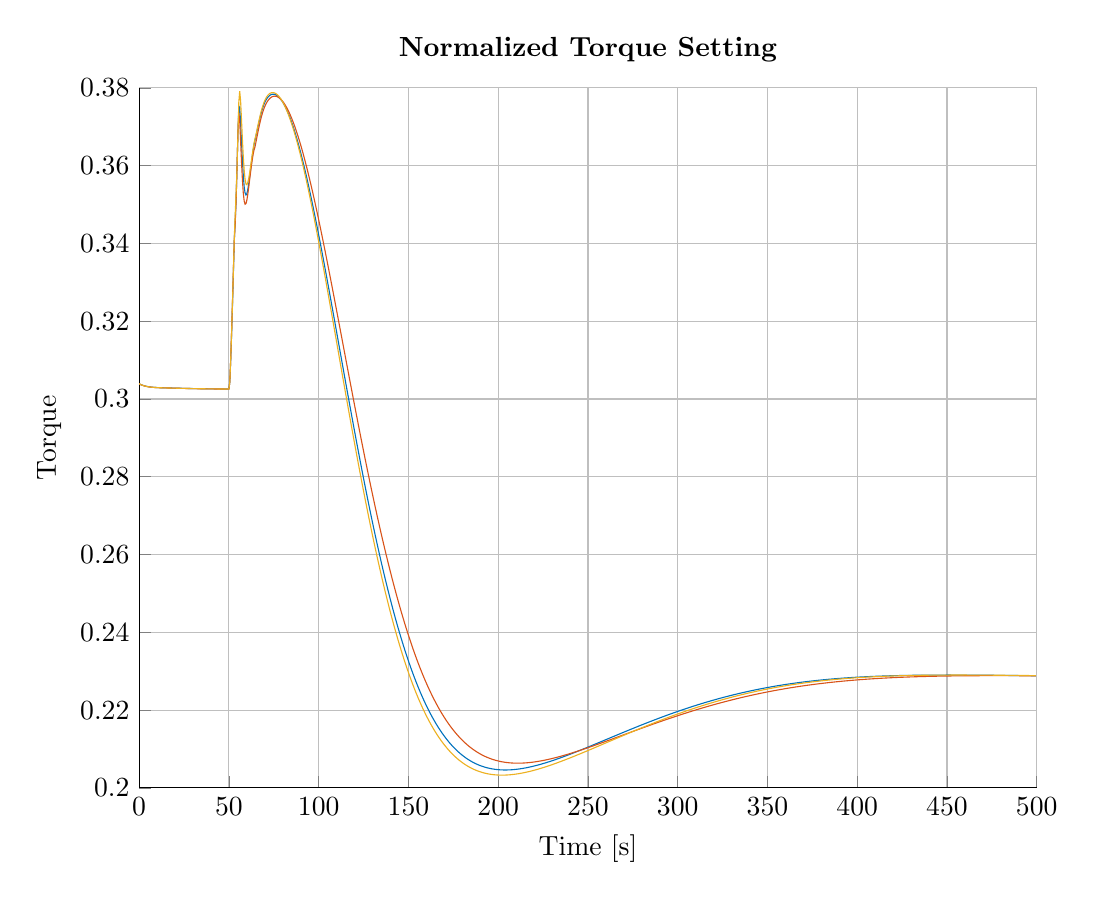
\begin{tikzpicture}

\begin{axis}[%
width=4.488in,
height=3.5in,
at={(0.791in,0.547in)},
scale only axis,
xmin=0,
xmax=500,
xlabel={Time [s]},
xmajorgrids,
ymin=0.2,
ymax=0.38,
ylabel={Torque},
ymajorgrids,
axis background/.style={fill=white},
title style={font=\bfseries},
title={Normalized Torque Setting},
axis x line*=bottom,
axis y line*=left
]
\addplot [color=mycolor1,solid,forget plot]
  table[row sep=crcr]{%
0	0.3039573152\\
0.5	0.303775988\\
1	0.303680777\\
1.5	0.303591625\\
2	0.303511058\\
2.5	0.303437863\\
3	0.303371714\\
3.5	0.303312209\\
4	0.303258903\\
4.5	0.30321133\\
5	0.303169016\\
5.5	0.303131484\\
6	0.30309827\\
6.5	0.303068925\\
7	0.303043022\\
7.5	0.30302016\\
8	0.30299996\\
8.5	0.30298209\\
9	0.30296622\\
9.5	0.30295207\\
10	0.30293939\\
10.5	0.30292794\\
11	0.30291752\\
11.5	0.30290797\\
12	0.30289911\\
12.5	0.30289083\\
13	0.302883\\
13.5	0.30287554\\
14	0.30286837\\
14.5	0.30286141\\
15	0.30285462\\
15.5	0.30284795\\
16	0.30284137\\
16.5	0.30283486\\
17	0.3028284\\
17.5	0.30282197\\
18	0.30281558\\
18.5	0.30280921\\
19	0.30280286\\
19.5	0.30279654\\
20	0.30279025\\
20.5	0.302784\\
21	0.30277779\\
21.5	0.30277162\\
22	0.30276551\\
22.5	0.30275946\\
23	0.30275348\\
23.5	0.30274757\\
24	0.30274173\\
24.5	0.30273598\\
25	0.30273032\\
25.5	0.30272476\\
26	0.30271928\\
26.5	0.30271391\\
27	0.30270864\\
27.5	0.30270347\\
28	0.30269841\\
28.5	0.30269345\\
29	0.3026886\\
29.5	0.30268385\\
30	0.30267921\\
30.5	0.30267467\\
31	0.30267023\\
31.5	0.3026659\\
32	0.30266167\\
32.5	0.30265754\\
33	0.30265351\\
33.5	0.30264957\\
34	0.30264573\\
34.5	0.30264198\\
35	0.30263832\\
35.5	0.30263475\\
36	0.30263126\\
36.5	0.30262786\\
37	0.30262454\\
37.5	0.3026213\\
38	0.30261814\\
38.5	0.30261505\\
39	0.30261204\\
39.5	0.3026091\\
40	0.30260623\\
40.5	0.30260343\\
41	0.30260069\\
41.5	0.30259802\\
42	0.30259541\\
42.5	0.30259287\\
43	0.30259038\\
43.5	0.30258795\\
44	0.30258558\\
44.5	0.30258327\\
45	0.30258101\\
45.5	0.3025788\\
46	0.30257665\\
46.5	0.30257454\\
47	0.30257249\\
47.5	0.30257048\\
48	0.30256852\\
48.5	0.3025666\\
49	0.30256473\\
49.5	0.30256291\\
50	0.30256112\\
50.5	0.304394478\\
51	0.31005118\\
51.5	0.3167577\\
52	0.3244155\\
52.5	0.332599\\
53	0.3409423\\
53.5	0.3457664\\
54	0.3514671\\
54.5	0.3592328\\
55	0.3680617\\
55.5	0.3746969\\
56	0.3750856\\
56.5	0.371095\\
57	0.3662848\\
57.5	0.3615689\\
58	0.3575059\\
58.5	0.3545839\\
59	0.3529578\\
59.5	0.3524559\\
60	0.3528279\\
60.5	0.3538361\\
61	0.3552738\\
61.5	0.356968\\
62	0.358779\\
62.5	0.360597\\
63	0.3623409\\
63.5	0.3639582\\
64	0.3654233\\
64.5	0.3665418\\
65	0.3674821\\
65.5	0.3685874\\
66	0.3696727\\
66.5	0.3707071\\
67	0.3717085\\
67.5	0.3726746\\
68	0.3735685\\
68.5	0.374377\\
69	0.3750961\\
69.5	0.3757275\\
70	0.3762754\\
70.5	0.3767459\\
71	0.3771453\\
71.5	0.3774796\\
72	0.3777542\\
72.5	0.3779738\\
73	0.3781422\\
73.5	0.3782629\\
74	0.3783385\\
74.5	0.3783715\\
75	0.3783635\\
75.5	0.3783164\\
76	0.3782313\\
76.5	0.3781093\\
77	0.3779515\\
77.5	0.3777586\\
78	0.3775314\\
78.5	0.3772706\\
79	0.3769767\\
79.5	0.3766505\\
80	0.3762924\\
80.5	0.3759031\\
81	0.375483\\
81.5	0.3750327\\
82	0.3745528\\
82.5	0.3740438\\
83	0.3735062\\
83.5	0.3729406\\
84	0.3723476\\
84.5	0.3717277\\
85	0.3710814\\
85.5	0.3704093\\
86	0.3697121\\
86.5	0.3689901\\
87	0.3682441\\
87.5	0.3674746\\
88	0.366682\\
88.5	0.3658671\\
89	0.3650303\\
89.5	0.3641722\\
90	0.3632934\\
90.5	0.3623945\\
91	0.3614759\\
91.5	0.3605382\\
92	0.3595821\\
92.5	0.358608\\
93	0.3576164\\
93.5	0.356608\\
94	0.3555833\\
94.5	0.3545428\\
95	0.3534869\\
95.5	0.3524164\\
96	0.3513316\\
96.5	0.3502332\\
97	0.3491215\\
97.5	0.3479972\\
98	0.3468608\\
98.5	0.3457127\\
99	0.3445534\\
99.5	0.3433835\\
100	0.3422035\\
100.5	0.3410137\\
101	0.3398148\\
101.5	0.3386072\\
102	0.3373913\\
102.5	0.3361676\\
103	0.3349366\\
103.5	0.3336988\\
104	0.3324546\\
104.5	0.3312044\\
105	0.3299487\\
105.5	0.3286879\\
106	0.3274225\\
106.5	0.3261529\\
107	0.3248794\\
107.5	0.3236026\\
108	0.3223228\\
108.5	0.3210404\\
109	0.3197558\\
109.5	0.3184695\\
110	0.3171818\\
110.5	0.315893\\
111	0.3146036\\
111.5	0.31331389\\
112	0.31202429\\
112.5	0.31073512\\
113	0.30944674\\
113.5	0.30815949\\
114	0.30687372\\
114.5	0.30558974\\
115	0.304307896\\
115.5	0.303028495\\
116	0.30175185\\
116.5	0.30047828\\
117	0.29920807\\
117.5	0.29794152\\
118	0.29667892\\
118.5	0.29542055\\
119	0.29416668\\
119.5	0.2929176\\
120	0.2916735\\
120.5	0.2904348\\
121	0.2892016\\
121.5	0.2879742\\
122	0.2867528\\
122.5	0.2855377\\
123	0.284329\\
123.5	0.2831271\\
124	0.2819321\\
124.5	0.2807442\\
125	0.2795636\\
125.5	0.2783906\\
126	0.2772252\\
126.5	0.2760678\\
127	0.2749184\\
127.5	0.2737773\\
128	0.2726445\\
128.5	0.2715204\\
129	0.2704049\\
129.5	0.2692983\\
130	0.2682008\\
130.5	0.2671123\\
131	0.2660331\\
131.5	0.2649633\\
132	0.2639031\\
132.5	0.2628524\\
133	0.2618115\\
133.5	0.2607804\\
134	0.2597593\\
134.5	0.2587481\\
135	0.2577471\\
135.5	0.2567562\\
136	0.2557756\\
136.5	0.2548054\\
137	0.2538455\\
137.5	0.2528961\\
138	0.2519572\\
138.5	0.2510288\\
139	0.2501111\\
139.5	0.249204\\
140	0.2483075\\
140.5	0.2474218\\
141	0.2465469\\
141.5	0.2456826\\
142	0.2448292\\
142.5	0.2439866\\
143	0.2431547\\
143.5	0.2423337\\
144	0.2415235\\
144.5	0.2407241\\
145	0.2399355\\
145.5	0.2391576\\
146	0.2383906\\
146.5	0.2376343\\
147	0.2368888\\
147.5	0.236154\\
148	0.2354298\\
148.5	0.2347164\\
149	0.2340135\\
149.5	0.2333212\\
150	0.2326395\\
150.5	0.2319683\\
151	0.2313076\\
151.5	0.2306572\\
152	0.2300172\\
152.5	0.2293876\\
153	0.2287682\\
153.5	0.2281589\\
154	0.2275598\\
154.5	0.2269708\\
155	0.2263918\\
155.5	0.2258227\\
156	0.2252635\\
156.5	0.2247141\\
157	0.2241744\\
157.5	0.2236444\\
158	0.2231239\\
158.5	0.222613\\
159	0.2221114\\
159.5	0.2216193\\
160	0.2211363\\
160.5	0.2206626\\
161	0.2201979\\
161.5	0.2197423\\
162	0.2192955\\
162.5	0.2188577\\
163	0.2184285\\
163.5	0.218008\\
164	0.2175961\\
164.5	0.2171927\\
165	0.2167977\\
165.5	0.2164109\\
166	0.2160324\\
166.5	0.215662\\
167	0.2152996\\
167.5	0.2149451\\
168	0.2145985\\
168.5	0.2142597\\
169	0.2139284\\
169.5	0.2136048\\
170	0.2132886\\
170.5	0.2129798\\
171	0.2126782\\
171.5	0.2123839\\
172	0.2120966\\
172.5	0.2118163\\
173	0.211543\\
173.5	0.2112764\\
174	0.2110166\\
174.5	0.2107634\\
175	0.2105168\\
175.5	0.2102766\\
176	0.2100427\\
176.5	0.2098152\\
177	0.2095938\\
177.5	0.2093784\\
178	0.2091691\\
178.5	0.2089657\\
179	0.2087682\\
179.5	0.2085763\\
180	0.2083902\\
180.5	0.2082095\\
181	0.2080344\\
181.5	0.2078647\\
182	0.2077003\\
182.5	0.2075411\\
183	0.207387\\
183.5	0.2072381\\
184	0.2070941\\
184.5	0.206955\\
185	0.2068208\\
185.5	0.2066913\\
186	0.2065664\\
186.5	0.2064462\\
187	0.2063305\\
187.5	0.2062193\\
188	0.2061124\\
188.5	0.2060098\\
189	0.2059114\\
189.5	0.2058172\\
190	0.2057271\\
190.5	0.205641\\
191	0.2055589\\
191.5	0.2054806\\
192	0.2054062\\
192.5	0.2053354\\
193	0.2052684\\
193.5	0.205205\\
194	0.2051451\\
194.5	0.2050888\\
195	0.2050358\\
195.5	0.2049863\\
196	0.20494\\
196.5	0.204897\\
197	0.2048571\\
197.5	0.2048204\\
198	0.2047868\\
198.5	0.2047562\\
199	0.2047285\\
199.5	0.2047038\\
200	0.2046819\\
200.5	0.2046628\\
201	0.2046464\\
201.5	0.2046328\\
202	0.2046218\\
202.5	0.2046134\\
203	0.2046075\\
203.5	0.2046042\\
204	0.2046033\\
204.5	0.2046048\\
205	0.2046086\\
205.5	0.2046148\\
206	0.2046232\\
206.5	0.2046339\\
207	0.2046467\\
207.5	0.2046617\\
208	0.2046788\\
208.5	0.2046979\\
209	0.204719\\
209.5	0.2047422\\
210	0.2047672\\
210.5	0.2047942\\
211	0.204823\\
211.5	0.2048536\\
212	0.204886\\
212.5	0.2049201\\
213	0.204956\\
213.5	0.2049935\\
214	0.2050327\\
214.5	0.2050735\\
215	0.2051159\\
215.5	0.2051598\\
216	0.2052052\\
216.5	0.2052521\\
217	0.2053004\\
217.5	0.2053502\\
218	0.2054013\\
218.5	0.2054538\\
219	0.2055076\\
219.5	0.2055627\\
220	0.2056191\\
220.5	0.2056767\\
221	0.2057356\\
221.5	0.2057956\\
222	0.2058568\\
222.5	0.2059191\\
223	0.2059825\\
223.5	0.206047\\
224	0.2061126\\
224.5	0.2061792\\
225	0.2062468\\
225.5	0.2063154\\
226	0.2063849\\
226.5	0.2064554\\
227	0.2065268\\
227.5	0.2065991\\
228	0.2066723\\
228.5	0.2067463\\
229	0.2068212\\
229.5	0.2068969\\
230	0.2069734\\
230.5	0.2070506\\
231	0.2071286\\
231.5	0.2072073\\
232	0.2072867\\
232.5	0.2073669\\
233	0.2074477\\
233.5	0.2075291\\
234	0.2076112\\
234.5	0.2076939\\
235	0.2077773\\
235.5	0.2078612\\
236	0.2079456\\
236.5	0.2080307\\
237	0.2081163\\
237.5	0.2082024\\
238	0.208289\\
238.5	0.2083761\\
239	0.2084636\\
239.5	0.2085517\\
240	0.2086401\\
240.5	0.2087291\\
241	0.2088184\\
241.5	0.2089081\\
242	0.2089982\\
242.5	0.2090888\\
243	0.2091796\\
243.5	0.2092708\\
244	0.2093624\\
244.5	0.2094543\\
245	0.2095465\\
245.5	0.209639\\
246	0.2097317\\
246.5	0.2098248\\
247	0.2099181\\
247.5	0.2100117\\
248	0.2101055\\
248.5	0.2101995\\
249	0.2102938\\
249.5	0.2103883\\
250	0.2104829\\
};
\addplot [color=mycolor1,solid,forget plot]
  table[row sep=crcr]{%
250	0.2104829\\
250.5	0.2105778\\
251	0.2106728\\
251.5	0.210768\\
252	0.2108634\\
252.5	0.2109589\\
253	0.2110545\\
253.5	0.2111503\\
254	0.2112462\\
254.5	0.2113422\\
255	0.2114383\\
255.5	0.2115344\\
256	0.2116307\\
256.5	0.211727\\
257	0.2118234\\
257.5	0.2119199\\
258	0.2120164\\
258.5	0.2121129\\
259	0.2122095\\
259.5	0.2123061\\
260	0.2124027\\
260.5	0.2124993\\
261	0.212596\\
261.5	0.2126926\\
262	0.2127892\\
262.5	0.2128857\\
263	0.2129823\\
263.5	0.2130788\\
264	0.2131752\\
264.5	0.2132716\\
265	0.213368\\
265.5	0.2134643\\
266	0.2135605\\
266.5	0.2136566\\
267	0.2137527\\
267.5	0.2138487\\
268	0.2139445\\
268.5	0.2140403\\
269	0.2141359\\
269.5	0.2142315\\
270	0.2143269\\
270.5	0.2144222\\
271	0.2145174\\
271.5	0.2146124\\
272	0.2147073\\
272.5	0.214802\\
273	0.2148966\\
273.5	0.2149911\\
274	0.2150853\\
274.5	0.2151794\\
275	0.2152734\\
275.5	0.2153671\\
276	0.2154607\\
276.5	0.215554\\
277	0.2156472\\
277.5	0.2157402\\
278	0.215833\\
278.5	0.2159256\\
279	0.2160179\\
279.5	0.2161101\\
280	0.216202\\
280.5	0.2162937\\
281	0.2163852\\
281.5	0.2164765\\
282	0.2165675\\
282.5	0.2166583\\
283	0.2167488\\
283.5	0.2168391\\
284	0.2169291\\
284.5	0.2170189\\
285	0.2171084\\
285.5	0.2171977\\
286	0.2172867\\
286.5	0.2173754\\
287	0.2174639\\
287.5	0.2175521\\
288	0.21764\\
288.5	0.2177276\\
289	0.2178149\\
289.5	0.217902\\
290	0.2179887\\
290.5	0.2180752\\
291	0.2181614\\
291.5	0.2182472\\
292	0.2183328\\
292.5	0.2184181\\
293	0.218503\\
293.5	0.2185877\\
294	0.218672\\
294.5	0.218756\\
295	0.2188397\\
295.5	0.2189231\\
296	0.2190061\\
296.5	0.2190889\\
297	0.2191713\\
297.5	0.2192534\\
298	0.2193351\\
298.5	0.2194165\\
299	0.2194976\\
299.5	0.2195783\\
300	0.2196587\\
300.5	0.2197387\\
301	0.2198184\\
301.5	0.2198978\\
302	0.2199768\\
302.5	0.2200555\\
303	0.2201338\\
303.5	0.2202117\\
304	0.2202893\\
304.5	0.2203666\\
305	0.2204435\\
305.5	0.22052\\
306	0.2205962\\
306.5	0.220672\\
307	0.2207474\\
307.5	0.2208225\\
308	0.2208972\\
308.5	0.2209715\\
309	0.2210455\\
309.5	0.2211191\\
310	0.2211923\\
310.5	0.2212652\\
311	0.2213377\\
311.5	0.2214098\\
312	0.2214815\\
312.5	0.2215529\\
313	0.2216238\\
313.5	0.2216944\\
314	0.2217647\\
314.5	0.2218345\\
315	0.221904\\
315.5	0.221973\\
316	0.2220417\\
316.5	0.22211\\
317	0.222178\\
317.5	0.2222455\\
318	0.2223127\\
318.5	0.2223794\\
319	0.2224458\\
319.5	0.2225118\\
320	0.2225774\\
320.5	0.2226426\\
321	0.2227075\\
321.5	0.2227719\\
322	0.222836\\
322.5	0.2228996\\
323	0.2229629\\
323.5	0.2230258\\
324	0.2230883\\
324.5	0.2231504\\
325	0.2232121\\
325.5	0.2232735\\
326	0.2233344\\
326.5	0.2233949\\
327	0.2234551\\
327.5	0.2235149\\
328	0.2235742\\
328.5	0.2236332\\
329	0.2236918\\
329.5	0.22375\\
330	0.2238078\\
330.5	0.2238653\\
331	0.2239223\\
331.5	0.2239789\\
332	0.2240352\\
332.5	0.2240911\\
333	0.2241465\\
333.5	0.2242016\\
334	0.2242563\\
334.5	0.2243106\\
335	0.2243646\\
335.5	0.2244181\\
336	0.2244713\\
336.5	0.224524\\
337	0.2245764\\
337.5	0.2246284\\
338	0.22468\\
338.5	0.2247313\\
339	0.2247821\\
339.5	0.2248326\\
340	0.2248827\\
340.5	0.2249324\\
341	0.2249817\\
341.5	0.2250306\\
342	0.2250792\\
342.5	0.2251274\\
343	0.2251752\\
343.5	0.2252226\\
344	0.2252697\\
344.5	0.2253164\\
345	0.2253627\\
345.5	0.2254086\\
346	0.2254542\\
346.5	0.2254993\\
347	0.2255442\\
347.5	0.2255886\\
348	0.2256327\\
348.5	0.2256764\\
349	0.2257198\\
349.5	0.2257627\\
350	0.2258053\\
350.5	0.2258476\\
351	0.2258895\\
351.5	0.225931\\
352	0.2259722\\
352.5	0.226013\\
353	0.2260534\\
353.5	0.2260935\\
354	0.2261333\\
354.5	0.2261727\\
355	0.2262117\\
355.5	0.2262504\\
356	0.2262887\\
356.5	0.2263267\\
357	0.2263643\\
357.5	0.2264016\\
358	0.2264385\\
358.5	0.2264751\\
359	0.2265114\\
359.5	0.2265473\\
360	0.2265828\\
360.5	0.2266181\\
361	0.2266529\\
361.5	0.2266875\\
362	0.2267217\\
362.5	0.2267556\\
363	0.2267892\\
363.5	0.2268224\\
364	0.2268553\\
364.5	0.2268878\\
365	0.2269201\\
365.5	0.226952\\
366	0.2269836\\
366.5	0.2270148\\
367	0.2270458\\
367.5	0.2270764\\
368	0.2271067\\
368.5	0.2271367\\
369	0.2271664\\
369.5	0.2271958\\
370	0.2272248\\
370.5	0.2272536\\
371	0.227282\\
371.5	0.2273101\\
372	0.2273379\\
372.5	0.2273655\\
373	0.2273927\\
373.5	0.2274196\\
374	0.2274462\\
374.5	0.2274726\\
375	0.2274986\\
375.5	0.2275243\\
376	0.2275498\\
376.5	0.2275749\\
377	0.2275998\\
377.5	0.2276244\\
378	0.2276486\\
378.5	0.2276726\\
379	0.2276964\\
379.5	0.2277198\\
380	0.227743\\
380.5	0.2277659\\
381	0.2277885\\
381.5	0.2278108\\
382	0.2278329\\
382.5	0.2278547\\
383	0.2278762\\
383.5	0.2278975\\
384	0.2279185\\
384.5	0.2279392\\
385	0.2279597\\
385.5	0.2279799\\
386	0.2279998\\
386.5	0.2280195\\
387	0.2280389\\
387.5	0.2280581\\
388	0.2280771\\
388.5	0.2280957\\
389	0.2281142\\
389.5	0.2281324\\
390	0.2281503\\
390.5	0.228168\\
391	0.2281855\\
391.5	0.2282027\\
392	0.2282197\\
392.5	0.2282364\\
393	0.2282529\\
393.5	0.2282692\\
394	0.2282852\\
394.5	0.2283011\\
395	0.2283166\\
395.5	0.228332\\
396	0.2283471\\
396.5	0.2283621\\
397	0.2283768\\
397.5	0.2283912\\
398	0.2284055\\
398.5	0.2284195\\
399	0.2284334\\
399.5	0.228447\\
400	0.2284604\\
400.5	0.2284736\\
401	0.2284866\\
401.5	0.2284994\\
402	0.228512\\
402.5	0.2285243\\
403	0.2285365\\
403.5	0.2285485\\
404	0.2285603\\
404.5	0.2285719\\
405	0.2285833\\
405.5	0.2285945\\
406	0.2286055\\
406.5	0.2286163\\
407	0.228627\\
407.5	0.2286374\\
408	0.2286477\\
408.5	0.2286578\\
409	0.2286677\\
409.5	0.2286774\\
410	0.228687\\
410.5	0.2286963\\
411	0.2287055\\
411.5	0.2287146\\
412	0.2287234\\
412.5	0.2287321\\
413	0.2287407\\
413.5	0.228749\\
414	0.2287572\\
414.5	0.2287652\\
415	0.2287731\\
415.5	0.2287808\\
416	0.2287884\\
416.5	0.2287958\\
417	0.228803\\
417.5	0.2288101\\
418	0.228817\\
418.5	0.2288238\\
419	0.2288305\\
419.5	0.228837\\
420	0.2288433\\
420.5	0.2288495\\
421	0.2288556\\
421.5	0.2288615\\
422	0.2288673\\
422.5	0.2288729\\
423	0.2288784\\
423.5	0.2288838\\
424	0.228889\\
424.5	0.2288941\\
425	0.2288991\\
425.5	0.228904\\
426	0.2289087\\
426.5	0.2289133\\
427	0.2289177\\
427.5	0.2289221\\
428	0.2289263\\
428.5	0.2289304\\
429	0.2289344\\
429.5	0.2289382\\
430	0.228942\\
430.5	0.2289456\\
431	0.2289491\\
431.5	0.2289525\\
432	0.2289558\\
432.5	0.228959\\
433	0.2289621\\
433.5	0.2289651\\
434	0.2289679\\
434.5	0.2289707\\
435	0.2289733\\
435.5	0.2289759\\
436	0.2289783\\
436.5	0.2289807\\
437	0.228983\\
437.5	0.2289851\\
438	0.2289872\\
438.5	0.2289892\\
439	0.228991\\
439.5	0.2289928\\
440	0.2289945\\
440.5	0.2289961\\
441	0.2289976\\
441.5	0.2289991\\
442	0.2290004\\
442.5	0.2290017\\
443	0.2290029\\
443.5	0.2290039\\
444	0.229005\\
444.5	0.2290059\\
445	0.2290068\\
445.5	0.2290075\\
446	0.2290082\\
446.5	0.2290089\\
447	0.2290094\\
447.5	0.2290099\\
448	0.2290103\\
448.5	0.2290106\\
449	0.2290109\\
449.5	0.2290111\\
450	0.2290112\\
450.5	0.2290113\\
451	0.2290113\\
451.5	0.2290112\\
452	0.2290111\\
452.5	0.2290109\\
453	0.2290106\\
453.5	0.2290103\\
454	0.22901\\
454.5	0.2290095\\
455	0.229009\\
455.5	0.2290085\\
456	0.2290079\\
456.5	0.2290072\\
457	0.2290065\\
457.5	0.2290057\\
458	0.2290049\\
458.5	0.2290041\\
459	0.2290031\\
459.5	0.2290022\\
460	0.2290012\\
460.5	0.2290001\\
461	0.228999\\
461.5	0.2289978\\
462	0.2289966\\
462.5	0.2289954\\
463	0.2289941\\
463.5	0.2289928\\
464	0.2289914\\
464.5	0.22899\\
465	0.2289885\\
465.5	0.2289871\\
466	0.2289855\\
466.5	0.228984\\
467	0.2289824\\
467.5	0.2289807\\
468	0.228979\\
468.5	0.2289773\\
469	0.2289756\\
469.5	0.2289738\\
470	0.228972\\
470.5	0.2289702\\
471	0.2289683\\
471.5	0.2289664\\
472	0.2289645\\
472.5	0.2289625\\
473	0.2289605\\
473.5	0.2289585\\
474	0.2289565\\
474.5	0.2289544\\
475	0.2289523\\
475.5	0.2289502\\
476	0.2289481\\
476.5	0.2289459\\
477	0.2289437\\
477.5	0.2289415\\
478	0.2289393\\
478.5	0.2289371\\
479	0.2289348\\
479.5	0.2289325\\
480	0.2289302\\
480.5	0.2289279\\
481	0.2289255\\
481.5	0.2289232\\
482	0.2289208\\
482.5	0.2289184\\
483	0.228916\\
483.5	0.2289136\\
484	0.2289111\\
484.5	0.2289087\\
485	0.2289062\\
485.5	0.2289038\\
486	0.2289013\\
486.5	0.2288988\\
487	0.2288962\\
487.5	0.2288937\\
488	0.2288912\\
488.5	0.2288886\\
489	0.2288861\\
489.5	0.2288835\\
490	0.228881\\
490.5	0.2288784\\
491	0.2288758\\
491.5	0.2288732\\
492	0.2288706\\
492.5	0.228868\\
493	0.2288654\\
493.5	0.2288628\\
494	0.2288601\\
494.5	0.2288575\\
495	0.2288549\\
495.5	0.2288522\\
496	0.2288496\\
496.5	0.2288469\\
497	0.2288443\\
497.5	0.2288416\\
498	0.228839\\
498.5	0.2288363\\
499	0.2288337\\
499.5	0.228831\\
};
\addplot [color=mycolor2,solid,forget plot]
  table[row sep=crcr]{%
0	0.3039552245\\
0.5	0.303765592\\
1	0.303666922\\
1.5	0.303574787\\
2	0.30349186\\
2.5	0.30341683\\
3	0.303349327\\
3.5	0.303288902\\
4	0.303235058\\
4.5	0.303187277\\
5	0.303145034\\
5.5	0.303107805\\
6	0.303075079\\
6.5	0.303046365\\
7	0.303021198\\
7.5	0.30299914\\
8	0.30297979\\
8.5	0.30296278\\
9	0.30294777\\
9.5	0.30293446\\
10	0.30292257\\
10.5	0.30291187\\
11	0.30290214\\
11.5	0.30289321\\
12	0.30288491\\
12.5	0.30287712\\
13	0.30286972\\
13.5	0.30286262\\
14	0.30285574\\
14.5	0.30284902\\
15	0.30284241\\
15.5	0.30283587\\
16	0.30282937\\
16.5	0.3028229\\
17	0.30281644\\
17.5	0.30280998\\
18	0.30280353\\
18.5	0.30279707\\
19	0.30279063\\
19.5	0.30278419\\
20	0.30277777\\
20.5	0.30277137\\
21	0.30276501\\
21.5	0.30275869\\
22	0.30275243\\
22.5	0.30274622\\
23	0.30274008\\
23.5	0.30273401\\
24	0.30272803\\
24.5	0.30272213\\
25	0.30271633\\
25.5	0.30271062\\
26	0.30270501\\
26.5	0.30269951\\
27	0.30269412\\
27.5	0.30268883\\
28	0.30268365\\
28.5	0.30267859\\
29	0.30267363\\
29.5	0.30266878\\
30	0.30266404\\
30.5	0.30265942\\
31	0.30265489\\
31.5	0.30265048\\
32	0.30264617\\
32.5	0.30264196\\
33	0.30263785\\
33.5	0.30263384\\
34	0.30262992\\
34.5	0.3026261\\
35	0.30262237\\
35.5	0.30261874\\
36	0.30261518\\
36.5	0.30261172\\
37	0.30260833\\
37.5	0.30260503\\
38	0.30260181\\
38.5	0.30259866\\
39	0.30259559\\
39.5	0.30259259\\
40	0.30258966\\
40.5	0.3025868\\
41	0.30258401\\
41.5	0.30258128\\
42	0.30257862\\
42.5	0.30257601\\
43	0.30257347\\
43.5	0.30257099\\
44	0.30256857\\
44.5	0.3025662\\
45	0.30256389\\
45.5	0.30256163\\
46	0.30255943\\
46.5	0.30255727\\
47	0.30255516\\
47.5	0.30255311\\
48	0.3025511\\
48.5	0.30254913\\
49	0.30254722\\
49.5	0.30254534\\
50	0.30254351\\
50.5	0.304471449\\
51	0.31042517\\
51.5	0.3174263\\
52	0.325291\\
52.5	0.3334964\\
53	0.3408456\\
53.5	0.3451152\\
54	0.3508922\\
54.5	0.3592195\\
55	0.3683954\\
55.5	0.3736534\\
56	0.3715522\\
56.5	0.3663626\\
57	0.3610624\\
57.5	0.356449\\
58	0.3529859\\
58.5	0.3509046\\
59	0.3500809\\
59.5	0.3502514\\
60	0.3511626\\
60.5	0.3525872\\
61	0.3543252\\
61.5	0.3562077\\
62	0.3580983\\
62.5	0.3598939\\
63	0.3615241\\
63.5	0.3629525\\
64	0.3640551\\
64.5	0.3647738\\
65	0.3659146\\
65.5	0.3671063\\
66	0.3682674\\
66.5	0.3693898\\
67	0.3704737\\
67.5	0.3714837\\
68	0.3724073\\
68.5	0.3732412\\
69	0.3739872\\
69.5	0.3746488\\
70	0.3752313\\
70.5	0.375741\\
71	0.3761835\\
71.5	0.3765645\\
72	0.3768889\\
72.5	0.3771609\\
73	0.3773843\\
73.5	0.3775621\\
74	0.3776969\\
74.5	0.3777909\\
75	0.3778458\\
75.5	0.3778632\\
76	0.3778442\\
76.5	0.37779\\
77	0.3777015\\
77.5	0.3775793\\
78	0.3774244\\
78.5	0.3772372\\
79	0.3770184\\
79.5	0.3767686\\
80	0.3764883\\
80.5	0.376178\\
81	0.3758383\\
81.5	0.3754696\\
82	0.3750724\\
82.5	0.3746474\\
83	0.3741949\\
83.5	0.3737155\\
84	0.3732096\\
84.5	0.3726779\\
85	0.3721207\\
85.5	0.3715386\\
86	0.3709322\\
86.5	0.3703018\\
87	0.3696481\\
87.5	0.3689715\\
88	0.3682725\\
88.5	0.3675517\\
89	0.3668096\\
89.5	0.3660466\\
90	0.3652632\\
90.5	0.36446\\
91	0.3636375\\
91.5	0.3627962\\
92	0.3619365\\
92.5	0.361059\\
93	0.3601641\\
93.5	0.3592523\\
94	0.3583242\\
94.5	0.3573802\\
95	0.3564208\\
95.5	0.3554464\\
96	0.3544576\\
96.5	0.3534548\\
97	0.3524385\\
97.5	0.3514092\\
98	0.3503673\\
98.5	0.3493133\\
99	0.3482476\\
99.5	0.3471707\\
100	0.346083\\
100.5	0.344985\\
101	0.3438772\\
101.5	0.3427599\\
102	0.3416336\\
102.5	0.3404987\\
103	0.3393557\\
103.5	0.3382049\\
104	0.3370469\\
104.5	0.3358819\\
105	0.3347104\\
105.5	0.3335328\\
106	0.3323496\\
106.5	0.331161\\
107	0.3299675\\
107.5	0.3287695\\
108	0.3275673\\
108.5	0.3263614\\
109	0.325152\\
109.5	0.3239397\\
110	0.3227246\\
110.5	0.3215072\\
111	0.3202879\\
111.5	0.3190669\\
112	0.3178446\\
112.5	0.3166214\\
113	0.3153975\\
113.5	0.3141734\\
114	0.31294924\\
114.5	0.31172545\\
115	0.31050231\\
115.5	0.30928011\\
116	0.30805916\\
116.5	0.30683976\\
117	0.30562219\\
117.5	0.304406727\\
118	0.30319366\\
118.5	0.30198326\\
119	0.30077579\\
119.5	0.29957151\\
120	0.29837068\\
120.5	0.29717356\\
121	0.29598038\\
121.5	0.29479139\\
122	0.2936068\\
122.5	0.2924269\\
123	0.2912519\\
123.5	0.2900819\\
124	0.2889173\\
124.5	0.2877582\\
125	0.2866048\\
125.5	0.2854573\\
126	0.284316\\
126.5	0.2831809\\
127	0.2820524\\
127.5	0.2809304\\
128	0.2798154\\
128.5	0.2787073\\
129	0.2776064\\
129.5	0.2765128\\
130	0.2754266\\
130.5	0.2743481\\
131	0.2732773\\
131.5	0.2722144\\
132	0.2711596\\
132.5	0.2701129\\
133	0.2690744\\
133.5	0.2680443\\
134	0.2670228\\
134.5	0.2660098\\
135	0.2650055\\
135.5	0.2640101\\
136	0.2630235\\
136.5	0.2620459\\
137	0.2610774\\
137.5	0.260118\\
138	0.2591678\\
138.5	0.258227\\
139	0.2572954\\
139.5	0.2563733\\
140	0.2554607\\
140.5	0.2545575\\
141	0.253664\\
141.5	0.25278\\
142	0.2519057\\
142.5	0.2510411\\
143	0.2501863\\
143.5	0.2493411\\
144	0.2485058\\
144.5	0.2476802\\
145	0.2468645\\
145.5	0.2460586\\
146	0.2452625\\
146.5	0.2444762\\
147	0.2436998\\
147.5	0.2429333\\
148	0.2421766\\
148.5	0.2414297\\
149	0.2406926\\
149.5	0.2399654\\
150	0.239248\\
150.5	0.2385403\\
151	0.2378424\\
151.5	0.2371542\\
152	0.2364757\\
152.5	0.2358069\\
153	0.2351477\\
153.5	0.2344981\\
154	0.2338581\\
154.5	0.2332276\\
155	0.2326066\\
155.5	0.2319951\\
156	0.2313929\\
156.5	0.2308001\\
157	0.2302165\\
157.5	0.2296422\\
158	0.2290771\\
158.5	0.2285211\\
159	0.2279742\\
159.5	0.2274363\\
160	0.2269074\\
160.5	0.2263873\\
161	0.2258761\\
161.5	0.2253736\\
162	0.2248798\\
162.5	0.2243947\\
163	0.223918\\
163.5	0.2234499\\
164	0.2229902\\
164.5	0.2225388\\
165	0.2220956\\
165.5	0.2216607\\
166	0.2212339\\
166.5	0.2208151\\
167	0.2204042\\
167.5	0.2200013\\
168	0.2196061\\
168.5	0.2192187\\
169	0.2188389\\
169.5	0.2184667\\
170	0.218102\\
170.5	0.2177446\\
171	0.2173946\\
171.5	0.2170519\\
172	0.2167162\\
172.5	0.2163877\\
173	0.2160662\\
173.5	0.2157516\\
174	0.2154438\\
174.5	0.2151427\\
175	0.2148484\\
175.5	0.2145606\\
176	0.2142793\\
176.5	0.2140045\\
177	0.213736\\
177.5	0.2134737\\
178	0.2132177\\
178.5	0.2129677\\
179	0.2127237\\
179.5	0.2124857\\
180	0.2122536\\
180.5	0.2120272\\
181	0.2118065\\
181.5	0.2115914\\
182	0.2113819\\
182.5	0.2111779\\
183	0.2109792\\
183.5	0.2107859\\
184	0.2105978\\
184.5	0.2104148\\
185	0.2102369\\
185.5	0.210064\\
186	0.2098961\\
186.5	0.209733\\
187	0.2095748\\
187.5	0.2094212\\
188	0.2092723\\
188.5	0.2091279\\
189	0.2089881\\
189.5	0.2088527\\
190	0.2087216\\
190.5	0.2085949\\
191	0.2084723\\
191.5	0.208354\\
192	0.2082397\\
192.5	0.2081295\\
193	0.2080232\\
193.5	0.2079208\\
194	0.2078223\\
194.5	0.2077275\\
195	0.2076365\\
195.5	0.2075491\\
196	0.2074653\\
196.5	0.207385\\
197	0.2073082\\
197.5	0.2072349\\
198	0.2071648\\
198.5	0.2070981\\
199	0.2070346\\
199.5	0.2069743\\
200	0.2069172\\
200.5	0.2068631\\
201	0.2068121\\
201.5	0.206764\\
202	0.2067188\\
202.5	0.2066766\\
203	0.2066371\\
203.5	0.2066004\\
204	0.2065664\\
204.5	0.2065352\\
205	0.2065065\\
205.5	0.2064804\\
206	0.2064569\\
206.5	0.2064358\\
207	0.2064172\\
207.5	0.2064009\\
208	0.2063871\\
208.5	0.2063755\\
209	0.2063662\\
209.5	0.2063591\\
210	0.2063543\\
210.5	0.2063515\\
211	0.2063509\\
211.5	0.2063523\\
212	0.2063558\\
212.5	0.2063612\\
213	0.2063686\\
213.5	0.2063779\\
214	0.2063891\\
214.5	0.2064022\\
215	0.206417\\
215.5	0.2064336\\
216	0.206452\\
216.5	0.206472\\
217	0.2064937\\
217.5	0.2065171\\
218	0.206542\\
218.5	0.2065686\\
219	0.2065967\\
219.5	0.2066263\\
220	0.2066573\\
220.5	0.2066898\\
221	0.2067238\\
221.5	0.2067591\\
222	0.2067958\\
222.5	0.2068339\\
223	0.2068732\\
223.5	0.2069139\\
224	0.2069558\\
224.5	0.2069989\\
225	0.2070432\\
225.5	0.2070887\\
226	0.2071354\\
226.5	0.2071832\\
227	0.2072321\\
227.5	0.2072821\\
228	0.2073331\\
228.5	0.2073852\\
229	0.2074383\\
229.5	0.2074924\\
230	0.2075474\\
230.5	0.2076034\\
231	0.2076603\\
231.5	0.2077182\\
232	0.2077769\\
232.5	0.2078365\\
233	0.2078969\\
233.5	0.2079582\\
234	0.2080202\\
234.5	0.2080831\\
235	0.2081467\\
235.5	0.2082111\\
236	0.2082762\\
236.5	0.208342\\
237	0.2084085\\
237.5	0.2084757\\
238	0.2085435\\
238.5	0.2086121\\
239	0.2086812\\
239.5	0.2087509\\
240	0.2088213\\
240.5	0.2088922\\
241	0.2089637\\
241.5	0.2090358\\
242	0.2091084\\
242.5	0.2091815\\
243	0.2092552\\
243.5	0.2093293\\
244	0.2094039\\
244.5	0.209479\\
245	0.2095545\\
245.5	0.2096305\\
246	0.2097069\\
246.5	0.2097837\\
247	0.2098609\\
247.5	0.2099385\\
248	0.2100165\\
248.5	0.2100948\\
249	0.2101735\\
249.5	0.2102526\\
250	0.210332\\
};
\addplot [color=mycolor2,solid,forget plot]
  table[row sep=crcr]{%
250	0.210332\\
250.5	0.2104117\\
251	0.2104917\\
251.5	0.210572\\
252	0.2106526\\
252.5	0.2107334\\
253	0.2108146\\
253.5	0.2108959\\
254	0.2109776\\
254.5	0.2110594\\
255	0.2111415\\
255.5	0.2112238\\
256	0.2113064\\
256.5	0.2113891\\
257	0.211472\\
257.5	0.211555\\
258	0.2116383\\
258.5	0.2117217\\
259	0.2118053\\
259.5	0.211889\\
260	0.2119728\\
260.5	0.2120568\\
261	0.2121408\\
261.5	0.212225\\
262	0.2123093\\
262.5	0.2123937\\
263	0.2124782\\
263.5	0.2125628\\
264	0.2126474\\
264.5	0.2127321\\
265	0.2128168\\
265.5	0.2129016\\
266	0.2129865\\
266.5	0.2130714\\
267	0.2131563\\
267.5	0.2132412\\
268	0.2133262\\
268.5	0.2134111\\
269	0.2134961\\
269.5	0.2135811\\
270	0.213666\\
270.5	0.213751\\
271	0.2138359\\
271.5	0.2139208\\
272	0.2140056\\
272.5	0.2140904\\
273	0.2141752\\
273.5	0.2142599\\
274	0.2143446\\
274.5	0.2144292\\
275	0.2145138\\
275.5	0.2145983\\
276	0.2146826\\
276.5	0.214767\\
277	0.2148512\\
277.5	0.2149353\\
278	0.2150194\\
278.5	0.2151033\\
279	0.2151872\\
279.5	0.2152709\\
280	0.2153545\\
280.5	0.215438\\
281	0.2155214\\
281.5	0.2156046\\
282	0.2156877\\
282.5	0.2157707\\
283	0.2158535\\
283.5	0.2159362\\
284	0.2160187\\
284.5	0.2161011\\
285	0.2161834\\
285.5	0.2162654\\
286	0.2163473\\
286.5	0.2164291\\
287	0.2165106\\
287.5	0.216592\\
288	0.2166732\\
288.5	0.2167543\\
289	0.2168351\\
289.5	0.2169158\\
290	0.2169962\\
290.5	0.2170765\\
291	0.2171566\\
291.5	0.2172364\\
292	0.2173161\\
292.5	0.2173955\\
293	0.2174748\\
293.5	0.2175538\\
294	0.2176326\\
294.5	0.2177112\\
295	0.2177896\\
295.5	0.2178677\\
296	0.2179456\\
296.5	0.2180233\\
297	0.2181008\\
297.5	0.218178\\
298	0.218255\\
298.5	0.2183317\\
299	0.2184082\\
299.5	0.2184845\\
300	0.2185605\\
300.5	0.2186362\\
301	0.2187117\\
301.5	0.218787\\
302	0.218862\\
302.5	0.2189367\\
303	0.2190112\\
303.5	0.2190854\\
304	0.2191593\\
304.5	0.219233\\
305	0.2193064\\
305.5	0.2193795\\
306	0.2194524\\
306.5	0.219525\\
307	0.2195973\\
307.5	0.2196693\\
308	0.2197411\\
308.5	0.2198126\\
309	0.2198838\\
309.5	0.2199547\\
310	0.2200253\\
310.5	0.2200956\\
311	0.2201657\\
311.5	0.2202354\\
312	0.2203049\\
312.5	0.2203741\\
313	0.220443\\
313.5	0.2205115\\
314	0.2205798\\
314.5	0.2206478\\
315	0.2207155\\
315.5	0.2207829\\
316	0.22085\\
316.5	0.2209168\\
317	0.2209833\\
317.5	0.2210494\\
318	0.2211153\\
318.5	0.2211809\\
319	0.2212461\\
319.5	0.2213111\\
320	0.2213757\\
320.5	0.2214401\\
321	0.2215041\\
321.5	0.2215678\\
322	0.2216312\\
322.5	0.2216943\\
323	0.221757\\
323.5	0.2218195\\
324	0.2218816\\
324.5	0.2219435\\
325	0.222005\\
325.5	0.2220661\\
326	0.222127\\
326.5	0.2221876\\
327	0.2222478\\
327.5	0.2223077\\
328	0.2223673\\
328.5	0.2224266\\
329	0.2224856\\
329.5	0.2225442\\
330	0.2226025\\
330.5	0.2226605\\
331	0.2227182\\
331.5	0.2227755\\
332	0.2228326\\
332.5	0.2228893\\
333	0.2229457\\
333.5	0.2230017\\
334	0.2230575\\
334.5	0.2231129\\
335	0.223168\\
335.5	0.2232227\\
336	0.2232772\\
336.5	0.2233313\\
337	0.2233851\\
337.5	0.2234386\\
338	0.2234917\\
338.5	0.2235446\\
339	0.2235971\\
339.5	0.2236493\\
340	0.2237011\\
340.5	0.2237527\\
341	0.2238039\\
341.5	0.2238548\\
342	0.2239054\\
342.5	0.2239556\\
343	0.2240056\\
343.5	0.2240552\\
344	0.2241045\\
344.5	0.2241535\\
345	0.2242021\\
345.5	0.2242504\\
346	0.2242984\\
346.5	0.2243461\\
347	0.2243935\\
347.5	0.2244406\\
348	0.2244873\\
348.5	0.2245337\\
349	0.2245798\\
349.5	0.2246256\\
350	0.2246711\\
350.5	0.2247162\\
351	0.2247611\\
351.5	0.2248056\\
352	0.2248498\\
352.5	0.2248937\\
353	0.2249373\\
353.5	0.2249806\\
354	0.2250235\\
354.5	0.2250662\\
355	0.2251085\\
355.5	0.2251506\\
356	0.2251923\\
356.5	0.2252337\\
357	0.2252748\\
357.5	0.2253156\\
358	0.2253561\\
358.5	0.2253963\\
359	0.2254362\\
359.5	0.2254757\\
360	0.225515\\
360.5	0.225554\\
361	0.2255927\\
361.5	0.225631\\
362	0.2256691\\
362.5	0.2257069\\
363	0.2257444\\
363.5	0.2257816\\
364	0.2258184\\
364.5	0.225855\\
365	0.2258913\\
365.5	0.2259273\\
366	0.225963\\
366.5	0.2259985\\
367	0.2260336\\
367.5	0.2260684\\
368	0.226103\\
368.5	0.2261372\\
369	0.2261712\\
369.5	0.2262049\\
370	0.2262383\\
370.5	0.2262714\\
371	0.2263043\\
371.5	0.2263368\\
372	0.2263691\\
372.5	0.2264011\\
373	0.2264328\\
373.5	0.2264643\\
374	0.2264954\\
374.5	0.2265263\\
375	0.226557\\
375.5	0.2265873\\
376	0.2266174\\
376.5	0.2266472\\
377	0.2266767\\
377.5	0.226706\\
378	0.226735\\
378.5	0.2267637\\
379	0.2267922\\
379.5	0.2268204\\
380	0.2268483\\
380.5	0.226876\\
381	0.2269034\\
381.5	0.2269306\\
382	0.2269575\\
382.5	0.2269841\\
383	0.2270105\\
383.5	0.2270367\\
384	0.2270626\\
384.5	0.2270882\\
385	0.2271136\\
385.5	0.2271387\\
386	0.2271636\\
386.5	0.2271882\\
387	0.2272126\\
387.5	0.2272368\\
388	0.2272607\\
388.5	0.2272844\\
389	0.2273078\\
389.5	0.227331\\
390	0.2273539\\
390.5	0.2273766\\
391	0.2273991\\
391.5	0.2274214\\
392	0.2274434\\
392.5	0.2274652\\
393	0.2274867\\
393.5	0.227508\\
394	0.2275291\\
394.5	0.22755\\
395	0.2275706\\
395.5	0.2275911\\
396	0.2276113\\
396.5	0.2276312\\
397	0.227651\\
397.5	0.2276705\\
398	0.2276898\\
398.5	0.227709\\
399	0.2277278\\
399.5	0.2277465\\
400	0.227765\\
400.5	0.2277832\\
401	0.2278013\\
401.5	0.2278191\\
402	0.2278368\\
402.5	0.2278542\\
403	0.2278714\\
403.5	0.2278884\\
404	0.2279053\\
404.5	0.2279219\\
405	0.2279383\\
405.5	0.2279545\\
406	0.2279706\\
406.5	0.2279864\\
407	0.228002\\
407.5	0.2280175\\
408	0.2280328\\
408.5	0.2280478\\
409	0.2280627\\
409.5	0.2280774\\
410	0.2280919\\
410.5	0.2281062\\
411	0.2281204\\
411.5	0.2281343\\
412	0.2281481\\
412.5	0.2281617\\
413	0.2281752\\
413.5	0.2281884\\
414	0.2282015\\
414.5	0.2282144\\
415	0.2282271\\
415.5	0.2282397\\
416	0.2282521\\
416.5	0.2282643\\
417	0.2282763\\
417.5	0.2282882\\
418	0.2282999\\
418.5	0.2283115\\
419	0.2283229\\
419.5	0.2283341\\
420	0.2283452\\
420.5	0.2283561\\
421	0.2283669\\
421.5	0.2283775\\
422	0.228388\\
422.5	0.2283983\\
423	0.2284084\\
423.5	0.2284184\\
424	0.2284282\\
424.5	0.2284379\\
425	0.2284475\\
425.5	0.2284569\\
426	0.2284662\\
426.5	0.2284753\\
427	0.2284843\\
427.5	0.2284931\\
428	0.2285018\\
428.5	0.2285104\\
429	0.2285188\\
429.5	0.2285271\\
430	0.2285352\\
430.5	0.2285433\\
431	0.2285511\\
431.5	0.2285589\\
432	0.2285665\\
432.5	0.228574\\
433	0.2285814\\
433.5	0.2285886\\
434	0.2285958\\
434.5	0.2286027\\
435	0.2286096\\
435.5	0.2286164\\
436	0.228623\\
436.5	0.2286295\\
437	0.2286359\\
437.5	0.2286422\\
438	0.2286483\\
438.5	0.2286544\\
439	0.2286603\\
439.5	0.2286661\\
440	0.2286718\\
440.5	0.2286774\\
441	0.2286829\\
441.5	0.2286883\\
442	0.2286936\\
442.5	0.2286987\\
443	0.2287038\\
443.5	0.2287088\\
444	0.2287136\\
444.5	0.2287184\\
445	0.228723\\
445.5	0.2287276\\
446	0.228732\\
446.5	0.2287364\\
447	0.2287406\\
447.5	0.2287448\\
448	0.2287489\\
448.5	0.2287529\\
449	0.2287567\\
449.5	0.2287605\\
450	0.2287642\\
450.5	0.2287679\\
451	0.2287714\\
451.5	0.2287748\\
452	0.2287782\\
452.5	0.2287814\\
453	0.2287846\\
453.5	0.2287877\\
454	0.2287907\\
454.5	0.2287937\\
455	0.2287965\\
455.5	0.2287993\\
456	0.228802\\
456.5	0.2288046\\
457	0.2288071\\
457.5	0.2288096\\
458	0.228812\\
458.5	0.2288143\\
459	0.2288165\\
459.5	0.2288187\\
460	0.2288208\\
460.5	0.2288228\\
461	0.2288248\\
461.5	0.2288267\\
462	0.2288285\\
462.5	0.2288303\\
463	0.2288319\\
463.5	0.2288336\\
464	0.2288351\\
464.5	0.2288366\\
465	0.228838\\
465.5	0.2288394\\
466	0.2288407\\
466.5	0.228842\\
467	0.2288432\\
467.5	0.2288443\\
468	0.2288453\\
468.5	0.2288464\\
469	0.2288473\\
469.5	0.2288482\\
470	0.2288491\\
470.5	0.2288499\\
471	0.2288506\\
471.5	0.2288513\\
472	0.2288519\\
472.5	0.2288525\\
473	0.228853\\
473.5	0.2288535\\
474	0.2288539\\
474.5	0.2288543\\
475	0.2288546\\
475.5	0.2288549\\
476	0.2288552\\
476.5	0.2288554\\
477	0.2288555\\
477.5	0.2288556\\
478	0.2288557\\
478.5	0.2288557\\
479	0.2288557\\
479.5	0.2288556\\
480	0.2288555\\
480.5	0.2288554\\
481	0.2288552\\
481.5	0.228855\\
482	0.2288547\\
482.5	0.2288544\\
483	0.2288541\\
483.5	0.2288537\\
484	0.2288533\\
484.5	0.2288529\\
485	0.2288524\\
485.5	0.2288519\\
486	0.2288514\\
486.5	0.2288508\\
487	0.2288502\\
487.5	0.2288495\\
488	0.2288489\\
488.5	0.2288482\\
489	0.2288474\\
489.5	0.2288467\\
490	0.2288459\\
490.5	0.2288451\\
491	0.2288442\\
491.5	0.2288433\\
492	0.2288424\\
492.5	0.2288415\\
493	0.2288406\\
493.5	0.2288396\\
494	0.2288386\\
494.5	0.2288376\\
495	0.2288365\\
495.5	0.2288354\\
496	0.2288343\\
496.5	0.2288332\\
497	0.2288321\\
497.5	0.2288309\\
498	0.2288297\\
498.5	0.2288285\\
499	0.2288273\\
499.5	0.2288261\\
};
\addplot [color=mycolor3,solid,forget plot]
  table[row sep=crcr]{%
0	0.3039595053\\
0.5	0.30377925\\
1	0.303678798\\
1.5	0.303585531\\
2	0.303501536\\
2.5	0.303425625\\
3	0.303357386\\
3.5	0.303296341\\
4	0.303241965\\
4.5	0.303193723\\
5	0.303151069\\
5.5	0.303113468\\
6	0.303080398\\
6.5	0.303051362\\
7	0.303025888\\
7.5	0.303003539\\
8	0.30298391\\
8.5	0.30296662\\
9	0.30295135\\
9.5	0.30293779\\
10	0.30292567\\
10.5	0.30291474\\
11	0.30290482\\
11.5	0.3028957\\
12	0.30288724\\
12.5	0.30287931\\
13	0.30287179\\
13.5	0.30286459\\
14	0.30285763\\
14.5	0.30285086\\
15	0.30284422\\
15.5	0.30283767\\
16	0.30283119\\
16.5	0.30282475\\
17	0.30281835\\
17.5	0.30281196\\
18	0.3028056\\
18.5	0.30279925\\
19	0.30279293\\
19.5	0.30278662\\
20	0.30278035\\
20.5	0.30277411\\
21	0.30276791\\
21.5	0.30276177\\
22	0.30275568\\
22.5	0.30274966\\
23	0.30274371\\
23.5	0.30273783\\
24	0.30273204\\
24.5	0.30272634\\
25	0.30272074\\
25.5	0.30271523\\
26	0.30270982\\
26.5	0.30270451\\
27	0.30269931\\
27.5	0.30269422\\
28	0.30268924\\
28.5	0.30268436\\
29	0.30267959\\
29.5	0.30267493\\
30	0.30267038\\
30.5	0.30266593\\
31	0.30266158\\
31.5	0.30265735\\
32	0.30265321\\
32.5	0.30264917\\
33	0.30264523\\
33.5	0.30264138\\
34	0.30263763\\
34.5	0.30263398\\
35	0.30263041\\
35.5	0.30262692\\
36	0.30262353\\
36.5	0.30262021\\
37	0.30261698\\
37.5	0.30261383\\
38	0.30261075\\
38.5	0.30260775\\
39	0.30260482\\
39.5	0.30260196\\
40	0.30259917\\
40.5	0.30259645\\
41	0.3025938\\
41.5	0.3025912\\
42	0.30258867\\
42.5	0.30258621\\
43	0.30258379\\
43.5	0.30258144\\
44	0.30257915\\
44.5	0.3025769\\
45	0.30257472\\
45.5	0.30257258\\
46	0.30257049\\
46.5	0.30256846\\
47	0.30256647\\
47.5	0.30256453\\
48	0.30256264\\
48.5	0.30256079\\
49	0.30255898\\
49.5	0.30255722\\
50	0.3025555\\
50.5	0.304467514\\
51	0.31031926\\
51.5	0.3171748\\
52	0.3249277\\
52.5	0.3331496\\
53	0.3415121\\
53.5	0.3475699\\
54	0.3528995\\
54.5	0.3592749\\
55	0.3677053\\
55.5	0.3762582\\
56	0.3791736\\
56.5	0.3767679\\
57	0.3719053\\
57.5	0.3668808\\
58	0.3623454\\
58.5	0.3587829\\
59	0.3564478\\
59.5	0.3552889\\
60	0.3550915\\
60.5	0.3556223\\
61	0.3566698\\
61.5	0.3580534\\
62	0.3596241\\
62.5	0.3612628\\
63	0.3628772\\
63.5	0.3644008\\
64	0.3657921\\
64.5	0.366835\\
65	0.3677599\\
65.5	0.3688921\\
66	0.3700111\\
66.5	0.3710743\\
67	0.3720974\\
67.5	0.3730826\\
68	0.3739948\\
68.5	0.3748213\\
69	0.3755575\\
69.5	0.3762042\\
70	0.3767645\\
70.5	0.3772437\\
71	0.3776477\\
71.5	0.3779819\\
72	0.3782519\\
72.5	0.3784622\\
73	0.3786173\\
73.5	0.3787207\\
74	0.3787756\\
74.5	0.3787846\\
75	0.3787502\\
75.5	0.3786741\\
76	0.3785582\\
76.5	0.3784036\\
77	0.3782118\\
77.5	0.3779836\\
78	0.37772\\
78.5	0.3774219\\
79	0.3770899\\
79.5	0.3767248\\
80	0.3763272\\
80.5	0.3758976\\
81	0.3754368\\
81.5	0.3749452\\
82	0.3744235\\
82.5	0.3738722\\
83	0.3732919\\
83.5	0.3726831\\
84	0.3720464\\
84.5	0.3713825\\
85	0.3706917\\
85.5	0.3699748\\
86	0.3692324\\
86.5	0.3684649\\
87	0.367673\\
87.5	0.3668573\\
88	0.3660183\\
88.5	0.3651567\\
89	0.364273\\
89.5	0.3633679\\
90	0.3624418\\
90.5	0.3614954\\
91	0.3605293\\
91.5	0.3595441\\
92	0.3585403\\
92.5	0.3575185\\
93	0.3564793\\
93.5	0.3554232\\
94	0.3543508\\
94.5	0.3532627\\
95	0.3521595\\
95.5	0.3510416\\
96	0.3499097\\
96.5	0.3487642\\
97	0.3476058\\
97.5	0.346435\\
98	0.3452523\\
98.5	0.3440582\\
99	0.3428533\\
99.5	0.341638\\
100	0.3404129\\
100.5	0.3391786\\
101	0.3379354\\
101.5	0.3366839\\
102	0.3354247\\
102.5	0.3341581\\
103	0.3328847\\
103.5	0.3316049\\
104	0.3303193\\
104.5	0.3290282\\
105	0.3277321\\
105.5	0.3264316\\
106	0.325127\\
106.5	0.3238187\\
107	0.3225073\\
107.5	0.3211931\\
108	0.3198766\\
108.5	0.3185582\\
109	0.3172382\\
109.5	0.3159172\\
110	0.3145954\\
110.5	0.31327336\\
111	0.31195136\\
111.5	0.31062981\\
112	0.30930907\\
112.5	0.30798951\\
113	0.30667149\\
113.5	0.30535536\\
114	0.3040414711\\
114.5	0.30273015\\
115	0.30142173\\
115.5	0.30011655\\
116	0.2988149\\
116.5	0.29751712\\
117	0.29622349\\
117.5	0.29493432\\
118	0.2936499\\
118.5	0.2923705\\
119	0.2910964\\
119.5	0.2898279\\
120	0.2885653\\
120.5	0.2873087\\
121	0.2860585\\
121.5	0.2848149\\
122	0.2835781\\
122.5	0.2823484\\
123	0.281126\\
123.5	0.279911\\
124	0.2787038\\
124.5	0.2775044\\
125	0.2763132\\
125.5	0.2751303\\
126	0.2739559\\
126.5	0.2727901\\
127	0.2716331\\
127.5	0.2704852\\
128	0.2693463\\
128.5	0.2682168\\
129	0.2670968\\
129.5	0.2659863\\
130	0.2648855\\
130.5	0.2637946\\
131	0.2627137\\
131.5	0.2616428\\
132	0.2605821\\
132.5	0.2595318\\
133	0.2584918\\
133.5	0.2574623\\
134	0.2564433\\
134.5	0.255435\\
135	0.2544375\\
135.5	0.2534507\\
136	0.2524748\\
136.5	0.2515098\\
137	0.2505557\\
137.5	0.2496127\\
138	0.2486807\\
138.5	0.2477599\\
139	0.2468501\\
139.5	0.2459516\\
140	0.2450642\\
140.5	0.244188\\
141	0.243323\\
141.5	0.2424692\\
142	0.2416267\\
142.5	0.2407954\\
143	0.2399754\\
143.5	0.2391665\\
144	0.2383689\\
144.5	0.2375825\\
145	0.2368072\\
145.5	0.2360431\\
146	0.2352901\\
146.5	0.2345483\\
147	0.2338175\\
147.5	0.2330977\\
148	0.2323889\\
148.5	0.2316911\\
149	0.2310041\\
149.5	0.2303281\\
150	0.2296628\\
150.5	0.2290082\\
151	0.2283644\\
151.5	0.2277312\\
152	0.2271085\\
152.5	0.2264964\\
153	0.2258947\\
153.5	0.2253033\\
154	0.2247223\\
154.5	0.2241514\\
155	0.2235907\\
155.5	0.2230401\\
156	0.2224995\\
156.5	0.2219688\\
157	0.2214479\\
157.5	0.2209367\\
158	0.2204352\\
158.5	0.2199433\\
159	0.2194608\\
159.5	0.2189878\\
160	0.218524\\
160.5	0.2180695\\
161	0.2176241\\
161.5	0.2171877\\
162	0.2167602\\
162.5	0.2163416\\
163	0.2159317\\
163.5	0.2155305\\
164	0.2151378\\
164.5	0.2147536\\
165	0.2143777\\
165.5	0.2140101\\
166	0.2136506\\
166.5	0.2132992\\
167	0.2129558\\
167.5	0.2126202\\
168	0.2122924\\
168.5	0.2119723\\
169	0.2116598\\
169.5	0.2113547\\
170	0.211057\\
170.5	0.2107665\\
171	0.2104833\\
171.5	0.2102071\\
172	0.2099379\\
172.5	0.2096756\\
173	0.2094201\\
173.5	0.2091713\\
174	0.2089291\\
174.5	0.2086933\\
175	0.208464\\
175.5	0.208241\\
176	0.2080243\\
176.5	0.2078136\\
177	0.207609\\
177.5	0.2074104\\
178	0.2072176\\
178.5	0.2070305\\
179	0.2068492\\
179.5	0.2066734\\
180	0.2065031\\
180.5	0.2063382\\
181	0.2061787\\
181.5	0.2060244\\
182	0.2058753\\
182.5	0.2057312\\
183	0.2055921\\
183.5	0.205458\\
184	0.2053286\\
184.5	0.205204\\
185	0.2050841\\
185.5	0.2049688\\
186	0.204858\\
186.5	0.2047516\\
187	0.2046496\\
187.5	0.2045518\\
188	0.2044583\\
188.5	0.2043689\\
189	0.2042836\\
189.5	0.2042022\\
190	0.2041248\\
190.5	0.2040513\\
191	0.203982\\
191.5	0.203915\\
192	0.203853\\
192.5	0.203794\\
193	0.203739\\
193.5	0.203687\\
194	0.203639\\
194.5	0.203594\\
195	0.203552\\
195.5	0.203513\\
196	0.203478\\
196.5	0.203446\\
197	0.203416\\
197.5	0.20339\\
198	0.203367\\
198.5	0.203346\\
199	0.203328\\
199.5	0.203313\\
200	0.203301\\
200.5	0.203292\\
201	0.203285\\
201.5	0.20328\\
202	0.203278\\
202.5	0.203279\\
203	0.203282\\
203.5	0.203287\\
204	0.203295\\
204.5	0.203305\\
205	0.203317\\
205.5	0.203332\\
206	0.203348\\
206.5	0.203367\\
207	0.203387\\
207.5	0.20341\\
208	0.203435\\
208.5	0.203461\\
209	0.20349\\
209.5	0.20352\\
210	0.203553\\
210.5	0.203587\\
211	0.203622\\
211.5	0.20366\\
212	0.203699\\
212.5	0.20374\\
213	0.203782\\
213.5	0.203826\\
214	0.203871\\
214.5	0.203918\\
215	0.203967\\
215.5	0.2040169\\
216	0.2040682\\
216.5	0.2041209\\
217	0.204175\\
217.5	0.2042304\\
218	0.2042871\\
218.5	0.2043451\\
219	0.2044043\\
219.5	0.2044648\\
220	0.2045264\\
220.5	0.2045891\\
221	0.2046531\\
221.5	0.2047181\\
222	0.2047842\\
222.5	0.2048513\\
223	0.2049195\\
223.5	0.2049887\\
224	0.2050589\\
224.5	0.2051301\\
225	0.2052022\\
225.5	0.2052752\\
226	0.2053491\\
226.5	0.2054239\\
227	0.2054995\\
227.5	0.205576\\
228	0.2056533\\
228.5	0.2057313\\
229	0.2058102\\
229.5	0.2058898\\
230	0.2059701\\
230.5	0.2060512\\
231	0.2061329\\
231.5	0.2062154\\
232	0.2062985\\
232.5	0.2063822\\
233	0.2064665\\
233.5	0.2065515\\
234	0.2066371\\
234.5	0.2067232\\
235	0.2068099\\
235.5	0.2068971\\
236	0.2069849\\
236.5	0.2070732\\
237	0.2071619\\
237.5	0.2072512\\
238	0.2073409\\
238.5	0.2074311\\
239	0.2075217\\
239.5	0.2076128\\
240	0.2077042\\
240.5	0.2077961\\
241	0.2078883\\
241.5	0.2079809\\
242	0.2080739\\
242.5	0.2081672\\
243	0.2082608\\
243.5	0.2083548\\
244	0.2084491\\
244.5	0.2085436\\
245	0.2086385\\
245.5	0.2087336\\
246	0.208829\\
246.5	0.2089247\\
247	0.2090206\\
247.5	0.2091167\\
248	0.209213\\
248.5	0.2093095\\
249	0.2094063\\
249.5	0.2095032\\
250	0.2096003\\
};
\addplot [color=mycolor3,solid,forget plot]
  table[row sep=crcr]{%
250	0.2096003\\
250.5	0.2096976\\
251	0.209795\\
251.5	0.2098926\\
252	0.2099903\\
252.5	0.2100882\\
253	0.2101861\\
253.5	0.2102842\\
254	0.2103824\\
254.5	0.2104807\\
255	0.2105791\\
255.5	0.2106775\\
256	0.210776\\
256.5	0.2108746\\
257	0.2109732\\
257.5	0.2110719\\
258	0.2111706\\
258.5	0.2112693\\
259	0.2113681\\
259.5	0.2114669\\
260	0.2115657\\
260.5	0.2116644\\
261	0.2117632\\
261.5	0.211862\\
262	0.2119607\\
262.5	0.2120594\\
263	0.2121581\\
263.5	0.2122567\\
264	0.2123553\\
264.5	0.2124538\\
265	0.2125523\\
265.5	0.2126507\\
266	0.212749\\
266.5	0.2128473\\
267	0.2129454\\
267.5	0.2130435\\
268	0.2131415\\
268.5	0.2132393\\
269	0.2133371\\
269.5	0.2134347\\
270	0.2135323\\
270.5	0.2136297\\
271	0.2137269\\
271.5	0.2138241\\
272	0.2139211\\
272.5	0.2140179\\
273	0.2141146\\
273.5	0.2142111\\
274	0.2143075\\
274.5	0.2144037\\
275	0.2144998\\
275.5	0.2145956\\
276	0.2146913\\
276.5	0.2147868\\
277	0.2148821\\
277.5	0.2149773\\
278	0.2150722\\
278.5	0.2151669\\
279	0.2152614\\
279.5	0.2153557\\
280	0.2154498\\
280.5	0.2155437\\
281	0.2156373\\
281.5	0.2157308\\
282	0.215824\\
282.5	0.2159169\\
283	0.2160097\\
283.5	0.2161021\\
284	0.2161944\\
284.5	0.2162864\\
285	0.2163781\\
285.5	0.2164696\\
286	0.2165608\\
286.5	0.2166518\\
287	0.2167425\\
287.5	0.2168329\\
288	0.2169231\\
288.5	0.217013\\
289	0.2171026\\
289.5	0.2171919\\
290	0.217281\\
290.5	0.2173698\\
291	0.2174582\\
291.5	0.2175464\\
292	0.2176343\\
292.5	0.2177219\\
293	0.2178092\\
293.5	0.2178962\\
294	0.2179829\\
294.5	0.2180692\\
295	0.2181553\\
295.5	0.2182411\\
296	0.2183265\\
296.5	0.2184116\\
297	0.2184964\\
297.5	0.2185809\\
298	0.2186651\\
298.5	0.2187489\\
299	0.2188324\\
299.5	0.2189156\\
300	0.2189984\\
300.5	0.2190809\\
301	0.2191631\\
301.5	0.219245\\
302	0.2193265\\
302.5	0.2194076\\
303	0.2194884\\
303.5	0.2195689\\
304	0.219649\\
304.5	0.2197288\\
305	0.2198082\\
305.5	0.2198873\\
306	0.219966\\
306.5	0.2200444\\
307	0.2201224\\
307.5	0.2202\\
308	0.2202773\\
308.5	0.2203543\\
309	0.2204308\\
309.5	0.220507\\
310	0.2205829\\
310.5	0.2206584\\
311	0.2207335\\
311.5	0.2208082\\
312	0.2208826\\
312.5	0.2209566\\
313	0.2210302\\
313.5	0.2211035\\
314	0.2211764\\
314.5	0.2212489\\
315	0.2213211\\
315.5	0.2213928\\
316	0.2214642\\
316.5	0.2215353\\
317	0.2216059\\
317.5	0.2216762\\
318	0.221746\\
318.5	0.2218155\\
319	0.2218847\\
319.5	0.2219534\\
320	0.2220218\\
320.5	0.2220897\\
321	0.2221573\\
321.5	0.2222245\\
322	0.2222914\\
322.5	0.2223578\\
323	0.2224239\\
323.5	0.2224895\\
324	0.2225548\\
324.5	0.2226197\\
325	0.2226843\\
325.5	0.2227484\\
326	0.2228121\\
326.5	0.2228755\\
327	0.2229385\\
327.5	0.2230011\\
328	0.2230633\\
328.5	0.2231251\\
329	0.2231865\\
329.5	0.2232475\\
330	0.2233082\\
330.5	0.2233685\\
331	0.2234283\\
331.5	0.2234878\\
332	0.2235469\\
332.5	0.2236057\\
333	0.223664\\
333.5	0.2237219\\
334	0.2237795\\
334.5	0.2238367\\
335	0.2238935\\
335.5	0.2239499\\
336	0.2240059\\
336.5	0.2240615\\
337	0.2241168\\
337.5	0.2241717\\
338	0.2242262\\
338.5	0.2242803\\
339	0.224334\\
339.5	0.2243873\\
340	0.2244403\\
340.5	0.2244928\\
341	0.224545\\
341.5	0.2245969\\
342	0.2246483\\
342.5	0.2246993\\
343	0.22475\\
343.5	0.2248003\\
344	0.2248503\\
344.5	0.2248998\\
345	0.224949\\
345.5	0.2249978\\
346	0.2250462\\
346.5	0.2250942\\
347	0.2251419\\
347.5	0.2251892\\
348	0.2252362\\
348.5	0.2252827\\
349	0.2253289\\
349.5	0.2253748\\
350	0.2254202\\
350.5	0.2254653\\
351	0.22551\\
351.5	0.2255544\\
352	0.2255984\\
352.5	0.2256421\\
353	0.2256853\\
353.5	0.2257282\\
354	0.2257708\\
354.5	0.225813\\
355	0.2258548\\
355.5	0.2258963\\
356	0.2259375\\
356.5	0.2259782\\
357	0.2260186\\
357.5	0.2260587\\
358	0.2260984\\
358.5	0.2261378\\
359	0.2261768\\
359.5	0.2262155\\
360	0.2262538\\
360.5	0.2262918\\
361	0.2263294\\
361.5	0.2263667\\
362	0.2264037\\
362.5	0.2264403\\
363	0.2264766\\
363.5	0.2265125\\
364	0.2265481\\
364.5	0.2265834\\
365	0.2266183\\
365.5	0.2266529\\
366	0.2266872\\
366.5	0.2267211\\
367	0.2267548\\
367.5	0.226788\\
368	0.226821\\
368.5	0.2268536\\
369	0.226886\\
369.5	0.226918\\
370	0.2269496\\
370.5	0.226981\\
371	0.227012\\
371.5	0.2270428\\
372	0.2270732\\
372.5	0.2271033\\
373	0.2271331\\
373.5	0.2271625\\
374	0.2271917\\
374.5	0.2272206\\
375	0.2272491\\
375.5	0.2272774\\
376	0.2273054\\
376.5	0.227333\\
377	0.2273604\\
377.5	0.2273874\\
378	0.2274142\\
378.5	0.2274407\\
379	0.2274669\\
379.5	0.2274928\\
380	0.2275184\\
380.5	0.2275437\\
381	0.2275687\\
381.5	0.2275934\\
382	0.2276179\\
382.5	0.2276421\\
383	0.227666\\
383.5	0.2276896\\
384	0.227713\\
384.5	0.227736\\
385	0.2277588\\
385.5	0.2277814\\
386	0.2278036\\
386.5	0.2278256\\
387	0.2278473\\
387.5	0.2278688\\
388	0.22789\\
388.5	0.2279109\\
389	0.2279316\\
389.5	0.227952\\
390	0.2279722\\
390.5	0.2279921\\
391	0.2280117\\
391.5	0.2280311\\
392	0.2280503\\
392.5	0.2280692\\
393	0.2280878\\
393.5	0.2281063\\
394	0.2281244\\
394.5	0.2281424\\
395	0.22816\\
395.5	0.2281775\\
396	0.2281947\\
396.5	0.2282117\\
397	0.2282284\\
397.5	0.2282449\\
398	0.2282612\\
398.5	0.2282773\\
399	0.2282931\\
399.5	0.2283087\\
400	0.2283241\\
400.5	0.2283393\\
401	0.2283542\\
401.5	0.2283689\\
402	0.2283835\\
402.5	0.2283977\\
403	0.2284118\\
403.5	0.2284257\\
404	0.2284394\\
404.5	0.2284528\\
405	0.2284661\\
405.5	0.2284791\\
406	0.2284919\\
406.5	0.2285046\\
407	0.228517\\
407.5	0.2285292\\
408	0.2285413\\
408.5	0.2285531\\
409	0.2285648\\
409.5	0.2285763\\
410	0.2285875\\
410.5	0.2285986\\
411	0.2286095\\
411.5	0.2286202\\
412	0.2286308\\
412.5	0.2286411\\
413	0.2286513\\
413.5	0.2286613\\
414	0.2286711\\
414.5	0.2286807\\
415	0.2286902\\
415.5	0.2286995\\
416	0.2287086\\
416.5	0.2287175\\
417	0.2287263\\
417.5	0.2287349\\
418	0.2287434\\
418.5	0.2287517\\
419	0.2287598\\
419.5	0.2287678\\
420	0.2287756\\
420.5	0.2287832\\
421	0.2287907\\
421.5	0.2287981\\
422	0.2288053\\
422.5	0.2288123\\
423	0.2288192\\
423.5	0.228826\\
424	0.2288326\\
424.5	0.228839\\
425	0.2288453\\
425.5	0.2288515\\
426	0.2288575\\
426.5	0.2288634\\
427	0.2288692\\
427.5	0.2288748\\
428	0.2288803\\
428.5	0.2288856\\
429	0.2288908\\
429.5	0.2288959\\
430	0.2289009\\
430.5	0.2289057\\
431	0.2289104\\
431.5	0.228915\\
432	0.2289195\\
432.5	0.2289238\\
433	0.228928\\
433.5	0.2289321\\
434	0.2289361\\
434.5	0.22894\\
435	0.2289437\\
435.5	0.2289473\\
436	0.2289509\\
436.5	0.2289543\\
437	0.2289576\\
437.5	0.2289608\\
438	0.2289639\\
438.5	0.2289668\\
439	0.2289697\\
439.5	0.2289725\\
440	0.2289752\\
440.5	0.2289777\\
441	0.2289802\\
441.5	0.2289826\\
442	0.2289849\\
442.5	0.228987\\
443	0.2289891\\
443.5	0.2289911\\
444	0.228993\\
444.5	0.2289948\\
445	0.2289966\\
445.5	0.2289982\\
446	0.2289997\\
446.5	0.2290012\\
447	0.2290026\\
447.5	0.2290039\\
448	0.2290051\\
448.5	0.2290062\\
449	0.2290073\\
449.5	0.2290082\\
450	0.2290091\\
450.5	0.2290099\\
451	0.2290107\\
451.5	0.2290113\\
452	0.2290119\\
452.5	0.2290124\\
453	0.2290129\\
453.5	0.2290133\\
454	0.2290136\\
454.5	0.2290138\\
455	0.229014\\
455.5	0.2290141\\
456	0.2290141\\
456.5	0.2290141\\
457	0.229014\\
457.5	0.2290138\\
458	0.2290136\\
458.5	0.2290133\\
459	0.229013\\
459.5	0.2290126\\
460	0.2290122\\
460.5	0.2290117\\
461	0.2290111\\
461.5	0.2290105\\
462	0.2290098\\
462.5	0.2290091\\
463	0.2290083\\
463.5	0.2290075\\
464	0.2290066\\
464.5	0.2290057\\
465	0.2290047\\
465.5	0.2290037\\
466	0.2290026\\
466.5	0.2290015\\
467	0.2290004\\
467.5	0.2289992\\
468	0.2289979\\
468.5	0.2289966\\
469	0.2289953\\
469.5	0.2289939\\
470	0.2289925\\
470.5	0.2289911\\
471	0.2289896\\
471.5	0.2289881\\
472	0.2289865\\
472.5	0.2289849\\
473	0.2289833\\
473.5	0.2289816\\
474	0.2289799\\
474.5	0.2289782\\
475	0.2289764\\
475.5	0.2289746\\
476	0.2289728\\
476.5	0.2289709\\
477	0.228969\\
477.5	0.2289671\\
478	0.2289652\\
478.5	0.2289632\\
479	0.2289612\\
479.5	0.2289592\\
480	0.2289571\\
480.5	0.228955\\
481	0.2289529\\
481.5	0.2289508\\
482	0.2289487\\
482.5	0.2289465\\
483	0.2289443\\
483.5	0.2289421\\
484	0.2289398\\
484.5	0.2289376\\
485	0.2289353\\
485.5	0.228933\\
486	0.2289307\\
486.5	0.2289284\\
487	0.228926\\
487.5	0.2289237\\
488	0.2289213\\
488.5	0.2289189\\
489	0.2289165\\
489.5	0.2289141\\
490	0.2289116\\
490.5	0.2289092\\
491	0.2289067\\
491.5	0.2289042\\
492	0.2289018\\
492.5	0.2288993\\
493	0.2288968\\
493.5	0.2288942\\
494	0.2288917\\
494.5	0.2288892\\
495	0.2288866\\
495.5	0.2288841\\
496	0.2288815\\
496.5	0.2288789\\
497	0.2288763\\
497.5	0.2288737\\
498	0.2288712\\
498.5	0.2288686\\
499	0.2288659\\
499.5	0.2288633\\
};
\end{axis}
\end{tikzpicture}%
    \normalsize
  \end{subfigure}
  \hfill
  \begin{subfigure}{0.48\linewidth}
    \footnotesize
    % This file was created by matlab2tikz.
%
\definecolor{mycolor1}{rgb}{0.00000,0.44700,0.74100}%
\definecolor{mycolor2}{rgb}{0.85000,0.32500,0.09800}%
\definecolor{mycolor3}{rgb}{0.92900,0.69400,0.12500}%
%
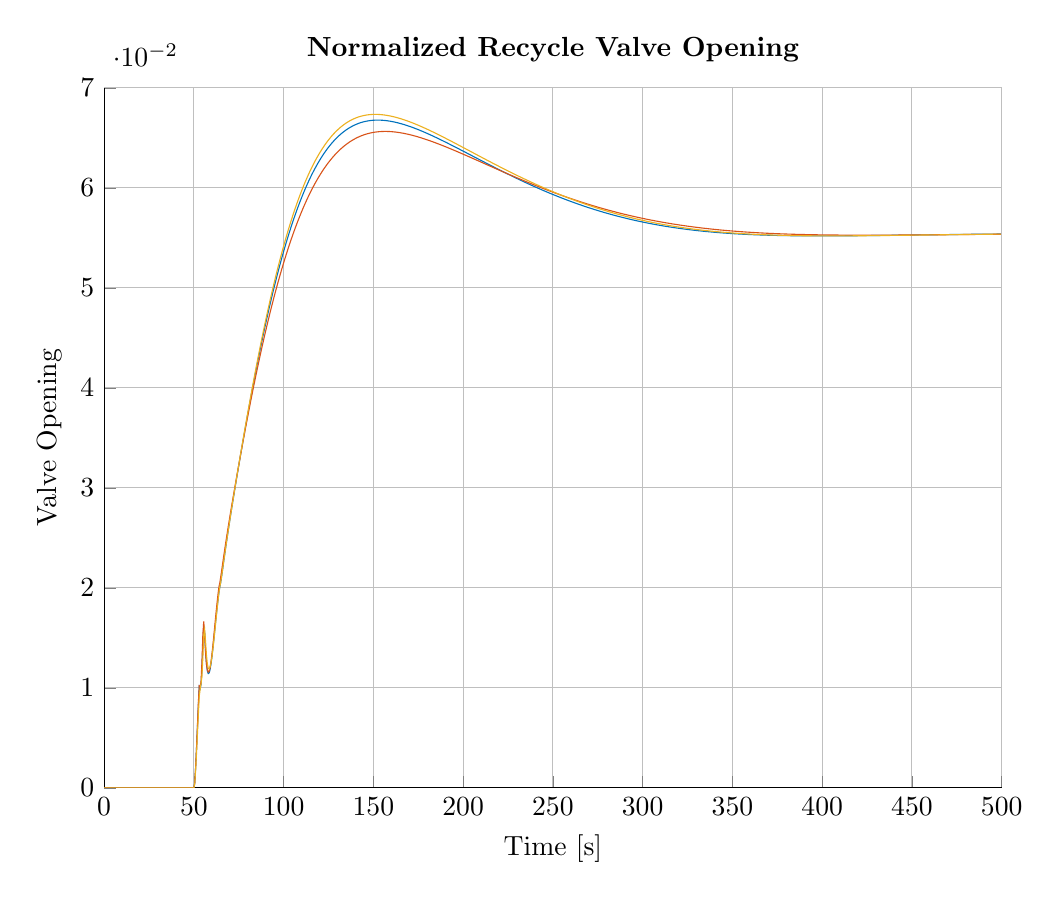
\begin{tikzpicture}

\begin{axis}[%
width=4.488in,
height=3.5in,
at={(0.791in,0.547in)},
scale only axis,
xmin=0,
xmax=500,
xlabel={Time [s]},
xmajorgrids,
ymin=0,
ymax=0.07,
ylabel={Valve Opening},
ymajorgrids,
axis background/.style={fill=white},
title style={font=\bfseries},
title={Normalized Recycle Valve Opening},
axis x line*=bottom,
axis y line*=left
]
\addplot [color=mycolor1,solid,forget plot]
  table[row sep=crcr]{%
0	6.93883000000002e-310\\
0.5	6.93883000000002e-310\\
1	6.93883000000002e-310\\
1.5	6.93883000000002e-310\\
2	6.93883000000002e-310\\
2.5	6.93883000000002e-310\\
3	6.93883000000002e-310\\
3.5	6.93883000000002e-310\\
4	6.93883000000002e-310\\
4.5	6.93883000000002e-310\\
5	6.93883000000002e-310\\
5.5	6.93883000000002e-310\\
6	6.93883000000002e-310\\
6.5	6.93883000000002e-310\\
7	6.93883000000002e-310\\
7.5	6.93883000000002e-310\\
8	6.93883000000002e-310\\
8.5	6.93883000000002e-310\\
9	6.93883000000002e-310\\
9.5	6.93883000000002e-310\\
10	6.93883000000002e-310\\
10.5	6.93883000000002e-310\\
11	6.93883000000002e-310\\
11.5	6.93883000000002e-310\\
12	6.93883000000002e-310\\
12.5	6.93883000000002e-310\\
13	6.93883000000002e-310\\
13.5	6.93883000000002e-310\\
14	6.93883000000002e-310\\
14.5	6.93883000000002e-310\\
15	6.93883000000002e-310\\
15.5	6.93883000000002e-310\\
16	6.93883000000002e-310\\
16.5	6.93883000000002e-310\\
17	6.93883000000002e-310\\
17.5	6.93883000000002e-310\\
18	6.93883000000002e-310\\
18.5	6.93883000000002e-310\\
19	6.93883000000002e-310\\
19.5	6.93883000000002e-310\\
20	6.93883000000002e-310\\
20.5	6.93883000000002e-310\\
21	6.93883000000002e-310\\
21.5	6.93883000000002e-310\\
22	6.93883000000002e-310\\
22.5	6.93883000000002e-310\\
23	6.93883000000002e-310\\
23.5	6.93883000000002e-310\\
24	6.93883000000002e-310\\
24.5	6.93883000000002e-310\\
25	6.93883000000002e-310\\
25.5	6.93883000000002e-310\\
26	6.93883000000002e-310\\
26.5	6.93883000000002e-310\\
27	6.93883000000002e-310\\
27.5	6.93883000000002e-310\\
28	6.93883000000002e-310\\
28.5	6.93883000000002e-310\\
29	6.93883000000002e-310\\
29.5	6.93883000000002e-310\\
30	6.93883000000002e-310\\
30.5	6.93883000000002e-310\\
31	6.93883000000002e-310\\
31.5	6.93883000000002e-310\\
32	6.93883000000002e-310\\
32.5	6.93883000000002e-310\\
33	6.93883000000002e-310\\
33.5	6.93883000000002e-310\\
34	6.93883000000002e-310\\
34.5	6.93883000000002e-310\\
35	6.93883000000002e-310\\
35.5	6.93883000000002e-310\\
36	6.93883000000002e-310\\
36.5	6.93883000000002e-310\\
37	6.93883000000002e-310\\
37.5	6.93883000000002e-310\\
38	6.93883000000002e-310\\
38.5	6.93883000000002e-310\\
39	6.93883000000002e-310\\
39.5	6.93883000000002e-310\\
40	6.93883000000002e-310\\
40.5	6.93883000000002e-310\\
41	6.93883000000002e-310\\
41.5	6.93883000000002e-310\\
42	6.93883000000002e-310\\
42.5	6.93883000000002e-310\\
43	6.93883000000002e-310\\
43.5	6.93883000000002e-310\\
44	6.93883000000002e-310\\
44.5	6.93883000000002e-310\\
45	6.93883000000002e-310\\
45.5	6.93883000000002e-310\\
46	6.93883000000002e-310\\
46.5	6.93883000000002e-310\\
47	6.93883000000002e-310\\
47.5	6.93883000000002e-310\\
48	6.93883000000002e-310\\
48.5	6.93883000000002e-310\\
49	6.93883000000002e-310\\
49.5	6.93883000000002e-310\\
50	6.93883000000002e-310\\
50.5	0.000509304\\
51	0.00211134\\
51.5	0.00400956\\
52	0.00609347\\
52.5	0.00815443\\
53	0.0101092\\
53.5	0.00992427\\
54	0.0103164\\
54.5	0.01186\\
55	0.014282\\
55.5	0.0161968\\
56	0.0155694\\
56.5	0.0137396\\
57	0.0124325\\
57.5	0.0117086\\
58	0.0114301\\
58.5	0.0114875\\
59	0.0118074\\
59.5	0.0123271\\
60	0.0129979\\
60.5	0.0137787\\
61	0.0146315\\
61.5	0.0155202\\
62	0.0164115\\
62.5	0.0172775\\
63	0.0180995\\
63.5	0.0188704\\
64	0.0195952\\
64.5	0.0201304\\
65	0.0205944\\
65.5	0.0211948\\
66	0.0218322\\
66.5	0.0224756\\
67	0.023115\\
67.5	0.023747\\
68	0.0243668\\
68.5	0.0249743\\
69	0.0255706\\
69.5	0.0261569\\
70	0.0267345\\
70.5	0.0273048\\
71	0.0278687\\
71.5	0.0284272\\
72	0.0289809\\
72.5	0.0295304\\
73	0.0300762\\
73.5	0.0306183\\
74	0.0311572\\
74.5	0.0316928\\
75	0.0322253\\
75.5	0.0327546\\
76	0.0332807\\
76.5	0.0338035\\
77	0.0343231\\
77.5	0.0348393\\
78	0.035352\\
78.5	0.0358611\\
79	0.0363666\\
79.5	0.0368684\\
80	0.0373663\\
80.5	0.0378604\\
81	0.0383504\\
81.5	0.0388365\\
82	0.0393184\\
82.5	0.0397961\\
83	0.0402697\\
83.5	0.0407389\\
84	0.0412038\\
84.5	0.0416643\\
85	0.0421204\\
85.5	0.042572\\
86	0.0430191\\
86.5	0.0434617\\
87	0.0438997\\
87.5	0.0443332\\
88	0.044762\\
88.5	0.0451862\\
89	0.0456058\\
89.5	0.0460206\\
90	0.0464308\\
90.5	0.0468363\\
91	0.0472371\\
91.5	0.0476332\\
92	0.0480245\\
92.5	0.0484112\\
93	0.048793\\
93.5	0.0491702\\
94	0.0495426\\
94.5	0.0499103\\
95	0.0502733\\
95.5	0.0506315\\
96	0.050985\\
96.5	0.0513338\\
97	0.0516778\\
97.5	0.0520172\\
98	0.0523519\\
98.5	0.0526819\\
99	0.0530072\\
99.5	0.0533279\\
100	0.0536439\\
100.5	0.0539554\\
101	0.0542622\\
101.5	0.0545644\\
102	0.054862\\
102.5	0.0551551\\
103	0.0554437\\
103.5	0.0557277\\
104	0.0560072\\
104.5	0.0562823\\
105	0.0565529\\
105.5	0.0568191\\
106	0.0570809\\
106.5	0.0573383\\
107	0.0575914\\
107.5	0.0578401\\
108	0.0580846\\
108.5	0.0583247\\
109	0.0585606\\
109.5	0.0587924\\
110	0.0590199\\
110.5	0.0592433\\
111	0.0594625\\
111.5	0.0596777\\
112	0.0598888\\
112.5	0.0600958\\
113	0.0602989\\
113.5	0.060498\\
114	0.0606932\\
114.5	0.0608844\\
115	0.0610718\\
115.5	0.0612554\\
116	0.0614352\\
116.5	0.0616112\\
117	0.0617835\\
117.5	0.0619521\\
118	0.062117\\
118.5	0.0622783\\
119	0.062436\\
119.5	0.0625902\\
120	0.0627409\\
120.5	0.0628881\\
121	0.0630318\\
121.5	0.0631722\\
122	0.0633091\\
122.5	0.0634428\\
123	0.0635732\\
123.5	0.0637003\\
124	0.0638242\\
124.5	0.0639449\\
125	0.0640625\\
125.5	0.064177\\
126	0.0642885\\
126.5	0.0643969\\
127	0.0645023\\
127.5	0.0646048\\
128	0.0647044\\
128.5	0.0648011\\
129	0.064895\\
129.5	0.0649861\\
130	0.0650744\\
130.5	0.06516\\
131	0.0652429\\
131.5	0.0653232\\
132	0.0654009\\
132.5	0.065476\\
133	0.0655486\\
133.5	0.0656186\\
134	0.0656863\\
134.5	0.0657515\\
135	0.0658143\\
135.5	0.0658748\\
136	0.0659329\\
136.5	0.0659888\\
137	0.0660424\\
137.5	0.0660939\\
138	0.0661432\\
138.5	0.0661903\\
139	0.0662353\\
139.5	0.0662783\\
140	0.0663193\\
140.5	0.0663582\\
141	0.0663952\\
141.5	0.0664302\\
142	0.0664634\\
142.5	0.0664947\\
143	0.0665241\\
143.5	0.0665518\\
144	0.0665777\\
144.5	0.0666018\\
145	0.0666243\\
145.5	0.0666451\\
146	0.0666642\\
146.5	0.0666817\\
147	0.0666976\\
147.5	0.066712\\
148	0.0667249\\
148.5	0.0667362\\
149	0.0667461\\
149.5	0.0667546\\
150	0.0667616\\
150.5	0.0667672\\
151	0.0667715\\
151.5	0.0667745\\
152	0.0667761\\
152.5	0.0667765\\
153	0.0667756\\
153.5	0.0667735\\
154	0.0667702\\
154.5	0.0667657\\
155	0.06676\\
155.5	0.0667532\\
156	0.0667453\\
156.5	0.0667363\\
157	0.0667263\\
157.5	0.0667152\\
158	0.0667031\\
158.5	0.06669\\
159	0.0666759\\
159.5	0.0666609\\
160	0.0666449\\
160.5	0.066628\\
161	0.0666103\\
161.5	0.0665916\\
162	0.0665721\\
162.5	0.0665518\\
163	0.0665306\\
163.5	0.0665087\\
164	0.066486\\
164.5	0.0664625\\
165	0.0664382\\
165.5	0.0664133\\
166	0.0663876\\
166.5	0.0663613\\
167	0.0663342\\
167.5	0.0663065\\
168	0.0662782\\
168.5	0.0662492\\
169	0.0662196\\
169.5	0.0661894\\
170	0.0661587\\
170.5	0.0661273\\
171	0.0660954\\
171.5	0.066063\\
172	0.06603\\
172.5	0.0659965\\
173	0.0659626\\
173.5	0.0659281\\
174	0.0658932\\
174.5	0.0658578\\
175	0.0658219\\
175.5	0.0657856\\
176	0.0657489\\
176.5	0.0657118\\
177	0.0656743\\
177.5	0.0656363\\
178	0.065598\\
178.5	0.0655594\\
179	0.0655203\\
179.5	0.065481\\
180	0.0654412\\
180.5	0.0654012\\
181	0.0653608\\
181.5	0.0653202\\
182	0.0652792\\
182.5	0.065238\\
183	0.0651964\\
183.5	0.0651546\\
184	0.0651126\\
184.5	0.0650702\\
185	0.0650277\\
185.5	0.0649849\\
186	0.0649418\\
186.5	0.0648986\\
187	0.0648551\\
187.5	0.0648115\\
188	0.0647676\\
188.5	0.0647236\\
189	0.0646794\\
189.5	0.064635\\
190	0.0645904\\
190.5	0.0645457\\
191	0.0645008\\
191.5	0.0644558\\
192	0.0644106\\
192.5	0.0643653\\
193	0.0643199\\
193.5	0.0642743\\
194	0.0642287\\
194.5	0.0641829\\
195	0.0641371\\
195.5	0.0640911\\
196	0.0640451\\
196.5	0.0639989\\
197	0.0639527\\
197.5	0.0639064\\
198	0.0638601\\
198.5	0.0638136\\
199	0.0637672\\
199.5	0.0637206\\
200	0.0636741\\
200.5	0.0636274\\
201	0.0635808\\
201.5	0.0635341\\
202	0.0634874\\
202.5	0.0634406\\
203	0.0633938\\
203.5	0.0633471\\
204	0.0633003\\
204.5	0.0632535\\
205	0.0632067\\
205.5	0.0631599\\
206	0.0631131\\
206.5	0.0630663\\
207	0.0630195\\
207.5	0.0629727\\
208	0.062926\\
208.5	0.0628793\\
209	0.0628326\\
209.5	0.062786\\
210	0.0627393\\
210.5	0.0626928\\
211	0.0626462\\
211.5	0.0625997\\
212	0.0625533\\
212.5	0.0625069\\
213	0.0624605\\
213.5	0.0624142\\
214	0.062368\\
214.5	0.0623219\\
215	0.0622758\\
215.5	0.0622297\\
216	0.0621838\\
216.5	0.0621379\\
217	0.0620921\\
217.5	0.0620464\\
218	0.0620007\\
218.5	0.0619552\\
219	0.0619097\\
219.5	0.0618643\\
220	0.061819\\
220.5	0.0617738\\
221	0.0617287\\
221.5	0.0616837\\
222	0.0616388\\
222.5	0.061594\\
223	0.0615493\\
223.5	0.0615048\\
224	0.0614603\\
224.5	0.0614159\\
225	0.0613717\\
225.5	0.0613275\\
226	0.0612835\\
226.5	0.0612396\\
227	0.0611959\\
227.5	0.0611522\\
228	0.0611087\\
228.5	0.0610653\\
229	0.061022\\
229.5	0.0609789\\
230	0.0609359\\
230.5	0.060893\\
231	0.0608502\\
231.5	0.0608076\\
232	0.0607652\\
232.5	0.0607228\\
233	0.0606806\\
233.5	0.0606386\\
234	0.0605967\\
234.5	0.0605549\\
235	0.0605133\\
235.5	0.0604719\\
236	0.0604305\\
236.5	0.0603894\\
237	0.0603484\\
237.5	0.0603075\\
238	0.0602668\\
238.5	0.0602262\\
239	0.0601858\\
239.5	0.0601456\\
240	0.0601055\\
240.5	0.0600656\\
241	0.0600258\\
241.5	0.0599862\\
242	0.0599468\\
242.5	0.0599075\\
243	0.0598684\\
243.5	0.0598295\\
244	0.0597907\\
244.5	0.0597521\\
245	0.0597136\\
245.5	0.0596753\\
246	0.0596372\\
246.5	0.0595993\\
247	0.0595615\\
247.5	0.0595239\\
248	0.0594865\\
248.5	0.0594492\\
249	0.0594121\\
249.5	0.0593752\\
250	0.0593385\\
};
\addplot [color=mycolor1,solid,forget plot]
  table[row sep=crcr]{%
250	0.0593385\\
250.5	0.0593019\\
251	0.0592655\\
251.5	0.0592293\\
252	0.0591933\\
252.5	0.0591574\\
253	0.0591218\\
253.5	0.0590863\\
254	0.0590509\\
254.5	0.0590158\\
255	0.0589808\\
255.5	0.0589461\\
256	0.0589115\\
256.5	0.058877\\
257	0.0588428\\
257.5	0.0588087\\
258	0.0587749\\
258.5	0.0587412\\
259	0.0587077\\
259.5	0.0586743\\
260	0.0586412\\
260.5	0.0586082\\
261	0.0585754\\
261.5	0.0585429\\
262	0.0585104\\
262.5	0.0584782\\
263	0.0584462\\
263.5	0.0584143\\
264	0.0583827\\
264.5	0.0583512\\
265	0.0583199\\
265.5	0.0582887\\
266	0.0582578\\
266.5	0.0582271\\
267	0.0581965\\
267.5	0.0581661\\
268	0.0581359\\
268.5	0.0581059\\
269	0.0580761\\
269.5	0.0580465\\
270	0.058017\\
270.5	0.0579878\\
271	0.0579587\\
271.5	0.0579298\\
272	0.0579011\\
272.5	0.0578726\\
273	0.0578442\\
273.5	0.0578161\\
274	0.0577881\\
274.5	0.0577603\\
275	0.0577327\\
275.5	0.0577053\\
276	0.0576781\\
276.5	0.0576511\\
277	0.0576242\\
277.5	0.0575975\\
278	0.057571\\
278.5	0.0575447\\
279	0.0575186\\
279.5	0.0574927\\
280	0.0574669\\
280.5	0.0574413\\
281	0.0574159\\
281.5	0.0573907\\
282	0.0573657\\
282.5	0.0573408\\
283	0.0573162\\
283.5	0.0572917\\
284	0.0572674\\
284.5	0.0572432\\
285	0.0572193\\
285.5	0.0571955\\
286	0.0571719\\
286.5	0.0571485\\
287	0.0571253\\
287.5	0.0571022\\
288	0.0570794\\
288.5	0.0570567\\
289	0.0570341\\
289.5	0.0570118\\
290	0.0569896\\
290.5	0.0569676\\
291	0.0569458\\
291.5	0.0569241\\
292	0.0569027\\
292.5	0.0568814\\
293	0.0568603\\
293.5	0.0568393\\
294	0.0568185\\
294.5	0.0567979\\
295	0.0567775\\
295.5	0.0567572\\
296	0.0567371\\
296.5	0.0567172\\
297	0.0566974\\
297.5	0.0566778\\
298	0.0566584\\
298.5	0.0566392\\
299	0.0566201\\
299.5	0.0566011\\
300	0.0565824\\
300.5	0.0565638\\
301	0.0565454\\
301.5	0.0565271\\
302	0.056509\\
302.5	0.0564911\\
303	0.0564733\\
303.5	0.0564557\\
304	0.0564382\\
304.5	0.056421\\
305	0.0564038\\
305.5	0.0563869\\
306	0.05637\\
306.5	0.0563534\\
307	0.0563369\\
307.5	0.0563205\\
308	0.0563044\\
308.5	0.0562883\\
309	0.0562725\\
309.5	0.0562567\\
310	0.0562412\\
310.5	0.0562258\\
311	0.0562105\\
311.5	0.0561954\\
312	0.0561804\\
312.5	0.0561656\\
313	0.0561509\\
313.5	0.0561364\\
314	0.056122\\
314.5	0.0561078\\
315	0.0560938\\
315.5	0.0560798\\
316	0.056066\\
316.5	0.0560524\\
317	0.0560389\\
317.5	0.0560255\\
318	0.0560123\\
318.5	0.0559993\\
319	0.0559863\\
319.5	0.0559735\\
320	0.0559609\\
320.5	0.0559484\\
321	0.055936\\
321.5	0.0559238\\
322	0.0559116\\
322.5	0.0558997\\
323	0.0558878\\
323.5	0.0558761\\
324	0.0558646\\
324.5	0.0558531\\
325	0.0558418\\
325.5	0.0558307\\
326	0.0558196\\
326.5	0.0558087\\
327	0.0557979\\
327.5	0.0557872\\
328	0.0557767\\
328.5	0.0557663\\
329	0.055756\\
329.5	0.0557459\\
330	0.0557358\\
330.5	0.0557259\\
331	0.0557161\\
331.5	0.0557065\\
332	0.0556969\\
332.5	0.0556875\\
333	0.0556782\\
333.5	0.055669\\
334	0.0556599\\
334.5	0.0556509\\
335	0.0556421\\
335.5	0.0556334\\
336	0.0556248\\
336.5	0.0556163\\
337	0.0556079\\
337.5	0.0555996\\
338	0.0555914\\
338.5	0.0555834\\
339	0.0555754\\
339.5	0.0555676\\
340	0.0555599\\
340.5	0.0555523\\
341	0.0555447\\
341.5	0.0555373\\
342	0.05553\\
342.5	0.0555228\\
343	0.0555157\\
343.5	0.0555087\\
344	0.0555018\\
344.5	0.055495\\
345	0.0554884\\
345.5	0.0554818\\
346	0.0554753\\
346.5	0.0554689\\
347	0.0554626\\
347.5	0.0554564\\
348	0.0554503\\
348.5	0.0554442\\
349	0.0554383\\
349.5	0.0554325\\
350	0.0554268\\
350.5	0.0554211\\
351	0.0554156\\
351.5	0.0554101\\
352	0.0554047\\
352.5	0.0553994\\
353	0.0553942\\
353.5	0.0553891\\
354	0.0553841\\
354.5	0.0553792\\
355	0.0553743\\
355.5	0.0553695\\
356	0.0553648\\
356.5	0.0553602\\
357	0.0553557\\
357.5	0.0553513\\
358	0.0553469\\
358.5	0.0553426\\
359	0.0553384\\
359.5	0.0553343\\
360	0.0553302\\
360.5	0.0553263\\
361	0.0553224\\
361.5	0.0553186\\
362	0.0553148\\
362.5	0.0553111\\
363	0.0553075\\
363.5	0.055304\\
364	0.0553006\\
364.5	0.0552972\\
365	0.0552939\\
365.5	0.0552906\\
366	0.0552874\\
366.5	0.0552843\\
367	0.0552813\\
367.5	0.0552783\\
368	0.0552754\\
368.5	0.0552725\\
369	0.0552698\\
369.5	0.0552671\\
370	0.0552644\\
370.5	0.0552618\\
371	0.0552593\\
371.5	0.0552568\\
372	0.0552544\\
372.5	0.0552521\\
373	0.0552498\\
373.5	0.0552475\\
374	0.0552454\\
374.5	0.0552433\\
375	0.0552412\\
375.5	0.0552392\\
376	0.0552373\\
376.5	0.0552354\\
377	0.0552335\\
377.5	0.0552318\\
378	0.05523\\
378.5	0.0552283\\
379	0.0552267\\
379.5	0.0552251\\
380	0.0552236\\
380.5	0.0552221\\
381	0.0552207\\
381.5	0.0552193\\
382	0.055218\\
382.5	0.0552167\\
383	0.0552155\\
383.5	0.0552143\\
384	0.0552132\\
384.5	0.0552121\\
385	0.055211\\
385.5	0.05521\\
386	0.055209\\
386.5	0.0552081\\
387	0.0552072\\
387.5	0.0552064\\
388	0.0552056\\
388.5	0.0552048\\
389	0.0552041\\
389.5	0.0552035\\
390	0.0552028\\
390.5	0.0552022\\
391	0.0552017\\
391.5	0.0552011\\
392	0.0552006\\
392.5	0.0552002\\
393	0.0551998\\
393.5	0.0551994\\
394	0.055199\\
394.5	0.0551987\\
395	0.0551985\\
395.5	0.0551982\\
396	0.055198\\
396.5	0.0551978\\
397	0.0551977\\
397.5	0.0551976\\
398	0.0551975\\
398.5	0.0551974\\
399	0.0551974\\
399.5	0.0551974\\
400	0.0551974\\
400.5	0.0551975\\
401	0.0551976\\
401.5	0.0551977\\
402	0.0551978\\
402.5	0.055198\\
403	0.0551982\\
403.5	0.0551984\\
404	0.0551987\\
404.5	0.055199\\
405	0.0551993\\
405.5	0.0551996\\
406	0.0551999\\
406.5	0.0552003\\
407	0.0552007\\
407.5	0.0552011\\
408	0.0552016\\
408.5	0.055202\\
409	0.0552025\\
409.5	0.055203\\
410	0.0552035\\
410.5	0.0552041\\
411	0.0552046\\
411.5	0.0552052\\
412	0.0552058\\
412.5	0.0552064\\
413	0.0552071\\
413.5	0.0552077\\
414	0.0552084\\
414.5	0.0552091\\
415	0.0552098\\
415.5	0.0552105\\
416	0.0552113\\
416.5	0.055212\\
417	0.0552128\\
417.5	0.0552136\\
418	0.0552144\\
418.5	0.0552152\\
419	0.055216\\
419.5	0.0552169\\
420	0.0552177\\
420.5	0.0552186\\
421	0.0552195\\
421.5	0.0552204\\
422	0.0552213\\
422.5	0.0552222\\
423	0.0552231\\
423.5	0.0552241\\
424	0.055225\\
424.5	0.055226\\
425	0.0552269\\
425.5	0.0552279\\
426	0.0552289\\
426.5	0.0552299\\
427	0.0552309\\
427.5	0.055232\\
428	0.055233\\
428.5	0.055234\\
429	0.0552351\\
429.5	0.0552361\\
430	0.0552372\\
430.5	0.0552383\\
431	0.0552393\\
431.5	0.0552404\\
432	0.0552415\\
432.5	0.0552426\\
433	0.0552437\\
433.5	0.0552448\\
434	0.055246\\
434.5	0.0552471\\
435	0.0552482\\
435.5	0.0552493\\
436	0.0552505\\
436.5	0.0552516\\
437	0.0552528\\
437.5	0.0552539\\
438	0.0552551\\
438.5	0.0552562\\
439	0.0552574\\
439.5	0.0552586\\
440	0.0552597\\
440.5	0.0552609\\
441	0.0552621\\
441.5	0.0552633\\
442	0.0552644\\
442.5	0.0552656\\
443	0.0552668\\
443.5	0.055268\\
444	0.0552692\\
444.5	0.0552704\\
445	0.0552716\\
445.5	0.0552728\\
446	0.0552739\\
446.5	0.0552751\\
447	0.0552763\\
447.5	0.0552775\\
448	0.0552787\\
448.5	0.0552799\\
449	0.0552811\\
449.5	0.0552823\\
450	0.0552835\\
450.5	0.0552847\\
451	0.0552859\\
451.5	0.0552871\\
452	0.0552883\\
452.5	0.0552895\\
453	0.0552907\\
453.5	0.0552919\\
454	0.0552931\\
454.5	0.0552943\\
455	0.0552954\\
455.5	0.0552966\\
456	0.0552978\\
456.5	0.055299\\
457	0.0553002\\
457.5	0.0553014\\
458	0.0553025\\
458.5	0.0553037\\
459	0.0553049\\
459.5	0.0553061\\
460	0.0553072\\
460.5	0.0553084\\
461	0.0553095\\
461.5	0.0553107\\
462	0.0553119\\
462.5	0.055313\\
463	0.0553142\\
463.5	0.0553153\\
464	0.0553164\\
464.5	0.0553176\\
465	0.0553187\\
465.5	0.0553199\\
466	0.055321\\
466.5	0.0553221\\
467	0.0553232\\
467.5	0.0553243\\
468	0.0553254\\
468.5	0.0553266\\
469	0.0553277\\
469.5	0.0553288\\
470	0.0553299\\
470.5	0.0553309\\
471	0.055332\\
471.5	0.0553331\\
472	0.0553342\\
472.5	0.0553353\\
473	0.0553363\\
473.5	0.0553374\\
474	0.0553385\\
474.5	0.0553395\\
475	0.0553406\\
475.5	0.0553416\\
476	0.0553426\\
476.5	0.0553437\\
477	0.0553447\\
477.5	0.0553457\\
478	0.0553467\\
478.5	0.0553478\\
479	0.0553488\\
479.5	0.0553498\\
480	0.0553508\\
480.5	0.0553518\\
481	0.0553527\\
481.5	0.0553537\\
482	0.0553547\\
482.5	0.0553557\\
483	0.0553566\\
483.5	0.0553576\\
484	0.0553585\\
484.5	0.0553595\\
485	0.0553604\\
485.5	0.0553614\\
486	0.0553623\\
486.5	0.0553632\\
487	0.0553641\\
487.5	0.055365\\
488	0.055366\\
488.5	0.0553669\\
489	0.0553678\\
489.5	0.0553686\\
490	0.0553695\\
490.5	0.0553704\\
491	0.0553713\\
491.5	0.0553721\\
492	0.055373\\
492.5	0.0553739\\
493	0.0553747\\
493.5	0.0553755\\
494	0.0553764\\
494.5	0.0553772\\
495	0.055378\\
495.5	0.0553789\\
496	0.0553797\\
496.5	0.0553805\\
497	0.0553813\\
497.5	0.0553821\\
498	0.0553828\\
498.5	0.0553836\\
499	0.0553844\\
499.5	0.0553852\\
};
\addplot [color=mycolor2,solid,forget plot]
  table[row sep=crcr]{%
0	6.91844e-310\\
0.5	6.91844e-310\\
1	6.91844e-310\\
1.5	6.91844e-310\\
2	6.91844e-310\\
2.5	6.91844e-310\\
3	6.91844e-310\\
3.5	6.91844e-310\\
4	6.91844e-310\\
4.5	6.91844e-310\\
5	6.91844e-310\\
5.5	6.91844e-310\\
6	6.91844e-310\\
6.5	6.91844e-310\\
7	6.91844e-310\\
7.5	6.91844e-310\\
8	6.91844e-310\\
8.5	6.91844e-310\\
9	6.91844e-310\\
9.5	6.91844e-310\\
10	6.91844e-310\\
10.5	6.91844e-310\\
11	6.91844e-310\\
11.5	6.91844e-310\\
12	6.91844e-310\\
12.5	6.91844e-310\\
13	6.91844e-310\\
13.5	6.91844e-310\\
14	6.91844e-310\\
14.5	6.91844e-310\\
15	6.91844e-310\\
15.5	6.91844e-310\\
16	6.91844e-310\\
16.5	6.91844e-310\\
17	6.91844e-310\\
17.5	6.91844e-310\\
18	6.91844e-310\\
18.5	6.91844e-310\\
19	6.91844e-310\\
19.5	6.91844e-310\\
20	6.91844e-310\\
20.5	6.91844e-310\\
21	6.91844e-310\\
21.5	6.91844e-310\\
22	6.91844e-310\\
22.5	6.91844e-310\\
23	6.91844e-310\\
23.5	6.91844e-310\\
24	6.91844e-310\\
24.5	6.91844e-310\\
25	6.91844e-310\\
25.5	6.91844e-310\\
26	6.91844e-310\\
26.5	6.91844e-310\\
27	6.91844e-310\\
27.5	6.91844e-310\\
28	6.91844e-310\\
28.5	6.91844e-310\\
29	6.91844e-310\\
29.5	6.91844e-310\\
30	6.91844e-310\\
30.5	6.91844e-310\\
31	6.91844e-310\\
31.5	6.91844e-310\\
32	6.91844e-310\\
32.5	6.91844e-310\\
33	6.91844e-310\\
33.5	6.91844e-310\\
34	6.91844e-310\\
34.5	6.91844e-310\\
35	6.91844e-310\\
35.5	6.91844e-310\\
36	6.91844e-310\\
36.5	6.91844e-310\\
37	6.91844e-310\\
37.5	6.91844e-310\\
38	6.91844e-310\\
38.5	6.91844e-310\\
39	6.91844e-310\\
39.5	6.91844e-310\\
40	6.91844e-310\\
40.5	6.91844e-310\\
41	6.91844e-310\\
41.5	6.91844e-310\\
42	6.91844e-310\\
42.5	6.91844e-310\\
43	6.91844e-310\\
43.5	6.91844e-310\\
44	6.91844e-310\\
44.5	6.91844e-310\\
45	6.91844e-310\\
45.5	6.91844e-310\\
46	6.91844e-310\\
46.5	6.91844e-310\\
47	6.91844e-310\\
47.5	6.91844e-310\\
48	6.91844e-310\\
48.5	6.91844e-310\\
49	6.91844e-310\\
49.5	6.91844e-310\\
50	6.91844e-310\\
50.5	0.000522473\\
51	0.00216432\\
51.5	0.00412168\\
52	0.00630136\\
52.5	0.00850739\\
53	0.0101892\\
53.5	0.0101035\\
54	0.0106601\\
54.5	0.0125997\\
55	0.0152694\\
55.5	0.0166539\\
56	0.0152726\\
56.5	0.0135382\\
57	0.0124146\\
57.5	0.0118055\\
58	0.0115739\\
58.5	0.0116558\\
59	0.0119993\\
59.5	0.0125482\\
60	0.0132555\\
60.5	0.0140792\\
61	0.0149794\\
61.5	0.0159176\\
62	0.0168581\\
62.5	0.0177707\\
63	0.0186351\\
63.5	0.0194435\\
64	0.0201151\\
64.5	0.0205489\\
65	0.021133\\
65.5	0.0217541\\
66	0.0223797\\
66.5	0.0229991\\
67	0.0236135\\
67.5	0.0242172\\
68	0.0248089\\
68.5	0.0253888\\
69	0.0259578\\
69.5	0.0265171\\
70	0.0270678\\
70.5	0.0276109\\
71	0.0281477\\
71.5	0.0286788\\
72	0.029205\\
72.5	0.0297268\\
73	0.0302448\\
73.5	0.0307591\\
74	0.03127\\
74.5	0.0317777\\
75	0.0322821\\
75.5	0.0327834\\
76	0.0332815\\
76.5	0.0337764\\
77	0.034268\\
77.5	0.0347562\\
78	0.0352411\\
78.5	0.0357224\\
79	0.0362002\\
79.5	0.0366744\\
80	0.0371448\\
80.5	0.0376114\\
81	0.0380742\\
81.5	0.0385331\\
82	0.038988\\
82.5	0.0394389\\
83	0.0398856\\
83.5	0.0403283\\
84	0.0407668\\
84.5	0.0412011\\
85	0.0416312\\
85.5	0.042057\\
86	0.0424785\\
86.5	0.0428957\\
87	0.0433085\\
87.5	0.043717\\
88	0.0441212\\
88.5	0.0445209\\
89	0.0449162\\
89.5	0.0453071\\
90	0.0456936\\
90.5	0.0460757\\
91	0.0464533\\
91.5	0.0468265\\
92	0.0471953\\
92.5	0.0475596\\
93	0.0479195\\
93.5	0.048275\\
94	0.048626\\
94.5	0.0489727\\
95	0.0493149\\
95.5	0.0496528\\
96	0.0499862\\
96.5	0.0503153\\
97	0.05064\\
97.5	0.0509604\\
98	0.0512764\\
98.5	0.0515881\\
99	0.0518955\\
99.5	0.0521986\\
100	0.0524975\\
100.5	0.0527921\\
101	0.0530824\\
101.5	0.0533686\\
102	0.0536505\\
102.5	0.0539283\\
103	0.0542019\\
103.5	0.0544714\\
104	0.0547368\\
104.5	0.0549981\\
105	0.0552553\\
105.5	0.0555086\\
106	0.0557578\\
106.5	0.056003\\
107	0.0562443\\
107.5	0.0564816\\
108	0.056715\\
108.5	0.0569446\\
109	0.0571703\\
109.5	0.0573922\\
110	0.0576103\\
110.5	0.0578246\\
111	0.0580352\\
111.5	0.0582421\\
112	0.0584453\\
112.5	0.0586448\\
113	0.0588408\\
113.5	0.0590331\\
114	0.0592219\\
114.5	0.0594072\\
115	0.0595889\\
115.5	0.0597673\\
116	0.0599421\\
116.5	0.0601136\\
117	0.0602817\\
117.5	0.0604465\\
118	0.0606079\\
118.5	0.0607661\\
119	0.0609211\\
119.5	0.0610728\\
120	0.0612214\\
120.5	0.0613668\\
121	0.0615091\\
121.5	0.0616483\\
122	0.0617845\\
122.5	0.0619177\\
123	0.0620479\\
123.5	0.0621751\\
124	0.0622994\\
124.5	0.0624209\\
125	0.0625395\\
125.5	0.0626553\\
126	0.0627683\\
126.5	0.0628785\\
127	0.0629861\\
127.5	0.0630909\\
128	0.0631931\\
128.5	0.0632927\\
129	0.0633897\\
129.5	0.0634842\\
130	0.0635761\\
130.5	0.0636656\\
131	0.0637526\\
131.5	0.0638372\\
132	0.0639194\\
132.5	0.0639992\\
133	0.0640767\\
133.5	0.0641519\\
134	0.0642249\\
134.5	0.0642956\\
135	0.0643641\\
135.5	0.0644305\\
136	0.0644947\\
136.5	0.0645568\\
137	0.0646169\\
137.5	0.0646749\\
138	0.0647309\\
138.5	0.0647849\\
139	0.0648369\\
139.5	0.0648871\\
140	0.0649353\\
140.5	0.0649817\\
141	0.0650262\\
141.5	0.065069\\
142	0.06511\\
142.5	0.0651492\\
143	0.0651867\\
143.5	0.0652225\\
144	0.0652566\\
144.5	0.0652891\\
145	0.06532\\
145.5	0.0653493\\
146	0.065377\\
146.5	0.0654033\\
147	0.065428\\
147.5	0.0654512\\
148	0.065473\\
148.5	0.0654933\\
149	0.0655123\\
149.5	0.0655299\\
150	0.0655461\\
150.5	0.065561\\
151	0.0655746\\
151.5	0.0655869\\
152	0.0655979\\
152.5	0.0656077\\
153	0.0656163\\
153.5	0.0656237\\
154	0.06563\\
154.5	0.0656351\\
155	0.0656391\\
155.5	0.0656419\\
156	0.0656437\\
156.5	0.0656444\\
157	0.0656441\\
157.5	0.0656428\\
158	0.0656404\\
158.5	0.0656371\\
159	0.0656328\\
159.5	0.0656276\\
160	0.0656215\\
160.5	0.0656144\\
161	0.0656065\\
161.5	0.0655976\\
162	0.065588\\
162.5	0.0655775\\
163	0.0655662\\
163.5	0.065554\\
164	0.0655411\\
164.5	0.0655275\\
165	0.0655131\\
165.5	0.0654979\\
166	0.065482\\
166.5	0.0654655\\
167	0.0654482\\
167.5	0.0654303\\
168	0.0654117\\
168.5	0.0653924\\
169	0.0653725\\
169.5	0.0653521\\
170	0.065331\\
170.5	0.0653093\\
171	0.065287\\
171.5	0.0652642\\
172	0.0652408\\
172.5	0.0652169\\
173	0.0651925\\
173.5	0.0651676\\
174	0.0651421\\
174.5	0.0651162\\
175	0.0650898\\
175.5	0.0650629\\
176	0.0650356\\
176.5	0.0650078\\
177	0.0649796\\
177.5	0.064951\\
178	0.0649219\\
178.5	0.0648925\\
179	0.0648627\\
179.5	0.0648325\\
180	0.0648019\\
180.5	0.0647709\\
181	0.0647396\\
181.5	0.064708\\
182	0.064676\\
182.5	0.0646437\\
183	0.0646111\\
183.5	0.0645782\\
184	0.064545\\
184.5	0.0645115\\
185	0.0644777\\
185.5	0.0644437\\
186	0.0644094\\
186.5	0.0643748\\
187	0.06434\\
187.5	0.0643049\\
188	0.0642696\\
188.5	0.064234\\
189	0.0641983\\
189.5	0.0641623\\
190	0.0641262\\
190.5	0.0640898\\
191	0.0640532\\
191.5	0.0640165\\
192	0.0639795\\
192.5	0.0639424\\
193	0.0639052\\
193.5	0.0638677\\
194	0.0638302\\
194.5	0.0637924\\
195	0.0637545\\
195.5	0.0637165\\
196	0.0636784\\
196.5	0.0636401\\
197	0.0636017\\
197.5	0.0635632\\
198	0.0635246\\
198.5	0.0634858\\
199	0.063447\\
199.5	0.0634081\\
200	0.0633691\\
200.5	0.06333\\
201	0.0632908\\
201.5	0.0632515\\
202	0.0632122\\
202.5	0.0631728\\
203	0.0631333\\
203.5	0.0630938\\
204	0.0630542\\
204.5	0.0630146\\
205	0.062975\\
205.5	0.0629352\\
206	0.0628955\\
206.5	0.0628557\\
207	0.0628159\\
207.5	0.062776\\
208	0.0627362\\
208.5	0.0626963\\
209	0.0626564\\
209.5	0.0626165\\
210	0.0625766\\
210.5	0.0625366\\
211	0.0624967\\
211.5	0.0624568\\
212	0.0624168\\
212.5	0.0623769\\
213	0.062337\\
213.5	0.0622971\\
214	0.0622572\\
214.5	0.0622174\\
215	0.0621775\\
215.5	0.0621377\\
216	0.0620979\\
216.5	0.0620582\\
217	0.0620184\\
217.5	0.0619787\\
218	0.0619391\\
218.5	0.0618995\\
219	0.0618599\\
219.5	0.0618204\\
220	0.0617809\\
220.5	0.0617415\\
221	0.0617021\\
221.5	0.0616628\\
222	0.0616235\\
222.5	0.0615843\\
223	0.0615452\\
223.5	0.0615061\\
224	0.0614671\\
224.5	0.0614282\\
225	0.0613893\\
225.5	0.0613505\\
226	0.0613118\\
226.5	0.0612731\\
227	0.0612345\\
227.5	0.061196\\
228	0.0611576\\
228.5	0.0611193\\
229	0.0610811\\
229.5	0.0610429\\
230	0.0610048\\
230.5	0.0609668\\
231	0.0609289\\
231.5	0.0608911\\
232	0.0608534\\
232.5	0.0608158\\
233	0.0607783\\
233.5	0.0607409\\
234	0.0607036\\
234.5	0.0606664\\
235	0.0606293\\
235.5	0.0605923\\
236	0.0605554\\
236.5	0.0605186\\
237	0.0604819\\
237.5	0.0604453\\
238	0.0604088\\
238.5	0.0603725\\
239	0.0603362\\
239.5	0.0603001\\
240	0.0602641\\
240.5	0.0602282\\
241	0.0601924\\
241.5	0.0601568\\
242	0.0601212\\
242.5	0.0600858\\
243	0.0600505\\
243.5	0.0600153\\
244	0.0599803\\
244.5	0.0599453\\
245	0.0599105\\
245.5	0.0598759\\
246	0.0598413\\
246.5	0.0598069\\
247	0.0597726\\
247.5	0.0597384\\
248	0.0597044\\
248.5	0.0596705\\
249	0.0596367\\
249.5	0.0596031\\
250	0.0595696\\
};
\addplot [color=mycolor2,solid,forget plot]
  table[row sep=crcr]{%
250	0.0595696\\
250.5	0.0595362\\
251	0.059503\\
251.5	0.0594699\\
252	0.0594369\\
252.5	0.0594041\\
253	0.0593714\\
253.5	0.0593388\\
254	0.0593064\\
254.5	0.0592741\\
255	0.059242\\
255.5	0.05921\\
256	0.0591781\\
256.5	0.0591464\\
257	0.0591148\\
257.5	0.0590834\\
258	0.0590521\\
258.5	0.0590209\\
259	0.0589899\\
259.5	0.058959\\
260	0.0589283\\
260.5	0.0588977\\
261	0.0588673\\
261.5	0.058837\\
262	0.0588069\\
262.5	0.0587769\\
263	0.058747\\
263.5	0.0587173\\
264	0.0586878\\
264.5	0.0586584\\
265	0.0586291\\
265.5	0.0586\\
266	0.058571\\
266.5	0.0585422\\
267	0.0585135\\
267.5	0.058485\\
268	0.0584566\\
268.5	0.0584284\\
269	0.0584003\\
269.5	0.0583724\\
270	0.0583446\\
270.5	0.0583169\\
271	0.0582895\\
271.5	0.0582621\\
272	0.0582349\\
272.5	0.0582079\\
273	0.058181\\
273.5	0.0581543\\
274	0.0581277\\
274.5	0.0581012\\
275	0.058075\\
275.5	0.0580488\\
276	0.0580228\\
276.5	0.057997\\
277	0.0579713\\
277.5	0.0579458\\
278	0.0579204\\
278.5	0.0578951\\
279	0.05787\\
279.5	0.0578451\\
280	0.0578203\\
280.5	0.0577957\\
281	0.0577712\\
281.5	0.0577468\\
282	0.0577226\\
282.5	0.0576986\\
283	0.0576747\\
283.5	0.057651\\
284	0.0576274\\
284.5	0.0576039\\
285	0.0575806\\
285.5	0.0575575\\
286	0.0575345\\
286.5	0.0575116\\
287	0.0574889\\
287.5	0.0574663\\
288	0.0574439\\
288.5	0.0574216\\
289	0.0573995\\
289.5	0.0573776\\
290	0.0573557\\
290.5	0.057334\\
291	0.0573125\\
291.5	0.0572911\\
292	0.0572699\\
292.5	0.0572488\\
293	0.0572278\\
293.5	0.057207\\
294	0.0571864\\
294.5	0.0571658\\
295	0.0571455\\
295.5	0.0571252\\
296	0.0571051\\
296.5	0.0570852\\
297	0.0570654\\
297.5	0.0570457\\
298	0.0570262\\
298.5	0.0570068\\
299	0.0569876\\
299.5	0.0569685\\
300	0.0569496\\
300.5	0.0569307\\
301	0.0569121\\
301.5	0.0568935\\
302	0.0568751\\
302.5	0.0568569\\
303	0.0568388\\
303.5	0.0568208\\
304	0.0568029\\
304.5	0.0567852\\
305	0.0567677\\
305.5	0.0567502\\
306	0.0567329\\
306.5	0.0567158\\
307	0.0566988\\
307.5	0.0566819\\
308	0.0566651\\
308.5	0.0566485\\
309	0.056632\\
309.5	0.0566156\\
310	0.0565994\\
310.5	0.0565833\\
311	0.0565674\\
311.5	0.0565515\\
312	0.0565358\\
312.5	0.0565203\\
313	0.0565048\\
313.5	0.0564895\\
314	0.0564743\\
314.5	0.0564593\\
315	0.0564444\\
315.5	0.0564296\\
316	0.0564149\\
316.5	0.0564003\\
317	0.0563859\\
317.5	0.0563716\\
318	0.0563575\\
318.5	0.0563434\\
319	0.0563295\\
319.5	0.0563157\\
320	0.056302\\
320.5	0.0562885\\
321	0.056275\\
321.5	0.0562617\\
322	0.0562485\\
322.5	0.0562355\\
323	0.0562225\\
323.5	0.0562097\\
324	0.056197\\
324.5	0.0561844\\
325	0.0561719\\
325.5	0.0561595\\
326	0.0561473\\
326.5	0.0561352\\
327	0.0561232\\
327.5	0.0561113\\
328	0.0560995\\
328.5	0.0560878\\
329	0.0560762\\
329.5	0.0560648\\
330	0.0560535\\
330.5	0.0560422\\
331	0.0560311\\
331.5	0.0560201\\
332	0.0560092\\
332.5	0.0559984\\
333	0.0559878\\
333.5	0.0559772\\
334	0.0559667\\
334.5	0.0559564\\
335	0.0559461\\
335.5	0.055936\\
336	0.0559259\\
336.5	0.055916\\
337	0.0559062\\
337.5	0.0558964\\
338	0.0558868\\
338.5	0.0558773\\
339	0.0558679\\
339.5	0.0558585\\
340	0.0558493\\
340.5	0.0558402\\
341	0.0558312\\
341.5	0.0558223\\
342	0.0558134\\
342.5	0.0558047\\
343	0.0557961\\
343.5	0.0557875\\
344	0.0557791\\
344.5	0.0557707\\
345	0.0557625\\
345.5	0.0557543\\
346	0.0557463\\
346.5	0.0557383\\
347	0.0557304\\
347.5	0.0557226\\
348	0.0557149\\
348.5	0.0557073\\
349	0.0556998\\
349.5	0.0556924\\
350	0.055685\\
350.5	0.0556778\\
351	0.0556706\\
351.5	0.0556635\\
352	0.0556565\\
352.5	0.0556496\\
353	0.0556428\\
353.5	0.055636\\
354	0.0556294\\
354.5	0.0556228\\
355	0.0556163\\
355.5	0.0556099\\
356	0.0556036\\
356.5	0.0555973\\
357	0.0555911\\
357.5	0.0555851\\
358	0.055579\\
358.5	0.0555731\\
359	0.0555673\\
359.5	0.0555615\\
360	0.0555558\\
360.5	0.0555502\\
361	0.0555446\\
361.5	0.0555391\\
362	0.0555337\\
362.5	0.0555284\\
363	0.0555232\\
363.5	0.055518\\
364	0.0555129\\
364.5	0.0555078\\
365	0.0555029\\
365.5	0.055498\\
366	0.0554931\\
366.5	0.0554884\\
367	0.0554837\\
367.5	0.0554791\\
368	0.0554745\\
368.5	0.05547\\
369	0.0554656\\
369.5	0.0554613\\
370	0.055457\\
370.5	0.0554527\\
371	0.0554486\\
371.5	0.0554445\\
372	0.0554405\\
372.5	0.0554365\\
373	0.0554326\\
373.5	0.0554287\\
374	0.0554249\\
374.5	0.0554212\\
375	0.0554176\\
375.5	0.055414\\
376	0.0554104\\
376.5	0.0554069\\
377	0.0554035\\
377.5	0.0554001\\
378	0.0553968\\
378.5	0.0553935\\
379	0.0553903\\
379.5	0.0553872\\
380	0.0553841\\
380.5	0.055381\\
381	0.055378\\
381.5	0.0553751\\
382	0.0553722\\
382.5	0.0553694\\
383	0.0553666\\
383.5	0.0553639\\
384	0.0553612\\
384.5	0.0553586\\
385	0.055356\\
385.5	0.0553535\\
386	0.055351\\
386.5	0.0553486\\
387	0.0553462\\
387.5	0.0553439\\
388	0.0553416\\
388.5	0.0553393\\
389	0.0553371\\
389.5	0.055335\\
390	0.0553329\\
390.5	0.0553308\\
391	0.0553288\\
391.5	0.0553268\\
392	0.0553249\\
392.5	0.055323\\
393	0.0553211\\
393.5	0.0553193\\
394	0.0553176\\
394.5	0.0553158\\
395	0.0553142\\
395.5	0.0553125\\
396	0.0553109\\
396.5	0.0553093\\
397	0.0553078\\
397.5	0.0553063\\
398	0.0553049\\
398.5	0.0553035\\
399	0.0553021\\
399.5	0.0553007\\
400	0.0552994\\
400.5	0.0552982\\
401	0.0552969\\
401.5	0.0552957\\
402	0.0552946\\
402.5	0.0552934\\
403	0.0552923\\
403.5	0.0552913\\
404	0.0552903\\
404.5	0.0552893\\
405	0.0552883\\
405.5	0.0552874\\
406	0.0552864\\
406.5	0.0552856\\
407	0.0552847\\
407.5	0.0552839\\
408	0.0552831\\
408.5	0.0552824\\
409	0.0552817\\
409.5	0.055281\\
410	0.0552803\\
410.5	0.0552796\\
411	0.055279\\
411.5	0.0552785\\
412	0.0552779\\
412.5	0.0552774\\
413	0.0552769\\
413.5	0.0552764\\
414	0.0552759\\
414.5	0.0552755\\
415	0.0552751\\
415.5	0.0552747\\
416	0.0552743\\
416.5	0.055274\\
417	0.0552737\\
417.5	0.0552734\\
418	0.0552731\\
418.5	0.0552729\\
419	0.0552727\\
419.5	0.0552725\\
420	0.0552723\\
420.5	0.0552721\\
421	0.055272\\
421.5	0.0552719\\
422	0.0552718\\
422.5	0.0552717\\
423	0.0552717\\
423.5	0.0552716\\
424	0.0552716\\
424.5	0.0552716\\
425	0.0552716\\
425.5	0.0552717\\
426	0.0552717\\
426.5	0.0552718\\
427	0.0552719\\
427.5	0.055272\\
428	0.0552721\\
428.5	0.0552722\\
429	0.0552724\\
429.5	0.0552726\\
430	0.0552727\\
430.5	0.055273\\
431	0.0552732\\
431.5	0.0552734\\
432	0.0552736\\
432.5	0.0552739\\
433	0.0552742\\
433.5	0.0552745\\
434	0.0552748\\
434.5	0.0552751\\
435	0.0552754\\
435.5	0.0552758\\
436	0.0552761\\
436.5	0.0552765\\
437	0.0552769\\
437.5	0.0552772\\
438	0.0552776\\
438.5	0.0552781\\
439	0.0552785\\
439.5	0.0552789\\
440	0.0552794\\
440.5	0.0552798\\
441	0.0552803\\
441.5	0.0552808\\
442	0.0552812\\
442.5	0.0552817\\
443	0.0552822\\
443.5	0.0552828\\
444	0.0552833\\
444.5	0.0552838\\
445	0.0552844\\
445.5	0.0552849\\
446	0.0552855\\
446.5	0.055286\\
447	0.0552866\\
447.5	0.0552872\\
448	0.0552878\\
448.5	0.0552884\\
449	0.055289\\
449.5	0.0552896\\
450	0.0552902\\
450.5	0.0552908\\
451	0.0552915\\
451.5	0.0552921\\
452	0.0552927\\
452.5	0.0552934\\
453	0.055294\\
453.5	0.0552947\\
454	0.0552954\\
454.5	0.055296\\
455	0.0552967\\
455.5	0.0552974\\
456	0.0552981\\
456.5	0.0552988\\
457	0.0552995\\
457.5	0.0553002\\
458	0.0553009\\
458.5	0.0553016\\
459	0.0553023\\
459.5	0.055303\\
460	0.0553037\\
460.5	0.0553045\\
461	0.0553052\\
461.5	0.0553059\\
462	0.0553066\\
462.5	0.0553074\\
463	0.0553081\\
463.5	0.0553089\\
464	0.0553096\\
464.5	0.0553103\\
465	0.0553111\\
465.5	0.0553118\\
466	0.0553126\\
466.5	0.0553134\\
467	0.0553141\\
467.5	0.0553149\\
468	0.0553156\\
468.5	0.0553164\\
469	0.0553172\\
469.5	0.0553179\\
470	0.0553187\\
470.5	0.0553194\\
471	0.0553202\\
471.5	0.055321\\
472	0.0553218\\
472.5	0.0553225\\
473	0.0553233\\
473.5	0.0553241\\
474	0.0553248\\
474.5	0.0553256\\
475	0.0553264\\
475.5	0.0553272\\
476	0.0553279\\
476.5	0.0553287\\
477	0.0553295\\
477.5	0.0553302\\
478	0.055331\\
478.5	0.0553318\\
479	0.0553326\\
479.5	0.0553333\\
480	0.0553341\\
480.5	0.0553349\\
481	0.0553356\\
481.5	0.0553364\\
482	0.0553372\\
482.5	0.0553379\\
483	0.0553387\\
483.5	0.0553395\\
484	0.0553402\\
484.5	0.055341\\
485	0.0553417\\
485.5	0.0553425\\
486	0.0553433\\
486.5	0.055344\\
487	0.0553448\\
487.5	0.0553455\\
488	0.0553463\\
488.5	0.055347\\
489	0.0553478\\
489.5	0.0553485\\
490	0.0553492\\
490.5	0.05535\\
491	0.0553507\\
491.5	0.0553515\\
492	0.0553522\\
492.5	0.0553529\\
493	0.0553537\\
493.5	0.0553544\\
494	0.0553551\\
494.5	0.0553558\\
495	0.0553566\\
495.5	0.0553573\\
496	0.055358\\
496.5	0.0553587\\
497	0.0553594\\
497.5	0.0553601\\
498	0.0553608\\
498.5	0.0553615\\
499	0.0553622\\
499.5	0.0553629\\
};
\addplot [color=mycolor3,solid,forget plot]
  table[row sep=crcr]{%
0	6.92442000000001e-310\\
0.5	6.92442000000001e-310\\
1	6.92442000000001e-310\\
1.5	6.92442000000001e-310\\
2	6.92442000000001e-310\\
2.5	6.92442000000001e-310\\
3	6.92442000000001e-310\\
3.5	6.92442000000001e-310\\
4	6.92442000000001e-310\\
4.5	6.92442000000001e-310\\
5	6.92442000000001e-310\\
5.5	6.92442000000001e-310\\
6	6.92442000000001e-310\\
6.5	6.92442000000001e-310\\
7	6.92442000000001e-310\\
7.5	6.92442000000001e-310\\
8	6.92442000000001e-310\\
8.5	6.92442000000001e-310\\
9	6.92442000000001e-310\\
9.5	6.92442000000001e-310\\
10	6.92442000000001e-310\\
10.5	6.92442000000001e-310\\
11	6.92442000000001e-310\\
11.5	6.92442000000001e-310\\
12	6.92442000000001e-310\\
12.5	6.92442000000001e-310\\
13	6.92442000000001e-310\\
13.5	6.92442000000001e-310\\
14	6.92442000000001e-310\\
14.5	6.92442000000001e-310\\
15	6.92442000000001e-310\\
15.5	6.92442000000001e-310\\
16	6.92442000000001e-310\\
16.5	6.92442000000001e-310\\
17	6.92442000000001e-310\\
17.5	6.92442000000001e-310\\
18	6.92442000000001e-310\\
18.5	6.92442000000001e-310\\
19	6.92442000000001e-310\\
19.5	6.92442000000001e-310\\
20	6.92442000000001e-310\\
20.5	6.92442000000001e-310\\
21	6.92442000000001e-310\\
21.5	6.92442000000001e-310\\
22	6.92442000000001e-310\\
22.5	6.92442000000001e-310\\
23	6.92442000000001e-310\\
23.5	6.92442000000001e-310\\
24	6.92442000000001e-310\\
24.5	6.92442000000001e-310\\
25	6.92442000000001e-310\\
25.5	6.92442000000001e-310\\
26	6.92442000000001e-310\\
26.5	6.92442000000001e-310\\
27	6.92442000000001e-310\\
27.5	6.92442000000001e-310\\
28	6.92442000000001e-310\\
28.5	6.92442000000001e-310\\
29	6.92442000000001e-310\\
29.5	6.92442000000001e-310\\
30	6.92442000000001e-310\\
30.5	6.92442000000001e-310\\
31	6.92442000000001e-310\\
31.5	6.92442000000001e-310\\
32	6.92442000000001e-310\\
32.5	6.92442000000001e-310\\
33	6.92442000000001e-310\\
33.5	6.92442000000001e-310\\
34	6.92442000000001e-310\\
34.5	6.92442000000001e-310\\
35	6.92442000000001e-310\\
35.5	6.92442000000001e-310\\
36	6.92442000000001e-310\\
36.5	6.92442000000001e-310\\
37	6.92442000000001e-310\\
37.5	6.92442000000001e-310\\
38	6.92442000000001e-310\\
38.5	6.92442000000001e-310\\
39	6.92442000000001e-310\\
39.5	6.92442000000001e-310\\
40	6.92442000000001e-310\\
40.5	6.92442000000001e-310\\
41	6.92442000000001e-310\\
41.5	6.92442000000001e-310\\
42	6.92442000000001e-310\\
42.5	6.92442000000001e-310\\
43	6.92442000000001e-310\\
43.5	6.92442000000001e-310\\
44	6.92442000000001e-310\\
44.5	6.92442000000001e-310\\
45	6.92442000000001e-310\\
45.5	6.92442000000001e-310\\
46	6.92442000000001e-310\\
46.5	6.92442000000001e-310\\
47	6.92442000000001e-310\\
47.5	6.92442000000001e-310\\
48	6.92442000000001e-310\\
48.5	6.92442000000001e-310\\
49	6.92442000000001e-310\\
49.5	6.92442000000001e-310\\
50	6.92442000000001e-310\\
50.5	0.000449877\\
51	0.00185714\\
51.5	0.00353122\\
52	0.00540019\\
52.5	0.00730441\\
53	0.00917111\\
53.5	0.00986543\\
54	0.0104233\\
54.5	0.0111647\\
55	0.0130124\\
55.5	0.0153079\\
56	0.0158445\\
56.5	0.0146869\\
57	0.0132998\\
57.5	0.0124105\\
58	0.0119729\\
58.5	0.0118869\\
59	0.0120743\\
59.5	0.0124748\\
60	0.0130396\\
60.5	0.0137304\\
61	0.0145138\\
61.5	0.0153586\\
62	0.0162347\\
62.5	0.0171141\\
63	0.0179734\\
63.5	0.018796\\
64	0.0195752\\
64.5	0.0201482\\
65	0.0206177\\
65.5	0.021212\\
66	0.0218417\\
66.5	0.0224784\\
67	0.0231128\\
67.5	0.0237423\\
68	0.0243618\\
68.5	0.024971\\
69	0.0255703\\
69.5	0.0261606\\
70	0.0267428\\
70.5	0.027318\\
71	0.027887\\
71.5	0.0284506\\
72	0.0290094\\
72.5	0.0295641\\
73	0.0301149\\
73.5	0.0306622\\
74	0.0312063\\
74.5	0.0317473\\
75	0.0322852\\
75.5	0.0328202\\
76	0.0333523\\
76.5	0.0338813\\
77	0.0344074\\
77.5	0.0349303\\
78	0.0354501\\
78.5	0.0359666\\
79	0.0364797\\
79.5	0.0369895\\
80	0.0374956\\
80.5	0.0379982\\
81	0.0384971\\
81.5	0.0389921\\
82	0.0394833\\
82.5	0.0399705\\
83	0.0404537\\
83.5	0.0409328\\
84	0.0414078\\
84.5	0.0418785\\
85	0.0423449\\
85.5	0.042807\\
86	0.0432647\\
86.5	0.043718\\
87	0.0441668\\
87.5	0.044611\\
88	0.0450508\\
88.5	0.0454859\\
89	0.0459164\\
89.5	0.0463423\\
90	0.0467635\\
90.5	0.0471799\\
91	0.0475917\\
91.5	0.0479987\\
92	0.048401\\
92.5	0.0487985\\
93	0.0491912\\
93.5	0.049579\\
94	0.0499621\\
94.5	0.0503404\\
95	0.0507138\\
95.5	0.0510824\\
96	0.0514461\\
96.5	0.051805\\
97	0.0521591\\
97.5	0.0525083\\
98	0.0528527\\
98.5	0.0531923\\
99	0.053527\\
99.5	0.0538569\\
100	0.054182\\
100.5	0.0545023\\
101	0.0548178\\
101.5	0.0551285\\
102	0.0554345\\
102.5	0.0557357\\
103	0.0560322\\
103.5	0.056324\\
104	0.056611\\
104.5	0.0568934\\
105	0.0571711\\
105.5	0.0574442\\
106	0.0577127\\
106.5	0.0579766\\
107	0.0582359\\
107.5	0.0584906\\
108	0.0587409\\
108.5	0.0589866\\
109	0.0592279\\
109.5	0.0594648\\
110	0.0596972\\
110.5	0.0599253\\
111	0.060149\\
111.5	0.0603684\\
112	0.0605835\\
112.5	0.0607944\\
113	0.061001\\
113.5	0.0612035\\
114	0.0614018\\
114.5	0.061596\\
115	0.0617862\\
115.5	0.0619723\\
116	0.0621544\\
116.5	0.0623325\\
117	0.0625067\\
117.5	0.062677\\
118	0.0628435\\
118.5	0.0630061\\
119	0.063165\\
119.5	0.0633201\\
120	0.0634716\\
120.5	0.0636194\\
121	0.0637635\\
121.5	0.0639041\\
122	0.0640412\\
122.5	0.0641748\\
123	0.064305\\
123.5	0.0644317\\
124	0.0645551\\
124.5	0.0646751\\
125	0.0647919\\
125.5	0.0649054\\
126	0.0650157\\
126.5	0.0651229\\
127	0.0652269\\
127.5	0.0653279\\
128	0.0654259\\
128.5	0.0655209\\
129	0.0656129\\
129.5	0.065702\\
130	0.0657883\\
130.5	0.0658717\\
131	0.0659524\\
131.5	0.0660303\\
132	0.0661056\\
132.5	0.0661781\\
133	0.0662481\\
133.5	0.0663155\\
134	0.0663804\\
134.5	0.0664428\\
135	0.0665027\\
135.5	0.0665602\\
136	0.0666153\\
136.5	0.0666682\\
137	0.0667187\\
137.5	0.0667669\\
138	0.066813\\
138.5	0.0668569\\
139	0.0668986\\
139.5	0.0669382\\
140	0.0669758\\
140.5	0.0670113\\
141	0.0670449\\
141.5	0.0670765\\
142	0.0671061\\
142.5	0.0671339\\
143	0.0671598\\
143.5	0.067184\\
144	0.0672063\\
144.5	0.0672269\\
145	0.0672458\\
145.5	0.067263\\
146	0.0672785\\
146.5	0.0672924\\
147	0.0673048\\
147.5	0.0673156\\
148	0.0673248\\
148.5	0.0673326\\
149	0.0673389\\
149.5	0.0673438\\
150	0.0673473\\
150.5	0.0673494\\
151	0.0673501\\
151.5	0.0673496\\
152	0.0673477\\
152.5	0.0673446\\
153	0.0673403\\
153.5	0.0673347\\
154	0.067328\\
154.5	0.0673201\\
155	0.067311\\
155.5	0.0673009\\
156	0.0672896\\
156.5	0.0672774\\
157	0.067264\\
157.5	0.0672497\\
158	0.0672344\\
158.5	0.067218\\
159	0.0672008\\
159.5	0.0671826\\
160	0.0671635\\
160.5	0.0671436\\
161	0.0671228\\
161.5	0.0671011\\
162	0.0670786\\
162.5	0.0670553\\
163	0.0670312\\
163.5	0.0670064\\
164	0.0669808\\
164.5	0.0669545\\
165	0.0669274\\
165.5	0.0668997\\
166	0.0668713\\
166.5	0.0668423\\
167	0.0668125\\
167.5	0.0667822\\
168	0.0667513\\
168.5	0.0667197\\
169	0.0666876\\
169.5	0.0666549\\
170	0.0666217\\
170.5	0.0665879\\
171	0.0665536\\
171.5	0.0665188\\
172	0.0664835\\
172.5	0.0664477\\
173	0.0664114\\
173.5	0.0663747\\
174	0.0663376\\
174.5	0.0663\\
175	0.066262\\
175.5	0.0662235\\
176	0.0661847\\
176.5	0.0661455\\
177	0.066106\\
177.5	0.0660661\\
178	0.0660258\\
178.5	0.0659852\\
179	0.0659442\\
179.5	0.0659029\\
180	0.0658614\\
180.5	0.0658195\\
181	0.0657773\\
181.5	0.0657349\\
182	0.0656921\\
182.5	0.0656491\\
183	0.0656059\\
183.5	0.0655624\\
184	0.0655187\\
184.5	0.0654747\\
185	0.0654306\\
185.5	0.0653862\\
186	0.0653416\\
186.5	0.0652968\\
187	0.0652518\\
187.5	0.0652067\\
188	0.0651613\\
188.5	0.0651158\\
189	0.0650702\\
189.5	0.0650244\\
190	0.0649784\\
190.5	0.0649323\\
191	0.0648861\\
191.5	0.0648397\\
192	0.0647932\\
192.5	0.0647467\\
193	0.0646999\\
193.5	0.0646531\\
194	0.0646062\\
194.5	0.0645592\\
195	0.0645122\\
195.5	0.064465\\
196	0.0644178\\
196.5	0.0643705\\
197	0.0643231\\
197.5	0.0642757\\
198	0.0642282\\
198.5	0.0641807\\
199	0.0641331\\
199.5	0.0640855\\
200	0.0640378\\
200.5	0.0639901\\
201	0.0639424\\
201.5	0.0638947\\
202	0.0638469\\
202.5	0.0637992\\
203	0.0637514\\
203.5	0.0637036\\
204	0.0636558\\
204.5	0.0636081\\
205	0.0635603\\
205.5	0.0635125\\
206	0.0634648\\
206.5	0.0634171\\
207	0.0633693\\
207.5	0.0633217\\
208	0.063274\\
208.5	0.0632264\\
209	0.0631788\\
209.5	0.0631312\\
210	0.0630837\\
210.5	0.0630363\\
211	0.0629888\\
211.5	0.0629415\\
212	0.0628942\\
212.5	0.0628469\\
213	0.0627997\\
213.5	0.0627526\\
214	0.0627055\\
214.5	0.0626585\\
215	0.0626115\\
215.5	0.0625647\\
216	0.0625179\\
216.5	0.0624712\\
217	0.0624246\\
217.5	0.062378\\
218	0.0623315\\
218.5	0.0622852\\
219	0.0622389\\
219.5	0.0621927\\
220	0.0621466\\
220.5	0.0621006\\
221	0.0620547\\
221.5	0.0620089\\
222	0.0619632\\
222.5	0.0619176\\
223	0.0618721\\
223.5	0.0618267\\
224	0.0617814\\
224.5	0.0617362\\
225	0.0616912\\
225.5	0.0616462\\
226	0.0616014\\
226.5	0.0615567\\
227	0.0615122\\
227.5	0.0614677\\
228	0.0614234\\
228.5	0.0613792\\
229	0.0613351\\
229.5	0.0612911\\
230	0.0612473\\
230.5	0.0612036\\
231	0.0611601\\
231.5	0.0611167\\
232	0.0610734\\
232.5	0.0610302\\
233	0.0609872\\
233.5	0.0609444\\
234	0.0609017\\
234.5	0.0608591\\
235	0.0608166\\
235.5	0.0607743\\
236	0.0607322\\
236.5	0.0606902\\
237	0.0606484\\
237.5	0.0606067\\
238	0.0605651\\
238.5	0.0605237\\
239	0.0604825\\
239.5	0.0604414\\
240	0.0604004\\
240.5	0.0603597\\
241	0.060319\\
241.5	0.0602786\\
242	0.0602383\\
242.5	0.0601981\\
243	0.0601582\\
243.5	0.0601183\\
244	0.0600787\\
244.5	0.0600392\\
245	0.0599998\\
245.5	0.0599607\\
246	0.0599217\\
246.5	0.0598828\\
247	0.0598442\\
247.5	0.0598057\\
248	0.0597673\\
248.5	0.0597292\\
249	0.0596912\\
249.5	0.0596533\\
250	0.0596157\\
};
\addplot [color=mycolor3,solid,forget plot]
  table[row sep=crcr]{%
250	0.0596157\\
250.5	0.0595782\\
251	0.0595409\\
251.5	0.0595037\\
252	0.0594668\\
252.5	0.05943\\
253	0.0593934\\
253.5	0.0593569\\
254	0.0593207\\
254.5	0.0592846\\
255	0.0592486\\
255.5	0.0592129\\
256	0.0591773\\
256.5	0.0591419\\
257	0.0591067\\
257.5	0.0590717\\
258	0.0590368\\
258.5	0.0590022\\
259	0.0589677\\
259.5	0.0589333\\
260	0.0588992\\
260.5	0.0588652\\
261	0.0588315\\
261.5	0.0587979\\
262	0.0587644\\
262.5	0.0587312\\
263	0.0586981\\
263.5	0.0586653\\
264	0.0586326\\
264.5	0.0586\\
265	0.0585677\\
265.5	0.0585356\\
266	0.0585036\\
266.5	0.0584718\\
267	0.0584402\\
267.5	0.0584088\\
268	0.0583775\\
268.5	0.0583465\\
269	0.0583156\\
269.5	0.0582849\\
270	0.0582544\\
270.5	0.058224\\
271	0.0581939\\
271.5	0.0581639\\
272	0.0581341\\
272.5	0.0581045\\
273	0.0580751\\
273.5	0.0580459\\
274	0.0580168\\
274.5	0.0579879\\
275	0.0579592\\
275.5	0.0579307\\
276	0.0579024\\
276.5	0.0578742\\
277	0.0578463\\
277.5	0.0578185\\
278	0.0577909\\
278.5	0.0577635\\
279	0.0577362\\
279.5	0.0577091\\
280	0.0576823\\
280.5	0.0576556\\
281	0.057629\\
281.5	0.0576027\\
282	0.0575765\\
282.5	0.0575506\\
283	0.0575247\\
283.5	0.0574991\\
284	0.0574737\\
284.5	0.0574484\\
285	0.0574233\\
285.5	0.0573984\\
286	0.0573737\\
286.5	0.0573491\\
287	0.0573247\\
287.5	0.0573005\\
288	0.0572765\\
288.5	0.0572526\\
289	0.057229\\
289.5	0.0572055\\
290	0.0571821\\
290.5	0.057159\\
291	0.057136\\
291.5	0.0571132\\
292	0.0570906\\
292.5	0.0570681\\
293	0.0570458\\
293.5	0.0570237\\
294	0.0570017\\
294.5	0.05698\\
295	0.0569584\\
295.5	0.0569369\\
296	0.0569157\\
296.5	0.0568946\\
297	0.0568737\\
297.5	0.0568529\\
298	0.0568323\\
298.5	0.0568119\\
299	0.0567916\\
299.5	0.0567716\\
300	0.0567516\\
300.5	0.0567319\\
301	0.0567123\\
301.5	0.0566929\\
302	0.0566736\\
302.5	0.0566545\\
303	0.0566356\\
303.5	0.0566168\\
304	0.0565982\\
304.5	0.0565797\\
305	0.0565614\\
305.5	0.0565433\\
306	0.0565253\\
306.5	0.0565075\\
307	0.0564899\\
307.5	0.0564724\\
308	0.056455\\
308.5	0.0564379\\
309	0.0564208\\
309.5	0.056404\\
310	0.0563872\\
310.5	0.0563707\\
311	0.0563543\\
311.5	0.056338\\
312	0.0563219\\
312.5	0.0563059\\
313	0.0562901\\
313.5	0.0562745\\
314	0.056259\\
314.5	0.0562436\\
315	0.0562284\\
315.5	0.0562134\\
316	0.0561985\\
316.5	0.0561837\\
317	0.0561691\\
317.5	0.0561546\\
318	0.0561403\\
318.5	0.0561261\\
319	0.056112\\
319.5	0.0560981\\
320	0.0560844\\
320.5	0.0560708\\
321	0.0560573\\
321.5	0.0560439\\
322	0.0560307\\
322.5	0.0560177\\
323	0.0560048\\
323.5	0.055992\\
324	0.0559793\\
324.5	0.0559668\\
325	0.0559544\\
325.5	0.0559422\\
326	0.05593\\
326.5	0.0559181\\
327	0.0559062\\
327.5	0.0558945\\
328	0.0558829\\
328.5	0.0558714\\
329	0.0558601\\
329.5	0.0558489\\
330	0.0558378\\
330.5	0.0558269\\
331	0.055816\\
331.5	0.0558053\\
332	0.0557948\\
332.5	0.0557843\\
333	0.055774\\
333.5	0.0557638\\
334	0.0557537\\
334.5	0.0557437\\
335	0.0557339\\
335.5	0.0557241\\
336	0.0557145\\
336.5	0.055705\\
337	0.0556957\\
337.5	0.0556864\\
338	0.0556773\\
338.5	0.0556682\\
339	0.0556593\\
339.5	0.0556505\\
340	0.0556418\\
340.5	0.0556332\\
341	0.0556248\\
341.5	0.0556164\\
342	0.0556082\\
342.5	0.0556\\
343	0.055592\\
343.5	0.0555841\\
344	0.0555762\\
344.5	0.0555685\\
345	0.0555609\\
345.5	0.0555534\\
346	0.055546\\
346.5	0.0555387\\
347	0.0555315\\
347.5	0.0555244\\
348	0.0555174\\
348.5	0.0555105\\
349	0.0555037\\
349.5	0.055497\\
350	0.0554904\\
350.5	0.0554839\\
351	0.0554775\\
351.5	0.0554712\\
352	0.055465\\
352.5	0.0554588\\
353	0.0554528\\
353.5	0.0554469\\
354	0.055441\\
354.5	0.0554353\\
355	0.0554296\\
355.5	0.055424\\
356	0.0554185\\
356.5	0.0554131\\
357	0.0554078\\
357.5	0.0554026\\
358	0.0553974\\
358.5	0.0553923\\
359	0.0553874\\
359.5	0.0553825\\
360	0.0553777\\
360.5	0.0553729\\
361	0.0553683\\
361.5	0.0553637\\
362	0.0553592\\
362.5	0.0553548\\
363	0.0553505\\
363.5	0.0553462\\
364	0.055342\\
364.5	0.0553379\\
365	0.0553339\\
365.5	0.05533\\
366	0.0553261\\
366.5	0.0553223\\
367	0.0553185\\
367.5	0.0553149\\
368	0.0553113\\
368.5	0.0553078\\
369	0.0553043\\
369.5	0.0553009\\
370	0.0552976\\
370.5	0.0552944\\
371	0.0552912\\
371.5	0.0552881\\
372	0.0552851\\
372.5	0.0552821\\
373	0.0552792\\
373.5	0.0552763\\
374	0.0552735\\
374.5	0.0552708\\
375	0.0552682\\
375.5	0.0552656\\
376	0.055263\\
376.5	0.0552605\\
377	0.0552581\\
377.5	0.0552558\\
378	0.0552535\\
378.5	0.0552512\\
379	0.055249\\
379.5	0.0552469\\
380	0.0552448\\
380.5	0.0552428\\
381	0.0552408\\
381.5	0.0552389\\
382	0.0552371\\
382.5	0.0552352\\
383	0.0552335\\
383.5	0.0552318\\
384	0.0552301\\
384.5	0.0552285\\
385	0.055227\\
385.5	0.0552255\\
386	0.055224\\
386.5	0.0552226\\
387	0.0552213\\
387.5	0.0552199\\
388	0.0552187\\
388.5	0.0552174\\
389	0.0552163\\
389.5	0.0552151\\
390	0.0552141\\
390.5	0.055213\\
391	0.055212\\
391.5	0.055211\\
392	0.0552101\\
392.5	0.0552092\\
393	0.0552084\\
393.5	0.0552076\\
394	0.0552069\\
394.5	0.0552061\\
395	0.0552055\\
395.5	0.0552048\\
396	0.0552042\\
396.5	0.0552037\\
397	0.0552031\\
397.5	0.0552026\\
398	0.0552022\\
398.5	0.0552018\\
399	0.0552014\\
399.5	0.055201\\
400	0.0552007\\
400.5	0.0552004\\
401	0.0552001\\
401.5	0.0551999\\
402	0.0551997\\
402.5	0.0551996\\
403	0.0551994\\
403.5	0.0551993\\
404	0.0551993\\
404.5	0.0551992\\
405	0.0551992\\
405.5	0.0551992\\
406	0.0551993\\
406.5	0.0551994\\
407	0.0551995\\
407.5	0.0551996\\
408	0.0551997\\
408.5	0.0551999\\
409	0.0552001\\
409.5	0.0552003\\
410	0.0552006\\
410.5	0.0552009\\
411	0.0552012\\
411.5	0.0552015\\
412	0.0552019\\
412.5	0.0552022\\
413	0.0552026\\
413.5	0.055203\\
414	0.0552035\\
414.5	0.0552039\\
415	0.0552044\\
415.5	0.0552049\\
416	0.0552054\\
416.5	0.055206\\
417	0.0552065\\
417.5	0.0552071\\
418	0.0552077\\
418.5	0.0552083\\
419	0.0552089\\
419.5	0.0552096\\
420	0.0552102\\
420.5	0.0552109\\
421	0.0552116\\
421.5	0.0552123\\
422	0.055213\\
422.5	0.0552138\\
423	0.0552145\\
423.5	0.0552153\\
424	0.0552161\\
424.5	0.0552169\\
425	0.0552177\\
425.5	0.0552186\\
426	0.0552194\\
426.5	0.0552203\\
427	0.0552211\\
427.5	0.055222\\
428	0.0552229\\
428.5	0.0552238\\
429	0.0552247\\
429.5	0.0552256\\
430	0.0552266\\
430.5	0.0552275\\
431	0.0552285\\
431.5	0.0552294\\
432	0.0552304\\
432.5	0.0552314\\
433	0.0552324\\
433.5	0.0552334\\
434	0.0552344\\
434.5	0.0552354\\
435	0.0552365\\
435.5	0.0552375\\
436	0.0552385\\
436.5	0.0552396\\
437	0.0552406\\
437.5	0.0552417\\
438	0.0552428\\
438.5	0.0552439\\
439	0.0552449\\
439.5	0.055246\\
440	0.0552471\\
440.5	0.0552482\\
441	0.0552493\\
441.5	0.0552504\\
442	0.0552516\\
442.5	0.0552527\\
443	0.0552538\\
443.5	0.0552549\\
444	0.0552561\\
444.5	0.0552572\\
445	0.0552584\\
445.5	0.0552595\\
446	0.0552606\\
446.5	0.0552618\\
447	0.0552629\\
447.5	0.0552641\\
448	0.0552653\\
448.5	0.0552664\\
449	0.0552676\\
449.5	0.0552688\\
450	0.0552699\\
450.5	0.0552711\\
451	0.0552723\\
451.5	0.0552734\\
452	0.0552746\\
452.5	0.0552758\\
453	0.055277\\
453.5	0.0552781\\
454	0.0552793\\
454.5	0.0552805\\
455	0.0552817\\
455.5	0.0552828\\
456	0.055284\\
456.5	0.0552852\\
457	0.0552864\\
457.5	0.0552875\\
458	0.0552887\\
458.5	0.0552899\\
459	0.0552911\\
459.5	0.0552922\\
460	0.0552934\\
460.5	0.0552946\\
461	0.0552957\\
461.5	0.0552969\\
462	0.0552981\\
462.5	0.0552992\\
463	0.0553004\\
463.5	0.0553016\\
464	0.0553027\\
464.5	0.0553039\\
465	0.055305\\
465.5	0.0553062\\
466	0.0553073\\
466.5	0.0553085\\
467	0.0553096\\
467.5	0.0553108\\
468	0.0553119\\
468.5	0.055313\\
469	0.0553142\\
469.5	0.0553153\\
470	0.0553164\\
470.5	0.0553175\\
471	0.0553187\\
471.5	0.0553198\\
472	0.0553209\\
472.5	0.055322\\
473	0.0553231\\
473.5	0.0553242\\
474	0.0553253\\
474.5	0.0553264\\
475	0.0553275\\
475.5	0.0553286\\
476	0.0553296\\
476.5	0.0553307\\
477	0.0553318\\
477.5	0.0553329\\
478	0.0553339\\
478.5	0.055335\\
479	0.055336\\
479.5	0.0553371\\
480	0.0553381\\
480.5	0.0553392\\
481	0.0553402\\
481.5	0.0553412\\
482	0.0553423\\
482.5	0.0553433\\
483	0.0553443\\
483.5	0.0553453\\
484	0.0553463\\
484.5	0.0553473\\
485	0.0553483\\
485.5	0.0553493\\
486	0.0553503\\
486.5	0.0553513\\
487	0.0553523\\
487.5	0.0553532\\
488	0.0553542\\
488.5	0.0553552\\
489	0.0553561\\
489.5	0.0553571\\
490	0.055358\\
490.5	0.0553589\\
491	0.0553599\\
491.5	0.0553608\\
492	0.0553617\\
492.5	0.0553626\\
493	0.0553636\\
493.5	0.0553645\\
494	0.0553654\\
494.5	0.0553662\\
495	0.0553671\\
495.5	0.055368\\
496	0.0553689\\
496.5	0.0553698\\
497	0.0553706\\
497.5	0.0553715\\
498	0.0553723\\
498.5	0.0553732\\
499	0.055374\\
499.5	0.0553749\\
};
\end{axis}
\end{tikzpicture}%
    \normalsize
  \end{subfigure}
  
  \caption{Comparison of time responses of centralized and distributed controllers for parallel system. Disturbance applied is a closing of the common tank discharge valve from 70\% to 40\% at time \u{50}{s}.}
  \label{fig:res:parallel_timeresp}
\end{figure}



\begin{figure}
  \centering
  \begin{subfigure}{0.48\linewidth}
    \footnotesize
    \input{results/figs/serial_p.tex}
    \normalsize
  \end{subfigure}
  \hfill
  \begin{subfigure}{0.48\linewidth}
    \footnotesize
    \input{results/figs/serial_sd.tex}
    \normalsize
  \end{subfigure}
  \\
  \begin{subfigure}{0.48\linewidth}
    \footnotesize
    \input{results/figs/serial_td.tex}
    \normalsize
  \end{subfigure}
  \hfill
  \begin{subfigure}{0.48\linewidth}
    \footnotesize
    \input{results/figs/serial_ur.tex}
    \normalsize
  \end{subfigure}
  
  \caption{Comparison of time responses of centralized and distributed controllers for serial system. Disturbance applied is a closing of the downstream compressor's discharge valve from 39\% to 29\% at time \u{50}{s}.}
  \label{fig:res:serial_timeresp}
\end{figure}



